\documentclass[11pt,openright,a4wide]{book}
\usepackage[english]{babel}
\usepackage[latin1]{inputenc}
\usepackage{type1ec}
\usepackage[T1]{fontenc}
\usepackage{lettrine}
%\usepackage{tgadventor}
\usepackage{cmbright}
%lxfonts

\usepackage[top=3.0cm,bottom=2.0cm,left=4.0cm,right=2.0cm]{geometry}
%\usepackage{setspace}
\linespread{1.5}
\usepackage{subfig}
\usepackage{graphicx}
\usepackage{appendix}
%\usepackage{wasysym}
\graphicspath{{Images/}}
\usepackage{amsmath}
\usepackage{amssymb}
\usepackage{latexsym}
\usepackage{layout}
\usepackage{booktabs}
\usepackage{multirow}
\usepackage{longtable}
\usepackage{fancybox}

\usepackage{natbib}
%\bibliographystyle{mnras}
\bibliographystyle{aasjournal}

\usepackage{lscape}
\usepackage[breaklinks]{hyperref}
\usepackage{indentfirst} 
\usepackage[Bjornstrup]{fncychap}
%\pagestyle{plain}
%\setlength{\parskip}{0.5 cm}
%\setlength{\textwidth}{11 cm}
\usepackage{fancyhdr}
\pagestyle{fancy}
%\usepackage{fancyvrb}
\renewcommand{\chaptermark}[1]{\markboth{#1}{}}
\renewcommand{\sectionmark}[1]{\markright{\thesection\ #1}}
\fancyhf{}
\fancyhead[LE,RO]{\bfseries\thepage}
\fancyhead[LO]{\bfseries\rightmark}
\fancyhead[RE]{\bfseries\leftmark}
\renewcommand{\headrulewidth}{0.5pt}
\renewcommand{\footrulewidth}{0pt}
\fancypagestyle{plain}{\fancyhead{} \renewcommand{\headrulewidth}{0.5pt}}
\addtolength{\headheight}{0.5pt}
\usepackage{pdfpages}





%COMANDI SPECIFICI PER ASTROFISICA,TRA CUI LE ABBREVIAZIONI DEI NOMI DELLE RIVISTE CHE VENGONO USATE NELLE BIBTEX ENTRIES DI ADS

\newcommand{\farcm}{\mbox{\ensuremath{.\mkern-4mu^\prime}}}%    % fractional arcminute symbol: 0.'0
\newcommand{\farcs}{\mbox{\ensuremath{.\!\!^{\prime\prime}}}}%  % fractional arcsecond symbol: 0.''0
\newcommand{\fdg}{\mbox{\ensuremath{.\!\!^\circ}}}%             % fractional degree symbol:     0.�0
\newcommand{\arcdeg}{\ensuremath{^{\circ}}}%                    % degree symbol:  �
\newcommand{\apj}{ApJ}%                                         % Journal abbreviations
\newcommand{\apjs}{ApJS}
\newcommand{\apjl}{ApJL}
\newcommand{\aap}{A{\&}A}
\newcommand{\aaps}{A{\&}AS}
\newcommand{\apss}{Ap{\&}SS}
\newcommand{\mnras}{MNRAS}
\newcommand{\aj}{AJ}
\newcommand{\araa}{ARAA}
\newcommand{\pasa}{PASA}
\newcommand{\pasp}{PASP}
\newcommand{\pasj}{PASJ}
\newcommand{\Teff}{\ensuremath{T_{\mathrm{eff}}}}%              % T_eff
\newcommand{\logg}{\ensuremath{\log g}}%                        % log g
\newcommand{\bv}{\ensuremath{B\!-\!V}}%                         % B-V
\newcommand{\ub}{\ensuremath{U\!-\!B}}%                         % U-B
\newcommand{\vr}{\ensuremath{V\!-\!R}}%                         % V-R
\newcommand{\ur}{\ensuremath{U\!-\!R}}%                         % U-R
\newcommand{\nat}{Nature}%  % Nature 
\newcommand\ion[2]{#1$\;${\scshape{#2}}}%                       % ion, i.e., CII = \ion{C}{ii}
\newcommand{\physscr}{Phys.~Scr}%        % Physica Scripta 
\newcommand{\ssr}{Space Science Reviews} 
\newcommand{\physrep}{Physics Reports}
\newcommand{\skytel}{Sky and Telescope}
%%%%%%%%%%%%%%%%%%%%



\begin{document}
\hyphenation{CMBR}


\pagestyle{empty}



\pagestyle{empty}



\begin{titlepage}
\linespread{1.3}
\begin{center}
\vspace{-1cm}
{SWINBURNE UNIVERSITY OF TECHNOLOGY \\
Faculty of Science, Engineering and Technology \\
Centre for Astrophysics and Supercomputing } \\ 

\medskip

%\large{Corso di Laurea Specialistica in Astrofisica e Fisica dello Spazio}\\
\end{center}

%\bigskip

%\bigskip
\vspace{0.5cm}
\begin{figure}[htb]
\begin{center}

\includegraphics[scale=0.25]{images/swincaslogo.eps}
\end{center}
\end{figure}

\vspace{-0.5cm}

\begin{center}
\LARGE{
\bf{Scaling relations \\between the supermassive black hole mass \\and the host spheroid properties}
}
\end{center}


\normalsize 
\vspace{0.5cm}
%\begin{flushright}
%\begin{tabular}{ll}
%\rule[-0.2cm]{0.0cm}{0.0cm} Coordinating supervisor: &\textbf{Prof.~Alister W.~GRAHAM} \\
%\rule[-0.2cm]{0.0cm}{0.0cm} Associate supervisor: &\textbf{Prof.~Duncan Forbes}\\
%\end{tabular}
%\end{flushright}
\begin{center}
\Large{Giulia A.~D.~Savorgnan}
\end{center}
\vspace{2cm}
\begin{center}
Presented in fulllment of the requirements   \\
of the degree of Doctor of Philosophy \\
\end{center}
\vspace{0.6cm}
\begin{center}
{\rule[-0.0cm]{0.0cm}{0.0cm} 2016}\\
\end{center}
\Large
\linespread{1.5}
\end{titlepage}




\cleardoublepage 
\vspace*{\stretch{1}} 
\markboth{}{} 
\thispagestyle{empty} 
\begin{flushright} 
\vspace{16cm}
\itshape Abbandona questo mestiere non appena smette di essere un gioco. \\ 
%Quit this job as soon as it stops being a game. \\ 
Peppo Gavazzi (and, before him, Beppo Occhialini)
\end{flushright} 
\vspace*{\stretch{3}} 
\newpage\null\thispagestyle{empty}\newpage

\frontmatter

\chapter*{Abstract}

Supermassive black holes in the local Universe obey a surprisingly large number of scaling laws 
that involve the black hole mass and various properties of the host spheroids. 
These ``black hole mass scaling relations'' reveal a strong symbiosis between galaxies and black holes, 
define important constraints about their co-evolution through the cosmic time, 
and set the boundary conditions (at $z=0$) for theoretical models and simulations of galaxy evolution. 

A careful galaxy decomposition is required to accurately measure a galaxy's spheroid properties. 
Recent studies have performed structural decomposition 
for similar samples of galaxies with a direct measure of the black hole mass, 
but they have not converged to the same conclusions. 
This is because their best-fit model parameters for the same galaxy were often significantly different 
due to various systematic effects, 
and their models for the same galaxy were frequently not consistent with each other in terms of fitted components. 
Moreover, none of these studies attempted an individual galaxy-by-galaxy comparison of their models 
with the previous literature. 
We have now made this comparison, identified the optimal decomposition, 
and obtained improved black hole mass scaling relations. 

Using \emph{Spitzer} observations at $3.6 ~\mu \rm m$, 
which is the best available wavelength band to trace the stellar mass, 
we performed state-of-the-art structural decompositions for $66$ galaxies 
with a direct measure of their black hole mass. 
Thanks to a meticulous inspection of each galaxy's substructure -- 
through photometric and isophotal analysis, unsharp masking, auxiliary information extracted from the literature, 
and, for the first time, kinematic maps, 
we are able to identify \emph{a priori} the physical galaxy components. 
Our multicomponent models account for spheroid, large-scale disc, 
embedded or nuclear discs, spiral arms, bars, rings, halo, extended or unresolved nuclear source and partially depleted core. 
The combination of photometric and kinematic information was crucial 
to confirm the presence of rotationally supported components in most early-type (elliptical+lenticular) galaxies, 
and to identify their radial extent (nuclear, intermediate-scale or large-scale discs). 
Upon performing galaxy decompositions with both one-dimensional (1D) and two-dimensional (2D) parametric techniques, 
we observed no systematic differences between the results from 1D and 2D methods, 
but we found more advantages in the former. 
















%Our black hole mass range spans 5 orders of magnitude and allows us to explore the less studied low-mass end of the correlations. 
%We use Spitzer/IRAC 3.6  mosaics because the 3.6  luminosity is the best tracer of the stellar mass.

We confirm that S\'ersic and core-S\'ersic galaxies follow different trends and therefore are associated to different evolutionary scenarios. 


We present updates and modifications to several key black hole mass scaling relations, 
and discuss the important implications for galaxy evolution models. 



Unlike previous studies that mainly investigated high-mass, early-type galaxies, 
our sample contains a large number of spiral galaxies with low black hole masses ($<10^7 M$), 
and allows us to better investigate the poorly studied low-mass end of the black hole scaling relations.
We present updates and modifications to several key black hole mass scaling relations, showing that early-type (elliptical+lenticular) 
and late-type (spiral) galaxies follow different trends and thus their black holes grow at a different pace, 
and we discuss the important implications for galaxy evolution models. 



\chapter*{Acknowledgements}

alister, duncan, c blake, greg

karl, 

gonzalo, rob, piero, glenn, anna, angela, 

elisa, shaun, silvia, james

gym friends, rock climbing friends 



\chapter*{Declaration}

I herewith declare that this thesis contains no material that has been accepted 
for the award to the candidate of any other degree or diploma. 
To the best of my knowledge, 
this thesis contains no material previously published or written by another author, 
except where due reference is made.
The work presented in this thesis has been carried out 
in the Centre for Astrophysics and Supercomputing 
at Swinburne University of Technology between September 2012 and April 2016. 
The content of the chapters listed below has appeared or will appear in refereed journals. 

\begin{itemize}

\item Chapter \ref{ch:recov-mn} has been published as 
``The supermassive black hole mass -- S\'ersic index relations for bulges and elliptical galaxies''
in 2013, MNRAS, 434, 387, by Giulia A.~D.~Savorgnan et al.

\item Chapter \ref{ch:galviv} has been published as 
``Supermassive black holes and their host spheroids I. Disassembling galaxies'' 
in 2016, ApJS, 222, 10, by Giulia A.~D.~Savorgnan \& Alister W.~Graham. 

\item Chapter \ref{ch:mm} has been published as 
``Supermassive black holes and their host spheroids 
II. The red and blue sequence in the $M_{\rm BH} - M_{\rm *,sph}$ diagram''
in 2016, ApJ, 817, 21, by Giulia A.~D.~Savorgnan et al.

\item Chapter \ref{ch:mn} has been accepted for publication in \emph{The Astrophysical Journal} as 
``Supermassive black holes and their host spheroids 
III. The $M_{\rm BH} - n_{\rm sph}$ correlation''
by Giulia A.~D.~Savorgnan.

\item Chapter \ref{ch:msigma} has been published as 
``Overmassive black holes in the $M_{\rm BH} - \sigma$ diagram do not belong to over (dry) merged galaxies''
in 2015, MNRAS, 446, 2330, by Giulia A.~D.~Savorgnan \& Alister W.~Graham. 

\item Chapter \ref{ch:ellic} has been published as 
``Explaining the reportedly over-massive black holes in early-type galaxies with intermediate-scale discs'' 
in 2016, MNRAS, 457, 320, by Giulia A.~D.~Savorgnan \& Alister W.~Graham. 

\end{itemize}

I warrant that I have obtained, where necessary, permission from the copyright owners to use 
any third part copyright material reproduced in the thesis, 
or to use any of my own published work in which the copyright 
is held by another party.



\pagestyle{fancy}
\tableofcontents




\renewcommand{\chaptermark}[1]{\markboth{#1}{}}
\renewcommand{\sectionmark}[1]{\markright{\thesection\ #1}}
\fancyhf{}
\fancyhead[LE,RO]{\bfseries\thepage}
\fancyhead[LO]{\bfseries\rightmark}
\fancyhead[RE]{\bfseries\leftmark}
\renewcommand{\headrulewidth}{0.5pt}
\renewcommand{\footrulewidth}{0pt}
\fancypagestyle{plain}{\fancyhead{} \renewcommand{\headrulewidth}{0.5pt}}
\addtolength{\headheight}{0.5pt}



\mainmatter

last print: \today

\chapter{Introduction}
\label{ch:intro}
In the 1790s, John Michell of England and Pierre-Simon Laplace of France 
independently imagined an ``invisible star'', 
an object whose escape velocity is greater than the speed of light, 
and they both used Newton's gravitational laws to calculate the mass and size of such object \citep{montgomery2009}.  \\

A century ago, in \citeyear{einstein1915}, Albert Einstein completed his General theory of Relativity 
and submitted to the Prussian Academy of Sciences a seminal paper 
where he published the full treatment of his ``field equations''. 
Einstein's theory finally explained the anomalous precession of the perihelion of Mercury, 
and predicted the deflection of light by means of gravitational fields 
and the gravitational redshift of light. 
Albert Einstein willingly embraced these three implications of his theoretical work, 
and was confident about a timely verification of the last two. 
However, he never accepted nor demonstrated any interest in another conclusion of General Relativity, 
i.e.~the existence of regions of the space-time where the force of gravity is so strong 
that not even light can escape. 
Ironically, while some of his colleagues were fascinated by these exotic, dark objects -- 
first of all the American physicist John Archibald Wheeler, who coined and popularised the term ``black hole'' -- 
Einstein strongly opposed and fought against the idea of those weird mathematical singularities for all his life 
\citep{thorne1994}. 
In his \citeyear{einstein1939} article, 
Einstein derived the relativistic equations that describe a stationary cluster of particles 
orbiting on the surface of a sphere. 
He imagined to gradually reduce the radius of the sphere, 
forcing the particles to move faster and faster, 
and demonstrated that the velocity of the particles was reaching the speed of light 
before the cluster was small enough to become a black hole. 
Einstein interpreted his calculations as a proof of the fact that black holes cannot exist. 
He concluded the article writing ``The essential result of this investigation is a clear understanding as to why 
the Schwarzschild singularities do not exist in physical reality. [...] 
The Schwarzschild singularity does not appear for the reason that matter cannot be concentrated arbitrarily''.  \\

Today, not only their existence is unanimously taken for granted by the scientific community, 
but black holes are at the centre of some of the most active research fields of astronomy. 
We know that they come in different flavours and they occupy a wide range of masses, 
going from the hypothetical, minuscule, primordial black holes (e.g.~\citealt{carrhawking1974}), 
generated by density fluctuations of matter during the very first moments of the Universe's expansion 
after the Big Bang, 
through the well understood stellar black holes (e.g.~\citealt{shahbaz1999}), 
remnant products left behind after the death of a massive star, 
to the so called ``massive black holes'', 
occupying the centre of nuclear star clusters and galaxies. 
Massive black holes are further differentiated into two classes according to their mass: 
Intermediate Mass Black Holes (within the mass range $100 - 10^5~\rm M_\odot$, e.g.~\citealt{millercolbert2004,vandermarel2004}), 
still lacking many incontrovertible direct detections 
(but for which we might accumulate evidence over the next years, e.g.~\citealt{pasham2014}), 
and Supermassive Black Holes (e.g.~\citealt{ferrarese2006book}), 
which are the focus of this thesis. 


\section{Supermassive black holes} 
An astrophysical black hole is a region of the space-time whose escape velocity is greater than the speed of light.
Black holes are the simplest objects in the Universe. 
They are completely characterised by three properties: mass, spin (or angular momentum) and electric charge. \\

Supermassive black holes (SMBHs) are the most massive black holes known, with typical masses  
$M_{\rm BH} \approx 10^6 - 10^9~\rm M_{\odot}$.
This class of black holes was first theorised \citep{lynden-bell1969,wolfeburbidge1970} after the discovery of quasars.
Quasars can be as luminous as galaxies ($\approx 10^{46}~\rm erg~s^{-1}$).
However, their rapid variability ($\approx$ minutes) at high energies implies tiny sizes for these objects 
($\approx 10^{-6}~\rm pc$), even smaller than the Solar System.
Small sizes and powerful energy outputs led to the conclusion that accreting SMBHs are the engine of quasars
\citep{salpeter1964,zeldovichnovikov1964,lynden-bell1978}. \\

Because quasars were numerous at high redshift, the Universe should be populated with relic black holes \citep{soltan1982}. 
Assuming that the luminosity of quasars is produced by accretion of mass onto the central black hole, 
Andrzej Soltan calculated a lower limit for the integrated energy density due to quasar light, 
derived the corresponding value of mass density of accreted material, 
and showed that, because this mass must be discretely distributed in today's Universe, 
then most, if not all, nearby galaxies host quiescent black holes in their nuclei, 
each black hole having a mass in the $10^8 - 10^9~\rm M_{\odot}$ range. 
This realisation motivated the search of SMBHs at the centre of galaxies, 
i.e.~at the bottom of the potential well, 
where dynamical friction is expected to drag compact massive objects. \\

The gravitational potential of a SMBH dominates over the gravitational potential of the host galaxy within the 
sphere-of-influence radius 
\begin{equation}
r_{\rm h} = \frac{G M_{\rm BH}}{\sigma_*^2} \approx 0.45 \biggl ( \frac{M_{\rm BH}}{10^6 \rm~M_{\odot}} \biggr ) 
\biggl ( \frac{100 \rm~km~s^{-1}}{\sigma_*} \biggr ) \rm~pc ,
\end{equation}
where $G$ is the gravitational constant and $\sigma_*$ is the velocity dispersion of the stars in the 
host galaxy's bulge.
A dynamical detection of a black hole requires the ability to resolve its sphere-of-influence.
For local galaxies ($\lesssim 20~\rm Mpc$), it demands a subarcsecond spatial resolution.
It is only after the introduction of CCD on spectrographs ('80s) that stellar dynamical 
detections of black holes became possible (see the references in the reviews by 
\citealt{kormendyrichstone1995} and \citealt{richstone1998}).
The number of dynamical black hole mass measurements has increased with time and it has recently become a 
statistically meaningful sample with which one can study SMBH demographics. 
It is now generally accepted that SMBHs reside at the centre of most, if not all, 
massive galaxies, either quiescent or active. 


\subsection{Measuring black hole masses}
Techniques to measure the mass of SMBHs can be divided into two main categories: direct and indirect methods 
(see \citealt{ferrareseford2005} for a thorough review). 
In direct methods, the mass of a black hole is determined from its gravitational imprint 
in the motion of the surrounding stars or gas. 
The spatial resolution of the observing instrument has to be smaller than the size of the black hole sphere-of-influence, 
which implies challenging technology and time-consuming observations. 
In indirect methods, one adopts approximations to the direct methods 
or uses a parameter of the host galaxy as a proxy to infer the black hole mass 
on the basis of observed scaling relations. \\

Sgr A$^*$, the radio source associated with the Galactic black hole, represents a special case study. 
Thanks to its proximity ($8.28 \pm 0.33 \rm~kpc$, \citealt{genzel2010}), 
near infrared techniques have made possible to resolve and follow each individual star 
orbiting around Sgr A$^*$. 
From the analysis of these orbits, 
\citet{ghez2008} derived a best-fit central mass of $(4.5 \pm 0.4) \times 10^6 \rm~M_\odot$. \\

When measuring black hole masses in gas-poor early-type galaxies, 
the primary method of choice is based on modelling the integrated kinematics of stars 
acquired through high spatial resolution spectroscopy. 
Because to a good approximation the stars in a local galaxy constitute a collisionless system, 
it is possible to describe their motion analytically and constrain the central gravitational potential. 
The best-fit model to the observed integrated stellar kinematics 
returns an estimate of the black hole mass and the stellar mass-to-light ratio, 
which are treated as free parameters. 
Although modelling the integrated stellar kinematics can in principle return robust black hole mass estimates, 
this method is not exempted from systematics and degeneracies, 
which are mainly caused by our poor ability to resolve the tiny black hole sphere-of-influence even in the most nearby galaxies 
\citep{valluri2004}. 
\citet{gebhardtthomas2009} first explored the effects of including the additional contribution from a dark matter halo 
when modelling the central stellar kinematics of the galaxy M87.
Their measurement of the black hole mass was over a factor of two larger than previous stellar dynamical measurements 
which did not account for dark matter.  
Upon deriving 10 new black hole mass measurements from the analysis of two-dimensional stellar kinematics, 
\citet{rusli2013bhmassesDM} concluded that the omission of dark matter systematically overestimates the stellar mass-to-light ratio 
and underestimates the black hole mass; 
this bias does not significantly affect the estimate of the black hole mass 
only if the spatial resolution of the observations is at least a factor of 10 smaller 
than the size of the black hole sphere-of-influence.
\citet{merritt2013book} reminds that, 
among all current black hole mass measurements based on stellar-dynamics, 
only three cases were carried out with enough spatial resolution to detect 
a convincing Keplerian rise in the central stellar velocities, 
as expected from the presence of a central massive object. 
From this consideration, he raises doubts about the majority of such black hole mass detections, 
and pessimistically cautions that they should be interpreted as upper limits only. \\

When water maser clouds are present in an Active Galactic Nucleus (AGN) 
in the form of a thin disc (with sub-parsec size) rotating around the central engine 
and heated by the X-ray photons emitted by the AGN accretion disc, 
the gas dynamics can be studied with radio interferometric techniques (e.g.~with the Very Long Baseline Array)
and the central gravitational potential constrained, 
benefiting from a spatial resolution that can be up to $\approx 200$ times higher than that allowed by the Hubble Space Telescope 
(e.g.~the black hole mass measurement in the galaxy NGC 4258, \citealt{miyoshi1995}). 
Water masers allow the most accurate mass measurements for SMBHs in galaxies other than the Milky Way. \\

More than half of massive early-type (elliptical + lenticular) galaxies and virtually all spiral galaxies have 
detectable warm ionised gas in their nuclei \citep{ho1997}, 
whose emission lines are easier to measure than stellar absorption lines. 
In principle, under the assumption that the ionised gas is distributed in a rotationally-supported Keplerian disc, 
where the effects of stellar orbital anisotropy, triaxiality or dark matter are negligible, 
modelling the gas dynamics is conceptually simpler than modelling the integrated stellar kinematics. 
However, as \citet{kormendyho2013} pointed out, unlike stars, gas is subject to non-gravitational perturbations 
(turbulence, shocks, radiation pressure, magnetic fields, etc.), 
hence its dynamics could be much more complicated than the ordered motion assumed within a Keplerian disc model.
\citet{kormendyho2013} compared the common black hole mass measurements obtained from gas and stellar dynamics for eight galaxies 
and concluded that the gas-based measurements are systematically underestimated 
when the modelling of the gas dynamics does not include corrections for large emission-line widths, 
which are speculated to imply significant random motions of gas perturbed by non-gravitational fenomena, such as radio jets. \\

Other black hole mass determination methods can be applied to some AGNs and quasars. 
These techniques rely on fitting accretion disc models to multiwavelength continua spectra \citep{shields1978,malkan1983}
or studying the emission line due to iron fluorescence (e.g.~\citealt{fabian2000,reynoldsnowak2003}).
Reverberation mapping (e.g.~\citealt{peterson1993}) consists of 
modelling the structure of the broad emission-line region of an AGN, 
as probed by the short-term variability of the ionising continuum,
and estimating the black hole mass by assuming a calibration factor that depends on an observed correlation 
between the black hole mass and some host galaxy parameter\footnote{Typically, this scaling factor is calibrated 
on the $M_{\rm BH} - \sigma_*$ relation, i.e.~the observed correlation between black hole mass and host spheroid 
stellar velocity dispersion (e.g.~\citealt{ferraresemerritt2000,gebhardt2000}). }. \\

Building on past catalogs of direct black hole mass measurements 
obtained with stellar-kinematics, gas-dynamics, or water maser techniques, 
\cite{grahamscott2013} compiled a sample of $\approx 80$ galaxies with a reliable measure of $M_{\rm BH}$. 
The galaxy sample used in this work is based on that published by \cite{grahamscott2013}.



\subsection{Scaling relations}
Over the last three decades, observations have demonstrated that 
the black hole mass scales with a number of properties of its host spheroid 
(see Section \ref{sec:spheroid} for the meaning of the term ``spheroid''), 
on scales much larger than the black hole sphere-of-influence.
The black hole mass has been shown to correlate with 
the spheroid luminosity $L_{\rm sph}$ \citep{dressler1989,kormendyrichstone1995}, 
the spheroid stellar velocity dispersion $\sigma_*$ \citep{ferraresemerritt2000,gebhardt2000}, 
the spheroid central radial concentration of stars \citep{graham2001,grahamdriver2007}, 
the spheroid dynamical mass $M_{\rm dyn,sph}$ \citep{magorrian1998,marconihunt2003,haringrix2004}, 
the spheroid gravitational binding energy \citep{allerrichstone2007}, 
the spheroid kinetic energy of random motion \citep{feolimele2005,feolimancini2009},
the spheroid effective radius \citep{sani2011}, 
and the spheroid stellar mass (e.g.~\citealt{magorrian1998,sani2011,beifiori2012,scott2013}).
Other correlations with host galaxy parameters  -- as opposed to spheroid parameters -- have been proposed, such as with
the spiral arm pitch angle \citep{seigar2008,berrier2013}, 
the number of globular clusters \citep{burkerttremaine2010,snyder2011},
the dark matter halo \citep{ferrarese2002}
and the velocity dispersion of the globular clusters \citep{sadouncolin2012,pota2013}. 
Very recently, \cite{lasker2014anal} claimed that the black hole mass correlates equally well with the spheroid and 
the total galaxy luminosity. \\

The astrophysical interest in black hole mass scaling relations can be summarised in three points.
First, the correlations probe a strong connection between SMBHs and their host spheroids.
Exploring how scaling relations have changed throughout the cosmic time could help identify
the driving mechanisms of the black hole -- galaxy co-evolution.
Observations at $z=0$ are the most accurate and therefore the most important.
Second, \emph{all} of the observed scaling relations must be taken into account by any complete theory or model describing 
the co-evolution of galaxies and SMBHs\footnote{Modern semi-analytic models 
use the observed black hole mass scaling relations 
to constrain the black hole accretion rate ($\dot{M}_{\rm BH}$).}.
A fundamental, but non-trivial, requirement is that all the correlations have to be consistent with each other.
Third, scaling relations can be employed to predict the masses of SMBHs in other galaxies, where a direct
measure of $M_{\rm BH}$ would be extremely time consuming or simply impossible due to technological 
limitations.
Many accurate $M_{\rm BH}$ predictions would help derive 
the local black hole mass function (e.g.~\citealt{salucci1999,graham2007smbhmassfunction}) 
and space density (\citealt{grahamdriver2007smbhmassdensity} and references therein),
and aid study of SMBH demographics. \\

\subsection{Spheroid}
\label{sec:spheroid}
Throughout the text, the term ``spheroid'' will be used to indicate either a pure elliptical galaxy  
or the bulge component of a disc galaxy. 
Obviously, if a galaxy is composed of a relatively flat stellar disc 
embedded in a triaxial, elliptically-shaped stellar system which dominates the light at large radii 
(a ``discy elliptical'', \citealt{michard1984,nieto1988}), 
the term ``spheroid'' designates the latter component. 
Providing a self-sufficient definition of a galaxy's ``bulge'' is not trivial. 
In \cite{laurikainen2016review}, B.~Madore retraces the history of the origin of this term, 
from its first legitimation as ``Galactic bulge'', 
to the modern, ordinary acceptation that all extragalactic astronomers embrace 
when they think about lenticular or early-type spiral galaxies. 
A bulge can be identified photometrically, 
as the central component rising above the inward extrapolation of the disc's surface brightness profile, 
or morphologically, 
as a 3-dimensional rounded swelling which emerges from the disc plane 
(best visible in the vast majority of massive, edge-on galaxies, e.g.~\citealt{kautsch2006}), 
or also kinematically, 
by distinguishing a structure with low-angular momentum and higher vertical dispersion
at the centre of a high-angular momentum thin disc (e.g.~\citealt{fabricius2014}). 
It is common practice to make a distinction between \emph{classical bulges} and \emph{pseudobulges}. 
Classical bulges are merger-built, pressure-supported systems, 
whereas pseudobulges are disc-like, rotation-supported systems, 
originated from secular evolution processes such as disc or bar instabilities 
\citep{kormendy1982,kormendykennicutt2004}. 


\subsection{Co-evolution and AGN feedback}
The tightness (or small scatter) of the observed black hole mass correlations led to the idea
that SMBHs and host galaxies have co-evolved with some sort of self-regulated growth.
AGN feedback has been proposed as the process by which this occurs
(e.g.~\citealt{silkrees1998,fabian1999,ostrikerciotti2005}; see \citealt{fabian2012} for a review). 
The AGN is believed to emit intense flux of photons and particles 
which can sweep the gas from the host spheroid 
and terminate both star formation and gas accretion onto the black hole. 
This idea is motivated by the fact that the black hole binding energy ($\propto M_{\rm BH} c^2$) 
is much larger than the bulge binding energy ($\propto M_{\rm dyn,sph} \sigma_*^2$). 
Therefore, if just a very small percentage of the AGN energy output couples to the gas, 
all of the gas reservoir can be blown away from the host galaxy. 
The current picture distinguishes between ``quasar mode AGN feedback'', 
which takes place when the AGN energy output is close to the Eddington limit\footnote{The Eddington 
limit is the maximum luminosity at which an object can emit 
owing to balance between the outward radiation pressure and the inward gravitational force. } 
and whose main effect is to blow gas away from the spheroid, 
and ``radio mode AGN feedback'', also known as ``maintenance mode'', 
which injects energy into the interstellar gas and prevents it from cooling. \\

Although observational evidence is not always clear, 
the AGN feedback scenario is consistent with some direct observations,
such as the X-ray cavities of giant ellipticals, galaxy groups and clusters, 
thought to be inflated by AGN jets (e.g.~\citealt{mcnamaranulsen2012}), 
or the blue-shifted quasar absorption lines, signature of high-velocity winds (e.g.~\citealt{tombesi2012}),
or the ionised gas outflows seen in radio galaxies (e.g.~\citealt{nesvadba2006}). 
Many mechanisms, either radiative (through photons) or mechanical (through high-energy
particles, winds or jets), can be responsible for AGN feedback, 
but it has not yet been established which ones are dominating. 
For each AGN feedback mechanism, 
theoretical models predict how the black hole mass scales with the host spheroid properties. 
These predictions can be compared with the observed scalings of the empirical black hole mass correlations 
to constrain the models and understand which mechanisms are prevailing. 
Part of the popularity of the AGN feedback scenario resides in its ability to resolve some 
open questions in galaxy formation.
For instance, AGN feedback is invoked to explain the ``cooling flow problem'', which states
that, in the absence of an energy input, the X-ray halos of the most massive galaxies known, Brightest
Cluster Galaxies (BCGs), and galaxy clusters
would cool quickly, producing cold gas and associated giant bursts of star formation activity that are
not observed in the predicted large amounts (e.g.~\citealt{ostrikerciotti2005}).
AGN activity is also believed to quench star formation in high-mass galaxies,
explaining why the galaxy mass function (at high masses) drops more quickly than expected from our
standard cosmology (e.g.~\citealt{croton2006}). \\

An alternative idea to explain the empirical black hole mass correlations 
without calling into play AGN feedback
was explicitly proposed for the first time by \citet{peng2007}, 
and similar conclusions were reached later by \citet{gaskell2010}, 
\citet{hirschmann2010} and \citet{jahnkemaccio2011}. 
These studies showed that, starting from a distribution of small progenitor \{galaxy -- black hole\} pairs, 
regardless of whether or not the initial black hole masses correlate with the initial galaxy masses, 
and building bigger galaxies through a succession of dry mergers 
(where galaxy masses and black hole masses add separately), 
as a consequence of the central limit theorem, 
after several mergers one obtains a near-linear correlation between black hole mass and galaxy mass, 
whose scatter decreases with increasing mass. 
In addition to this, the central limit theorem guarantees that, 
regardless of the nature of the initial distributions of galaxy and black hole masses, 
the final distributions converge to Gaussians. 
However, this scenario does not fit in with the non-linear $M_{\rm BH} - L_{\rm sph}$ correlation 
found by \cite{grahamscott2013}, 
as explained in Section \ref{sec:bent}.  \\


\subsection{The S\'ersic/core-S\'ersic paradigm}  
\label{sec:bent}
For many years, the samples of galaxies with a direct measurement of their black hole mass 
had been dominated by early-type, high-luminosity galaxies, hosting the most massive black holes known. 
From these samples, the $M_{\rm BH} - M_{\rm dyn,sph}$ and $M_{\rm BH} - L_{\rm sph}$ log-linear relations 
had been reported to have an exponent $\beta$ close to 1 (i.e.~$M_{\rm BH} \propto M_{\rm dyn,sph}^{\beta \simeq 1}$). 
However, \cite{graham2012bent} addressed a crucial inconsistency, 
that becomes clear when one considers the following points. 

\begin{itemize} 
\item[1)] The $L_{\rm sph} - \sigma_*$ log-linear relation is not described by a single power law. %\cite{matkovicguzman2005}
	  In fact, this correlation has a different slope if one considers only the bright \emph{core-S\'ersic} spheroids
	  ($L_{\rm sph} \propto \sigma_*^5$) rather than the fainter \emph{S\'ersic} spheroids ($L_{\rm sph} \propto \sigma_*^2$).
	  %\cite{davies1983}
	  Core-S\'ersic spheroids display a central deficit of light relative to the inward extrapolation of their 
	  outer S\'ersic light profile, whereas S\'ersic spheroids do not. 
	  The different behaviour of their central light profile is thought to be indicative of distinct formation scenarios 
	  (see Section \ref{sec:corser} for a digression on this topic).
	  \cite{davies1983} and \cite{matkovicguzman2005} showed that the change in slope of the $L_{\rm sph} - \sigma_*$ relation 
	  occurs at the B-band absolute magnitude $M_{\rm B} \approx -20.5~\rm mag$ ($\sigma_* \approx 200~\rm km~s^{-1}$) and corresponds to 
	  the division between core-S\'ersic and S\'ersic spheroids (e.g.~\citealt{grahamguzman2003}).
\item[2)] The $M_{\rm BH} - \sigma_*$ relation, instead, does not have a bent nature, 
          being well described by a single power law \citep{graham2012bent}.
\item[3)] The dynamical mass-to-light ratio scales with the luminosity as $(M/L)_{\rm dyn} \propto L^{1/4}$ (e.g.~\citealt{faber1987}).
\end{itemize}

These three points put together led to the conclusion that 
the $M_{\rm BH} - L_{\rm sph}$ and $M_{\rm BH} - M_{\rm dyn,sph}$ log-linear
relations could not be fit with a single power law. 
Core-S\'ersic spheroids were expected to follow $M_{\rm BH} \propto L_{\rm sph}^{1.0}$ and 
$M_{\rm BH} \propto M_{\rm dyn,sph}^{1.0}$.
S\'ersic spheroids, instead, were predicted to define a much steeper sequence, having $M_{\rm BH} \propto L_{\rm sph}^{2.5}$ and 
$M_{\rm BH} \propto M_{\rm dyn,sph}^{2.0}$.
Therefore, the $M_{\rm BH} - L_{\rm sph}$ and $M_{\rm BH} - M_{\rm dyn,sph}$ log-linear
relations should be better described by a broken (or \emph{bent}) power law. \\

Upon re-analysing the sample of $\approx 30$ galaxies presented by \cite{haringrix2004}, 
\cite{graham2012bent} derived linear regressions for S\'ersic and core-S\'ersic spheroids, separately, 
in the $M_{\rm BH} - M_{\rm dyn,sph}$ diagram, 
and reported on the bent nature of this correlation. 
The findings of \cite{graham2012bent} were later confirmed by \cite{grahamscott2013}, 
who expanded the galaxy sample with $\approx 40$ additional objects and  
converted B- and K-band observed, total galaxy magnitudes of disc galaxies into dust-corrected, bulge magnitudes. 
Rather than do this galaxy by galaxy, which would require careful bulge/disc decompositions, 
they employed a mean statistical correction based on each object's morphological type and disc inclination. 
These mean statistical bulge-to-total ratios were derived from the results of two-component 
(S\'ersic-bulge/exponential-disc) models 
taken from \citeauthor{grahamworley2008} (\citeyear{grahamworley2008}, and references therein).  
\cite{grahamscott2013} found $M_{\rm BH} \propto L_{\rm sph}^{1.10 \pm 0.20}$ for their core-S\'ersic subsample
and $M_{\rm BH} \propto L_{\rm sph}^{2.73 \pm 0.55}$ for their S\'ersic subsample (using K-band luminosities). 
Following \cite{grahamscott2013}, 
\cite{scott2013} converted luminosities into stellar masses and 
found $M_{\rm BH} \propto M_{\rm *,sph}^{0.97 \pm 0.14}$ for core-S\'ersic spheroids,
and $M_{\rm BH} \propto M_{\rm *,sph}^{2.22 \pm 0.58}$ for S\'ersic spheroids. 
More recently, \cite{grahamscott2015} compiled a sample of $\approx 140$ low-redshift ($z \leq 0.35$, 
with a median redshift $\langle z \rangle = 0.085$) 
bulges hosting AGNs with virial black hole masses 
$10^5 \lesssim M_{\rm BH}/{\rm M_\odot} \lesssim 2 \times 10^6$ \citep{jiang2011a}, 
and showed that they roughly follow the near-quadratic $M_{\rm BH} - M_{\rm *,sph}$ relation defined by their S\'ersic bulges. \\

The physical interpretation that \cite{grahamscott2013} and \cite{scott2013} attributed 
to the bent nature of the $M_{\rm BH} - M_{\rm *,sph}$ relation is the following. 
Core-S\'ersic spheroids follow a near-linear $M_{\rm BH} - M_{\rm *,sph}$ relation 
because these high-mass systems grow mainly through non-dissipative (gas-poor) major merger events, 
where the progenitor black holes and galaxies are summed together in lock steps.
Instead, the (two times) steeper relation for S\'ersic galaxies implies that 
their central black hole must grow more rapidly than their host spheroid. 
S\'ersic galaxies are intermediate-mass galaxies, thought to be built through wet-wet or wet-dry mergers as well as
via gas accretion processes which enhance both star formation and AGN activity. \\

Many of the concepts treated in this and the previous Sections 
are extensively reviewed in \cite{graham2016bulges}.

\subsection{S\'ersic and core-S\'ersic spheroids} 
\label{sec:corser}
The nomenclature \emph{S\'ersic}/\emph{core-S\'ersic} was introduced as a consequence of an observed dichotomy 
in the nature of the central surface brightness profile of stellar spheroids (elliptical galaxies or the bulges of disc galaxies). 
The surface brightness profile of S\'ersic spheroids is well described by the S\'ersic (\citeyear{sersic1963}, \citeyear{sersic1968}) model 
all over its radial extent, including the innermost central parsecs. 
Occasionally, the surface brightness profile of S\'ersic spheroids can exhibit a nuclear light excess, 
due to the contribution of an additional stellar component (e.g.~a nuclear star cluster) on top of the stellar spheroid itself. 
The surface brightness profile of core-S\'ersic spheroids is characterised by the presence of a partially depleted core, 
i.e.~a central deficit of stellar light not caused by dust obscuration. 
Beyond the region affected by the partially depleted core, 
the surface brightness profile of core-S\'ersic spheroids is well approximated by the S\'ersic (\citeyear{sersic1963}, \citeyear{sersic1968}) model. 
The core-S\'ersic model \citep{graham2003coresersicmodel,trujillo2004coresersicmodel} provides an excellent description 
of the overall surface brightness profile of core-S\'ersic spheroids. 
Core-S\'ersic spheroids fall also into the category of ``core galaxies'', as given by the Nuker definition \citep{lauer2007}, 
although $\approx 20\%$ of ``core galaxies'' are not core-S\'ersic galaxies \citep{dullograham2014cores}, 
i.e.~they do not have depleted cores.
Figure \ref{fig:corser} illustrates the dichotomy between a S\'ersic and a core-S\'ersic spheroid. 
The presence of a partially depleted core is detected in the surface brightness profile of NGC 3348, 
whereas the best-fit model for NGC 5831 is essentially a pure S\'ersic model. \\

\begin{figure}[htb] 
\begin{center}
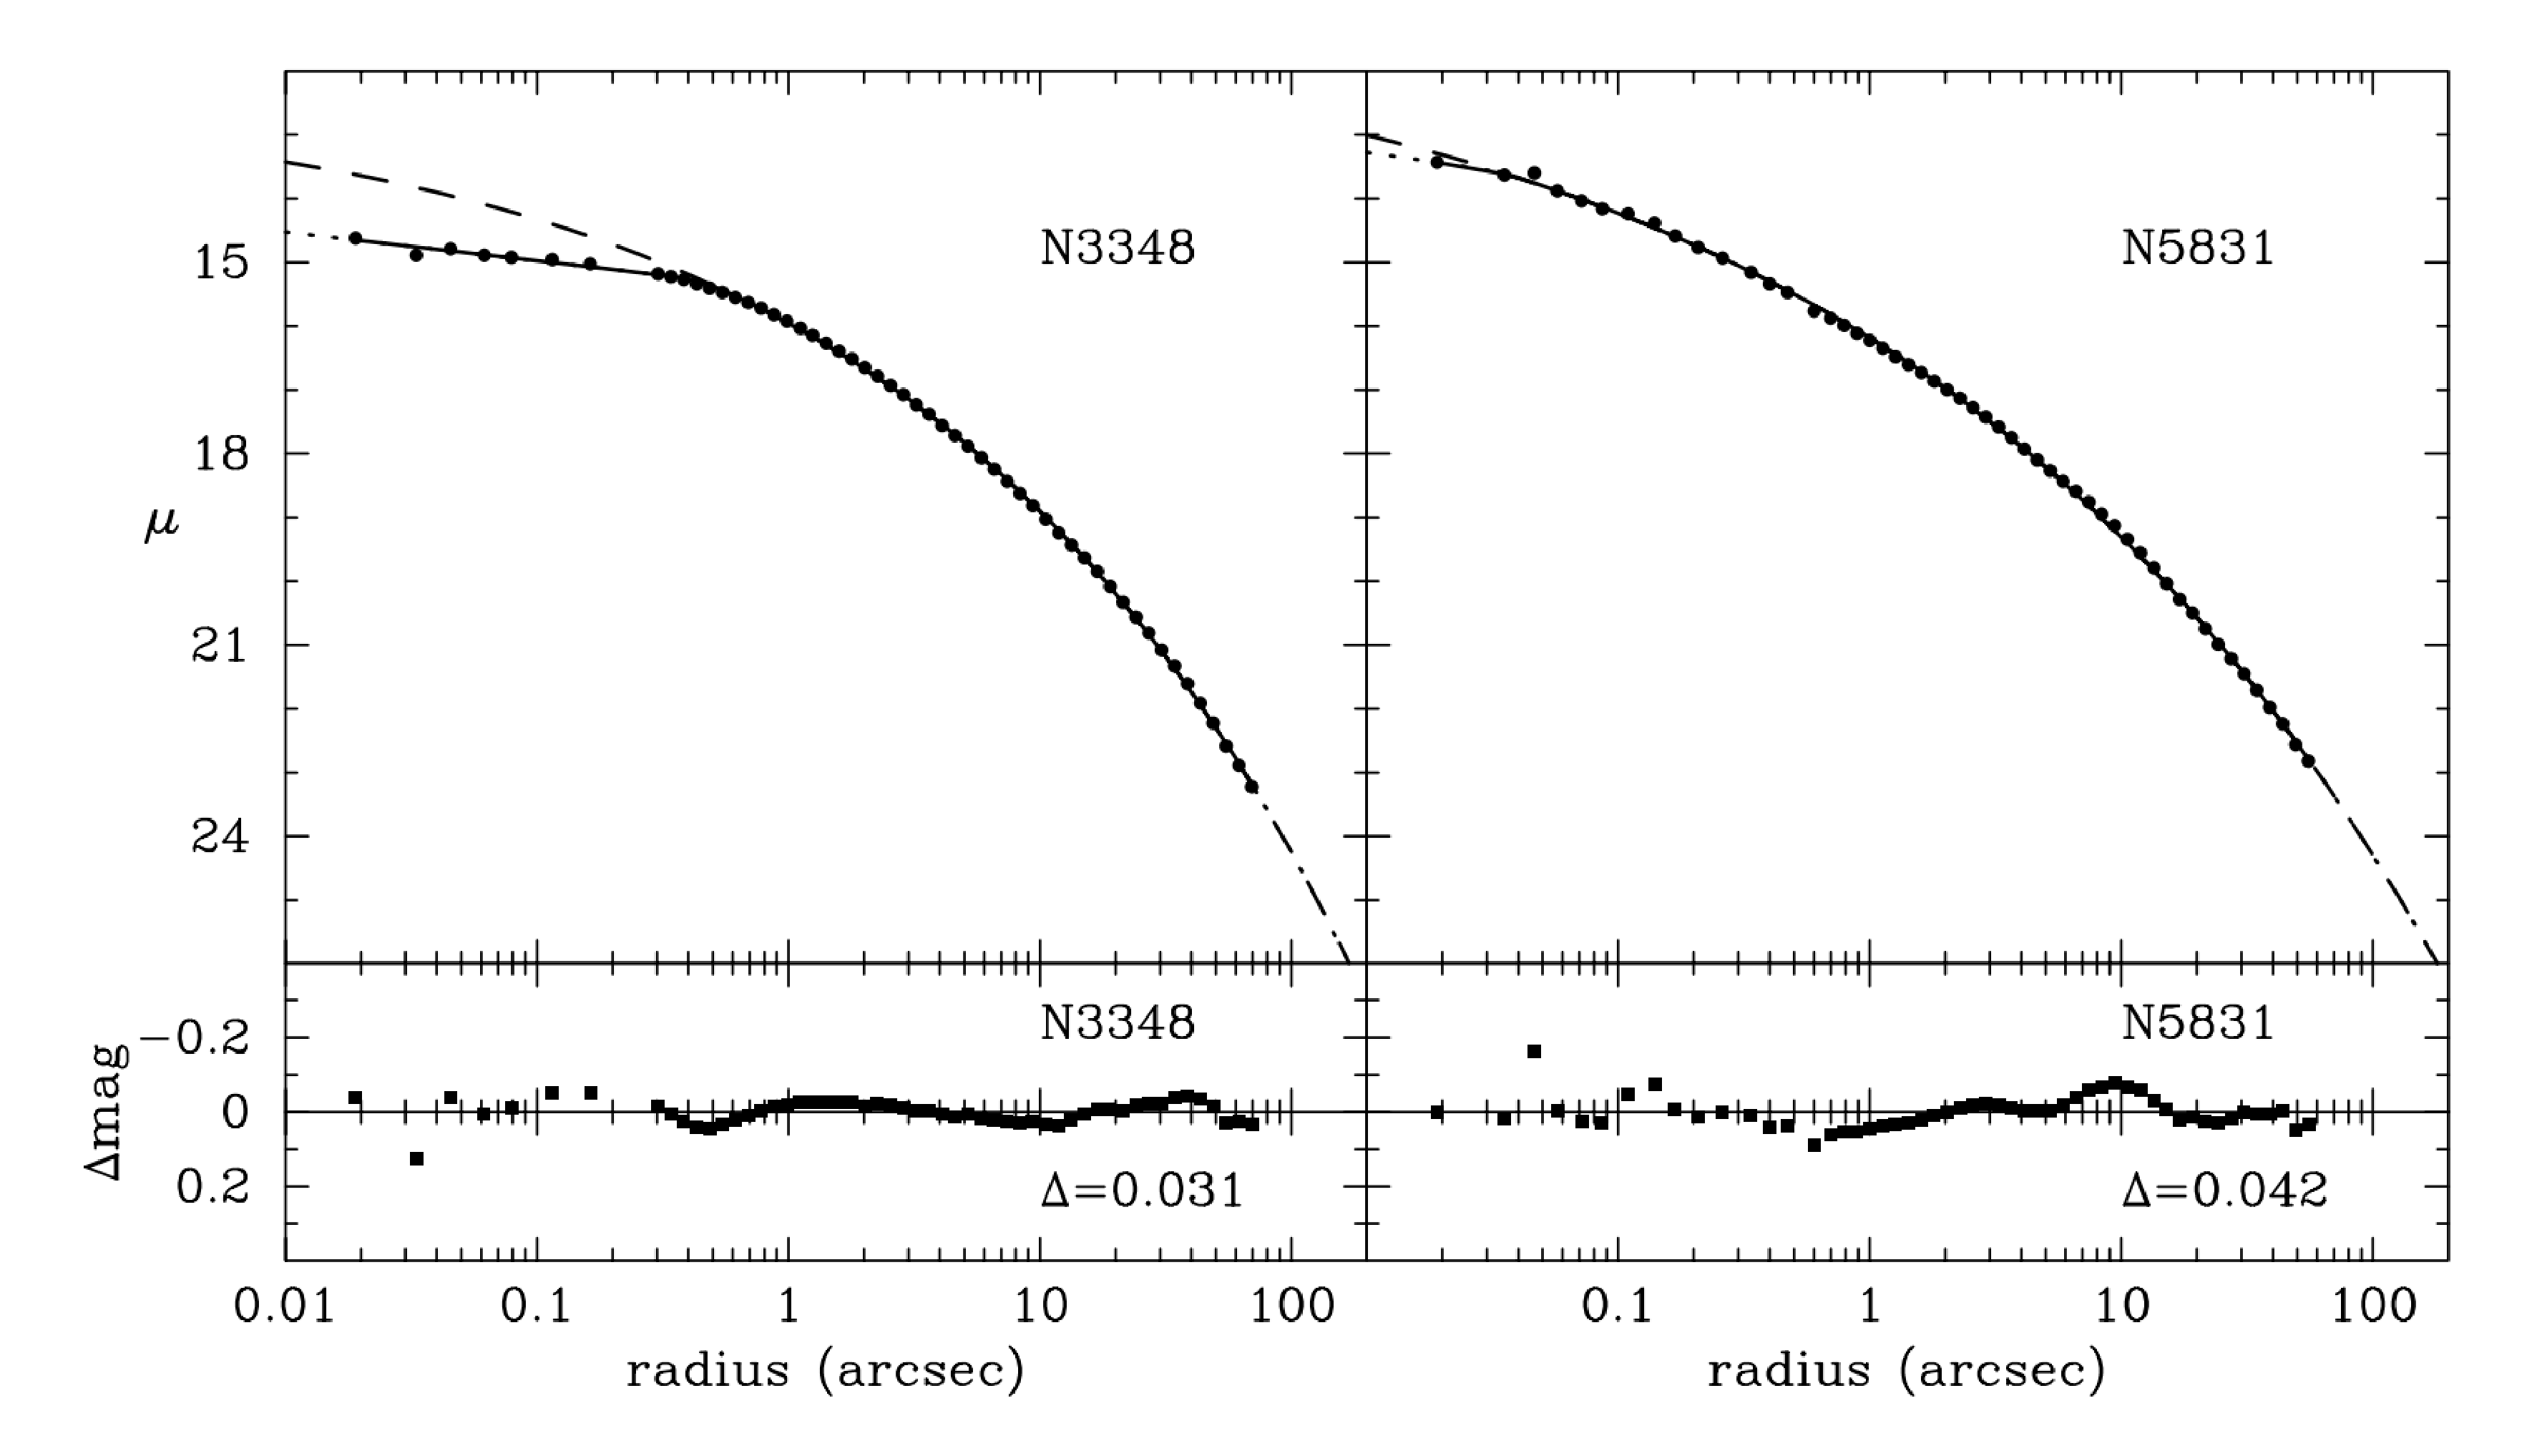
\includegraphics[width=0.9\textwidth]{images/sersiccoresersic.eps}
\end{center}
\caption{
The observed major-axis surface brightness radial profiles ($\mu$, in units of $\rm mag~arcsec^{-2}$) 
of the elliptical galaxies NGC 3348 and NGC 5831 
are shown with the black points in the top left and right panels, respectively. 
The solid lines are fits using the empirical core-S\'ersic model, 
and the dotted extensions are their inner and outer extrapolations. 
The long dashed lines indicate extrapolations of the outer S\'ersic-like part of the core-S\'ersic model. 
The residuals from the fits ($\Delta \mu = data - model$) are shown with black squares in the bottom panels, 
and the rms scatter $\Delta$ is given for each fit. 
This Figure was extracted from \cite{graham2003coresersicmodel}. }
\label{fig:corser}
\end{figure}

Partially depleted cores are believed to form during dissipationless (``dry'', i.e.~gas-poor) mergers \citep{begelman1980}, 
where the progenitor black holes sink towards the centre of the remnant galaxy due to dynamical friction against stars, 
form a bound pair and further reduce their orbital separation by transferring their binding energy to the surrounding stars 
via a three-body scattering process also known as ``gravitational slingshot'' 
(\citealt{milosavljevicmerritt2001,merritt2013CQG}, and references therein). 
The scouring action of the black hole binary has the effect of lowering the galaxy's stellar central density, 
in fact producing a partially depleted core 
(e.g.~\citealt{merritt2006RPP,dotti2012,colpi2014}). 
The lack of a significant amount of gas during the merger is a necessary condition 
to guarantee the formation of a partially depleted core. 
\cite{mayer2009} and \cite{colpi2009} followed the simulations of two merging Milky Way-like galaxies 
and reported that the time-scale for the formation of a close black hole binary system due to dynamical friction against gas 
is $\approx$100 times shorter than that due to dynamical friction against stars. 
Therefore, a black hole binary coalesces more quickly in a gas-rich (``wet'') merger than in a gas-poor (``dry'') merger, 
i.e.~when gas is in play, the binary does not have enough time to form a partially depleted core. 
In addition, gas is likely to be funnelled towards the centre of the galaxy remnant, shock and induce star formation, 
which would act against the formation of a core by increasing the central stellar density. 


\subsection{Origin of SMBHs}
As of today, the formation of SMBHs is still an unsolved puzzle. 
The key astrophysical questions that pertain to this open debate are: 
(\emph{i}) what are the initial seeds of SMBHs and when did they form? 
(\emph{ii}) how were these seeds distributed in the early universe 
(i.e.~what is their mass distribution function and space density)? 
and (\emph{iii}) what is their accretion history throughout the Universe's first few billion years? 
\cite{volonteribellovary2012} review three possible pathways -- not mutually exclusive -- 
that have been proposed as viable mechanisms to SMBH seeds formation. \\

The first of these three theoretical scenarios states that SMBHs originated from the remnants of Population III stars. 
Population III stars are the (hypothetical) first generation of stars, which formed out of zero-metallicity pristine gas. 
The lack of metals implies inefficient cooling and inefficient fragmentation of the gas, 
making possible to produce very massive stars (with initial masses $\gtrsim 100~\rm M_\odot$). 
The fate of Population III stars mainly depends on their initial mass \citep{heger2003}. 
A low-metallicity star that initially weights $\approx 25 - 140~\rm M_\odot$ is predicted to directly collapse into a black hole 
with about half of the mass of its progenitor star. 
Such black hole would not be heavy enough to be dragged by dynamical friction towards the host galaxy centre, 
therefore it would hardly contribute to the formation of a central SMBH. 
Between $\approx 140 - 260~\rm M_\odot$, low-metallicity stars lie within the pair instability supernova regime, 
where the final nuclear-powered explosion completely disrupts the star and leaves no remnant. 
Above $\approx 260~\rm M_\odot$, the nucleus of a low-metallicity star is highly unstable 
and quickly ($\approx 2~\rm Myr$) collapses into a black hole that retains at least half of the initial stellar mass. 
For many years, these high-mass stellar black holes have been considered the most promising SMBH seeds candidates. 
However, as recent numerical simulations were improved 
thanks to the achievement of better resolution and the inclusion of more complex physics 
(e.g.~\citealt{turk2009,greif2011,clark2011,stacy2012}), 
it became clear that fragmentation played a more important role in the formation of Population III stars, 
which turned into less attractive candidates for the origin of SMBHs. \\

A second possibility for the genesis of SMBH seeds is the formation of a supermassive star (up to $\approx 10^6~\rm M_\odot$) 
at the centre of a primordial galaxy. 
In this scenario, low-metallicity, low-angular momentum gas infalls towards the bottom of the potential well of a dark matter halo and, 
due to gravitational instabilities, does not settle into a rotationally supported disc, 
but accumulates into a very massive star, 
whose core rapidly ($\approx 1~\rm Myr$) collapses into a black hole and swallows the surrounding gas envelope, 
giving birth to a $\approx 10^3 - 10^6~\rm M_\odot$ SMBH seed. \\

According to the third theoretical scenario, gas infalls towards the centre of a dark matter halo and fragments into several stars
that form a dense stellar cluster. 
Before the first supernova explosions can occur, small stars collide with each other within the cluster 
and merge into a massive ($\approx 10^3~\rm M_\odot$) star which eventually collapses into a black hole with similar mass. \\

The discovery of ultraluminous quasars at $z>6$ has accentuated the urge to create very massive black hole seeds in a relatively short time 
(e.g.~\citealt{alexandernatarajan2014,madau2014,lupi2015}). 
To date, there have been nearly 50 claims of $z>6$ quasars hosting $\gtrsim 10^9~\rm M_\odot$ black holes 
(e.g.~\citealt{fan2003,jiang2007,mortlock2011,banados2014,trakhtenbrot2015,wu2015}). 
Within a $\Lambda$CDM cosmology, such early giant monsters could not have formed so quickly 
without the creation of anomalously massive seeds 
or incredibly high accretion rates, i.e.~exceeding the Eddington limit 
(but see \citealt{meliamcclintock2015} for an alternative explanation). 
However, it is worth noting that these black hole masses are calculated with the reverberation mapping method, 
assuming that $M_{\rm BH}$ is directly proportional to the virial factor $f$, 
which is calibrated on the normalisation of the $z=0$ observed $M_{\rm BH} - \sigma_*$ correlation. 
The existence of (unknown) selection biases in the local sample of directly measured black hole masses 
would imply a systematic overestimation of the virial factor and, consequently, 
of the black hole masses estimated with the reverberation mapping technique. \\


%\subsection{bhfp}
%\cite{marconihunt2003} pointed out a significant correlation between the residuals of the $M_{\rm BH} - \sigma_*$
%relation and the effective radii of the spheroids in their sample. 
%Motivated by this observation, many studies have explored the possibility that the different black hole mass 
%scaling relations were projections of the same black hole ``fundamental plane'' (BHFP), in analogy to the
%well known fundamental plane of spheroids ($R_{\rm e,sph} \propto \sigma_{*}^{\alpha} \langle \mu_{\rm e,sph}\rangle^{\beta}$,
%with $\langle \mu_{\rm e,sph}\rangle$ the mean bulge surface brightness within $R_{\rm e,sph}$, \citealt{djorgovskidavis1987}).
%Various three-parameter correlations have been investigated, in the form of $M_{\rm BH} - R_{\rm e,sph} - \langle \mu_{\rm e,sph}\rangle$ 
%\citep{barwaykembhavi2007}, 
%$M_{\rm BH} - R_{\rm e,sph} - \sigma_{*}$ \citep{marconihunt2003,defrancesco2006,allerrichstone2007,
%hopkins2007} and $M_{\rm BH} - R_{\rm e,sph} - n_{\rm sph}$ \citep{graham2008}.
%However, \cite{graham2008} revisited all the three versions of the BHFP and showed that none of them is defined by the population
%of barless spheroids. 
%In fact, the bulges of barred spiral galaxies systematically deviate from the $M_{\rm BH} - \sigma_*$ relation, 
%producing the apparent black hole plane. 
%\cite{graham2008} nevertheless pointed out that more and better quality data would be welcome in fully resolving this issue.
%
%
%This observation motivated \cite{hopkins2007} to search for a black hole ``fundamental plane'' (BHFP), in analogy to the
%well known fundamental plane of spheroids ($R_{\rm e} \propto \sigma_{*}^{\alpha} I_{\rm e}^{\beta}$).
%They found that the systems in their sample lie on a BHFP of the form $M_{\rm BH} \propto \sigma_{*}^{3.0} R_{\rm e}^{0.5}$ 
%or $M_{\rm BH} \propto M_{*}^{0.5 - 0.7} \sigma_{*}^{1.5 - 2.0 }$.


%\subsection{fundamental corr}

\subsection{Monster black holes}
\label{sec:monsters}
Over the last five years, several claims of detections of \emph{over-massive} black holes accumulated in the literature. 
Over-massive black holes are black holes whose mass is significantly larger 
than what is expected from the galaxy's spheroid stellar velocity dispersion or stellar mass, 
i.e.~they are positive outliers in the $M_{\rm BH} - \sigma_*$ or $M_{\rm BH} - M_{\rm *,sph}$ diagrams. \\

Using integral-field spectrographs at the Gemini North and Keck 2 telescopes, 
\cite{mcconnell2011} targeted the BCGs (NGC 3842 and NGC 4889) of two massive galaxy clusters, 
the Leo and Coma clusters (Abell 1367 and Abell 1656, respectively), 
and reported the direct detection of the two most massive black holes ever found at that time. 
They claimed that these two black holes are significantly more massive 
than predicted by the popular $M_{\rm BH} - \sigma_*$ and $M_{\rm BH} - L_{\rm sph}$ correlations, 
and speculated that the growth of the largest galaxies and their black holes happens by means of evolutionary processes 
different from what is commonly assumed for less massive elliptical galaxies. \\

\cite{rusli2011} obtained SINFONI integral-field unit observations of the nuclear region of the galaxy NGC 1332 
and measured a one billion solar masses black hole, 
consistent with the galaxy's stellar velocity dispersion, 
but offset from the $M_{\rm BH} - L_{\rm sph}$ relation by a full order of magnitude. \\

\cite{vandenbosch2012} combined archival Hubble Space Telescope (\emph{HST}) high-resolution imaging 
and long-slit spectroscopy (obtained with the Marcario Low Resolution Spectrograph on the Hobby-Eberly Telescope, Texas) 
of the nuclear region of the galaxy NGC 1277, 
and directly measured the central black hole mass by fitting self-consistent Schwarzschild models 
to the integrated stellar kinematics. 
They found a twenty billion solar masses black hole, 
which they estimated to weight 59\% of the host spheroid's mass (or 14\% of the galaxy's total stellar mass). 
According to their measurement, 
the black hole of NGC 1277 was an order of magnitude more massive than what expected from the host spheroid's stellar velocity dispersion 
and two orders of magnitude more massive than what expected from the host spheroid's stellar mass.
\cite{emsellem2013} re-analysed \citeauthor{vandenbosch2012}'s data 
and showed that their observations were consistent with a black hole mass up to an order of magnitude smaller 
than the extraordinary value previously reported. 
However, \cite{yildirim2015} and \cite{scharwachter2015} confirmed \citeauthor{vandenbosch2012}'s measurement. \\

\cite{bogdan2012} reported on the unusually high $M_{\rm BH}/M_{*,sph}$ ratio for the galaxies NGC 4342 and NGC 4291 
and concluded that no co-evolution subsisted between these two galaxies and their black holes. 
Other reportedly over-massive black holes belong to the galaxies NGC 1271 \citep{walsh2015} and Mrk 1216 \citep{yildirim2015}. \\

On the basis of these claims, \cite{ferremateu2015} theorised that, 
while most today's massive early-type galaxies have completed their two-phase growth path (``in-situ'' and ``ex-situ''), 
the over-massive black holes hosts skipped the second (``ex-situ'') phase and therefore represent an exception. 


\section{Galaxy decomposition}
Galaxy decomposition is a parametric analysis that allows one to fit the surface brightness distribution
of galaxies using a combination of analytic functions (usually one function per
galaxy component, such as spheroid, disc, bar, nucleus, etc.). 
The 1D (one-dimensional) technique begins with fitting isophotes to the galaxy image.
Isophotes are curves along which the intensity of light is constant 
and they are typically described with concentric ellipses.  
The 1D surface brightness radial profile is then extracted and modelled with a combination of 1D analytic functions. 
With the 2D (two-dimensional) technique one fits 2D analytic functions directly to digital images. 
Galaxy decomposition is useful to perform structural analysis of galaxies and obtain the best-fit 
parameters of the spheroidal component, such as the luminosity, the half-light radius 
and the central radial concentration of stars. \\

\begin{figure}[htb]
\begin{center}
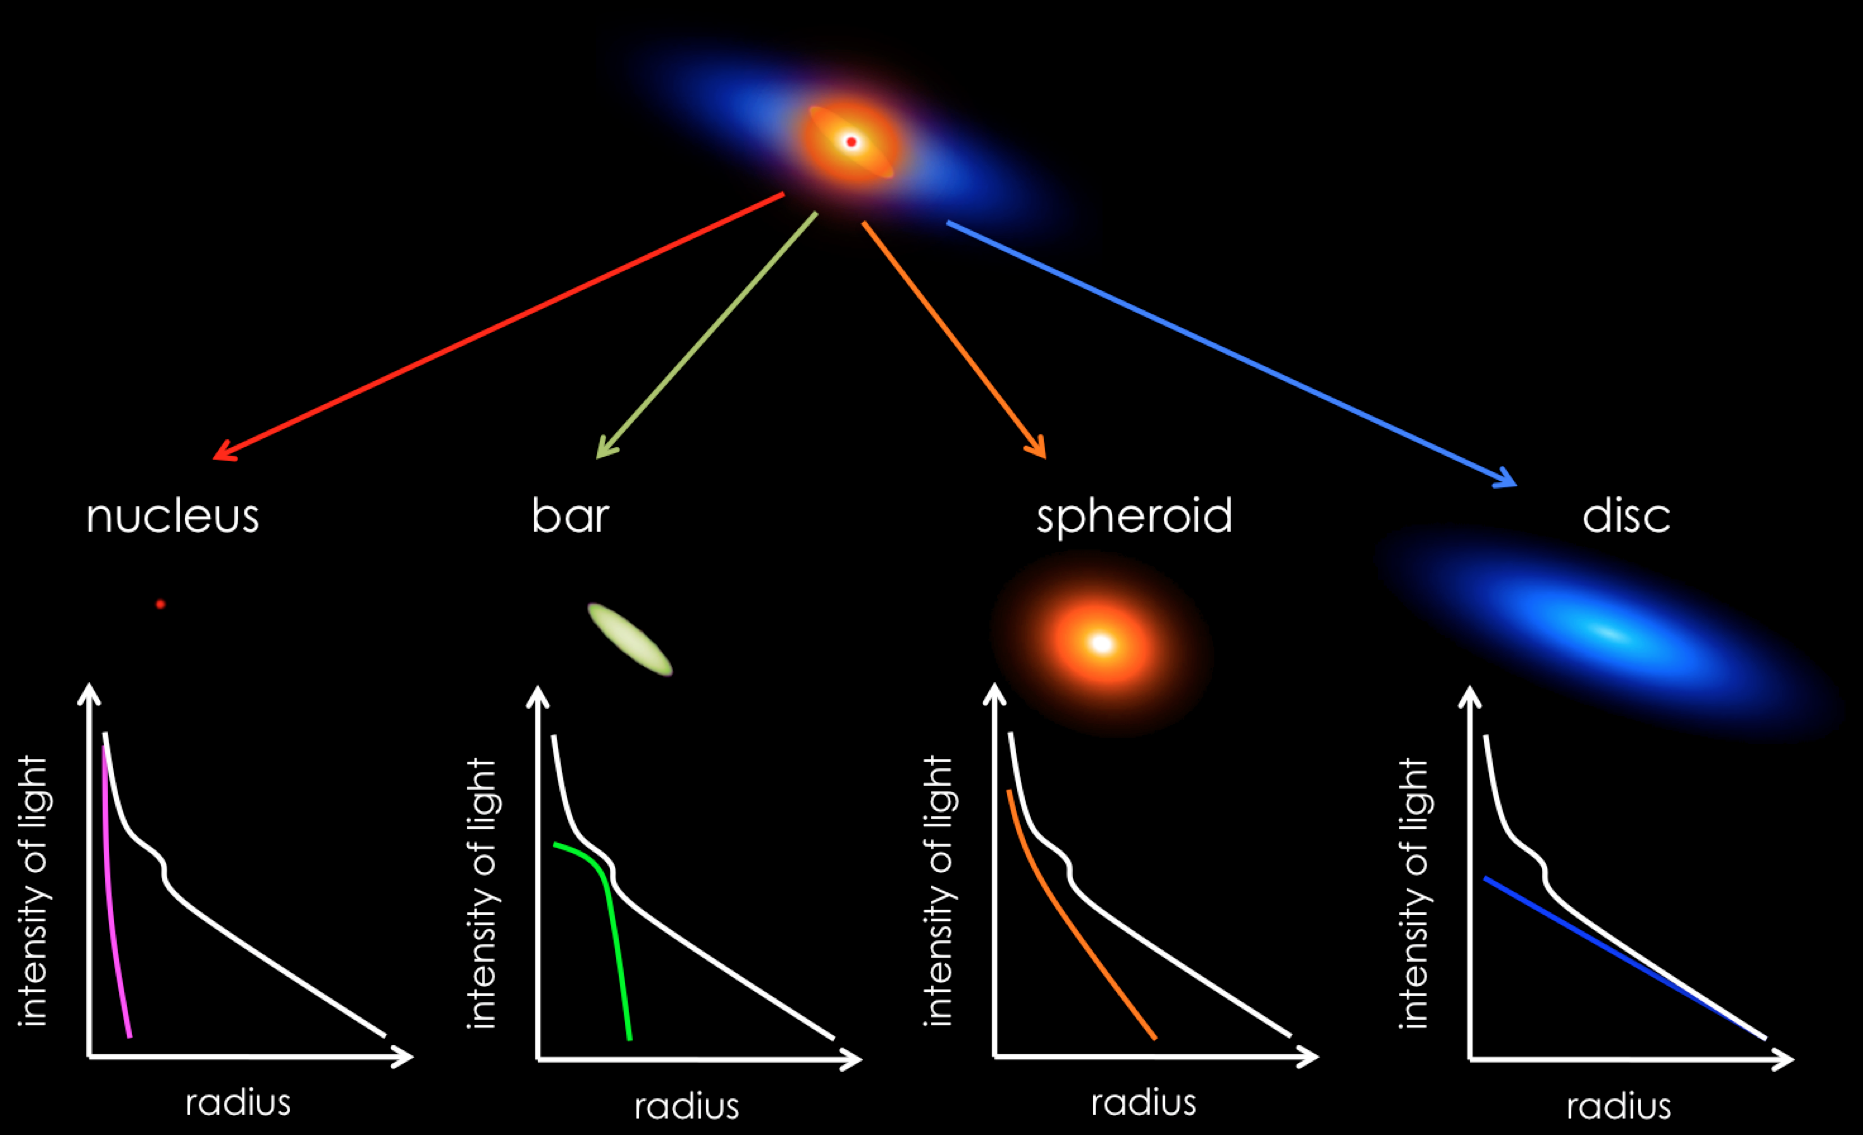
\includegraphics[width=\textwidth]{images/galaxyvivisection.eps}
\end{center}
\caption{Schematic representation of one-dimensional galaxy decomposition. 
The mock galaxy at the top is composed of a spheroid (orange), a large-scale disc (blue), 
a bar (green), and a nuclear source (red). 
The observed surface brightness profile of the galaxy (intensity of light as a function of galactocentric radius) 
is the white curve. 
The contribution of each galaxy component to the total surface brightness profile is modelled with one analytic function, 
illustrated with a solid line of the same colour as the corresponding component. 
The sum of all analytic functions gives the total galaxy model, 
which is matched to the observed surface brightness profile. }
\end{figure}

Pioneer studies that performed 1D bulge/disc decompositions of galaxies (e.g.~\citealt{simiendevaucouleurs1986}) 
described the bulge component with a \cite{devaucouleurs1948} $R^{1/4}$ profile:
\begin{equation}
\mu_{\rm de Vaucouleurs}(\mu_{\rm e},R_{\rm e};R) = \mu_{\rm e} + 8.32678
\Biggl[\biggl(\frac{R}{R_{\rm e}}\biggr)^{1/4}-1\Biggr] ,
\end{equation} 
and the disc component with an exponential profile:
\begin{equation}
\mu_{\rm exponential}(\mu_{\rm 0},h;R) = \mu_{\rm 0} + \frac{2.5}{\ln(10)} \biggl(\frac{R}{h} \biggr) .
\end{equation} 
Here $\mu$ is the surface brightness profile, 
$R$ is the projected galactic radius, i.e.~the distance of the isophotes from the galaxy centre, 
$R_{\rm e}$ is the bulge effective radius (or half-light radius) that encloses half of the total light from the model, 
$\mu_{\rm e}$ is the bulge surface brightness at the effective radius, 
$\mu_{\rm 0}$ is the disc central surface brightness, 
and $h$ is the disc scale length. \\

However, it soon became clear to some that the fixed curvature of the two-parameter de Vaucouleurs $R^{1/4}$ law 
was not adequate to accommodate the variety of shapes observed in the light profiles of stellar spheroidal systems. 
A more ductile mathematical function was needed 
such as the three-parameter \cite{sersic1963,sersic1968} $R^{1/n}$ model: 
\begin{equation}
\mu_{\rm S\acute{e}rsic}(\mu_{\rm e},R_{\rm e},n;R) = \mu_{\rm e} + \frac{2.5~b_{\rm n}}{\ln(10)} 
\Biggl[\biggl(\frac{R}{R_{\rm e}}\biggr)^{1/n}-1\Biggr] ,
\end{equation}
where the S\'ersic index $n$ is the parameter that measures the curvature of the radial light profile,
and $b_{\rm n}$ is a scalar value defined in terms of the S\'ersic index 
(see \citealt{grahamdriver2005} for a valuable compendium). 
After \cite{caon1993} and \cite{donofrio1994} demonstrated the superiority of the S\'ersic model 
over the de Vaucouleurs law in describing the spatial distribution of light of early-type galaxies, 
the varying curvature of the S\'ersic model became a necessity also for rendering 
the light profiles of the bulges of spiral galaxies 
\citep{andredakis1995,moriondo1998,grahamprieto1999,khosroshahi2000,graham2001}. \\

Thanks to the improved computational speed of machines, 
2D fitting algorithms have become more and more popular over the last two decades. 
\cite{dejong1996} presented a 2D decomposition technique 
which allowed one to model the surface photometry of a galaxy 
using an exponential light profile for both the bulge and the disc. 
\cite{simard1998} developed the IRAF\footnote{IRAF is the Image Reduction and Analysis Facility, 
distributed by the National Optical Astronomy Observatory, 
which is operated by the Association of Universities for Research in Astronomy (AURA) 
under cooperative agreement with the National Science Foundation.} package {\tt GIM2D}, 
a 2D decomposition code aimed at distant galaxies. 
{\tt GIM2D} takes an input image and simultaneously decomposes all the objects 
as the sum of a S\'ersic and an exponential profile. \\

A major breakthrough came with {\tt GALFIT}, 
a 2D fitting algorithm released by \citeauthor{peng2002} (\citeyear{peng2002}; 
the nowadays popular {\tt GALFIT3}, an improved version of the original algorithm, was presented by \citealt{peng2010}), 
which marked an important turning point for the quantitative morphological analysis of galaxies. 
Thanks to its capability of fitting a galaxy with an arbitrary number of components 
-- chosen from a wide variety of analytical functions such as the S\'ersic and the ``Nuker'' models, 
or the exponential, Gaussian, and Moffat profiles -- 
and to its optimisation in computational speed, 
{\tt GALFIT} was specifically conceived for modelling large images of spatially well-resolved, 
nearby galaxies observed with the Hubble Space Telescope. \\

\cite{desouza2004} developed {\tt BUDDA} (Bulge/disc Decomposition Analysis), 
a code to perform 2D decomposition of galaxies using a two-component S\'ersic+exponential model. 
The number of fitted components was intentionally limited to two (bulge+disc), 
with the purpose of using the residual images 
to study the additional substructures such as bars, lenses, rings, and inner discs. \\

\cite{laurikainen2005} opted for a hybrid approach, 
combining the advantages of a 2D decomposition technique 
with the insight gained from a 1D isophotal analysis. 
In this exemplary study, the authors modelled the images of 24 early-type disc galaxies (S0/S0a) 
accounting for bulge, disc, bars, ovals/lenses\footnote{According to their nomenclature, 
an egg-shaped structure (with axis ratio $b/a \gtrsim 0.85$) 
embedded within the large-scale disc of a galaxy 
is dubbed lens or oval in case of a lenticular or spiral galaxy, respectively. 
Lenses/ovals and pseudobulges might have similar ellipticities, 
but the former typically have lower surface brightness and sharper outer edges than the latter 
\citep{kormendykennicutt2004}. }, and inner discs. 
Their decomposition method was assessed on synthetic images of galaxies composed of a bulge, 
a large-scale disc, and a bar. 
They tested the effects of the omission of the bar component from the galaxy model. 
While a three-component (bulge+disc+bar) model was correctly recovering the real bulge parameters, 
a two-component (bulge+disc) model was overestimating the bulge luminosity by up to 40\% 
because the S\'ersic model for the bulge was somehow ``forced'' to account also for the bar. 
They also experimented with a large number of different weighting maps, 
and concluded that the results from the fit were not significantly dependent on the choice of the weighting function,
unless the signal-to-noise of the galaxy image was extremely low, 
or a prominent component was not included in the model. 
In addition, they pointed out that a fit lacking seeing correction resulted in notably biased bulge parameters. 
\cite{laurikainen2005} stressed an important point about galaxy decomposition: 
in order to have control of the physical meaning of the different components in a galaxy, 
\emph{a priori} evaluation of the existence of such components is required. 
This concept is opposed to the (nowadays popular) approach of repeating the fit of a galaxy 
by continuously increasing the number of model components 
until all residual structures are eliminated from the residual image.  
\cite{laurikainen2005} used three different methods to identify the structural components of a galaxy:
they inspected (\emph{i}) the radial profiles of ellipticity and position angle of the galaxy's isophotes, 
whose bumps often correspond to bars, ovals/lenses, and inner discs 
when these components are sufficiently bright compared to the large-scale disc, 
(\emph{ii}) the radial profiles of low azimuthal wavenumber Fourier amplitudes and phases, 
sensitive to weak bars and ovals/lenses, 
and (\emph{iii}) the unsharp masks\footnote{Unsharp masks are obtained from the original images 
with a mathematical operation of convolution. By suppressing large-scale, low-frequency variations 
in the images, they act as a filter and reveal faint asymmetric structures within the galaxies 
\citep{malinzealey1979,erwinsparke2003}.}, useful to reveal the innermost structures. 
Upon comparing the results from their three-component decompositions 
with those obtained from the two-component decompositions of \cite{simiendevaucouleurs1986} in the B-band 
and \cite{desouza2004} in the K$_S$-band, 
\cite{laurikainen2005} noted that their bulge-to-total ratios were considerably smaller for all Hubble types. 
This large discrepancy was not due to the wavelength used, 
but to the fact that, when a galaxy model does not account for a bar, 
a large fraction of the bar light erroneously goes into the bulge model, 
artificially increasing the bulge-to-total ratio. 
This sophisticated decomposition method was applied to the analysis of 175 early-type disc galaxies 
using deep near-infrared imaging \citep{laurikainen2007,laurikainen2010},  
and the results from these decompositions were used for a detailed study of bars, ovals/lenses and bulges. 
They found ovals/lenses in 70\% of the S0/S0a galaxy sample, 
and nuclear components (bars/rings/discs) in 50\% of them. 



\subsection{Photometry and kinematics}
\label{sec:photokin}
Early-type galaxies can exhibit a wide variety of kinematic features, 
going from the fainter rotationally-supported systems to the brighter dispersion-dominated ones (e.g.~\citealt{davies1983}). 
While the identification of stellar discs in images of spiral galaxies is generally trivial thanks to the presence of spiral arms, 
featureless discs in bright, early-type galaxies can be particularly hard to recognise 
by looking at the photometry alone, due to well-known inclination effects (e.g.\citealt{rixwhite1990,gerhardbinney1996}). 
However, this problem can be alleviated with the use of kinematic information
(e.g.~\citealt{carter1987,franx1989,nieto1991,rixwhite1992,cinzanovandermarel1993,donofrio1995,graham1998fornax}).
In particular, our understanding of the internal structure of early-type galaxies has undoubtedly improved over the past decade 
thanks to the introduction of integral-field spectrographs and the analysis of two-dimensional kinematic maps 
(e.g.~the ATLAS$^{\rm 3D}$ survey, \citealt{cappellari2011}). \\

\cite{emsellem2007} used the specific angular momentum within one effective radius 
($\lambda_{\rm R} = \langle R |V| \rangle / \langle R \sqrt{V^2 + \sigma^2} \rangle $, 
where $R$ is the semimajor-axis radius, $V$ is the mean velocity and $\sigma$ is the velocity dispersion)  
and the ellipticity at one effective radius 
($\epsilon = 1 - (b/a)$, 
where $(b/a)$ is the ratio of minor-to-major axis length) 
to classify early-type galaxies into fast rotators and slow rotators, 
based on the empirical divide $\lambda_{\rm R} = 0.31 \sqrt{\epsilon}$. \\

\cite{krajnovic2006} developed ``kinemetry'', 
a method that combines surface photometry and kinematics 
to recognise less obvious structures in galaxies, such as embedded discs and kinematic subcomponents. 
Using kinemetry, \cite{krajnovic2011} measured the regularity of velocity maps 
and demonstrated that fast rotators are typically nearly axisymmetric systems, 
whereas most slow rotators are triaxial systems. 
At present, the joint effort of imaging and integral-field spectroscopy is undeniably our best chance 
to disclose the internal structure of galaxies (e.g.~\citealt{krajnovic2015IAUS}).  \\

Putting this paradigm into practice, 
\cite{krajnovic2013} compared photometric signatures and kinematic properties of stellar discs 
for the 180 unbarred early-type galaxies of the ATLAS$^{\rm 3D}$ sample. 
For each galaxy, they fit the light distribution using a single bulge \citep{sersic1963,sersic1968} 
and a bulge+disc (S\'ersic+exponential) model, 
preferring the latter when the improvement over the single bulge model was substantial 
and no correlation within the residuals was observed. 
They found that exponential sub-components in fast rotators correspond 
to a genuine family of rotationally-supported discs or disc-like structures, 
which were identified in 83\% of the unbarred early-type subsample,
contributing to 40\% of the total stellar mass and  
covering a full range of disc-to-total flux ratios. 
From their analysis, \cite{krajnovic2013} concluded that, when using photometry only, 
inclination effects do not particularly affect the identification of dominant discs, 
but they become much more disruptive when dealing with low-inclination, medium size discs. 
The use of kinematics is therefore the best approach to mitigate inclination effects. 
One of the key results obtained by the ATLAS$^{\rm 3D}$ Collaboration is that 
the majority of early-type galaxies contain stellar discs 
with an essentially continuous distribution of disc-to-total flux ratios, 
which led \cite{cappellari2011} to the introduction of a new classification scheme 
aimed at replacing the classical Hubble diagram. \\



\subsection{A compendium of the previous literature }
Over the past nine years, five independent studies 
\citep{grahamdriver2007,sani2011,vika2012,beifiori2012,lasker2014data,lasker2014anal}
have attempted galaxy decomposition 
for samples of galaxies with a direct measure of the black hole mass. 
The main aim of each study was to derive the parameters of the spheroidal components of their galaxies 
and explore correlation with the black hole mass.
Table \ref{tab:lit} summarises the main characteristics and findings of each work. 
%The last column refers to the study presented in this thesis 
%and highlights its improvements over the past literature.

\begin{table}[ht] 
\footnotesize
%\small
\centering 
\begin{tabular}{llllll}
\hline\hline 
		       & {\bf GD07}	 & {\bf S+11}	   & {\bf V+12} & {\bf B+12}  & {\bf L+14} \\ 	      %& {\bf This work}   \\ 
\hline \\ [-1.5ex]
{\bf Galaxies }        & 27		 & 57		   & 25 	& 19	      & 35	   \\	      %& 66		  \\
{\bf Wavelength }      & R-band 	 & $3.6~\mu \rm m$ & K-band	& $i$-band    & K-band     \\	      %& $3.6~\mu \rm m$   \\
{\bf Decomposition}    & 1D		 & 2D		   & 2D 	& 2D	      & 2D	   \\	      %& 1D \& 2D	  \\
{\bf Nuclei }	       & masked 	 & modelled	   & modelled	& not treated & modelled    \\	      %& modelled/masked    \\
{\bf Cores }	       & masked 	 & masked	   & masked	& not treated & masked     \\ 	      %& masked  	  \\ 
{\bf Bars }	       & excluded	 & modelled	   & modelled	& excluded    & modelled    \\ 	      %& modelled 	  \\ 
{\bf Other components} & no		 & no		   & no 	& no	      & yes	   \\ 	      %& yes		  \\ 
{\bf Kinematics}       & no		 & no		   & no 	& no	      & no	   \\ [0.5ex] %& yes		  \\ [0.5ex] 
\hline
\multicolumn{6}{c}{\emph{Conclusions}} \\ 
\hline \\ [-1.5ex]
$\boldsymbol{ M_{\rm BH}-n_{\rm sph}}$  		& yes	& no	     & no  & no        & -	     \\ 	%& -   \\
$\boldsymbol{ M_{\rm BH}-L_{\rm sph}}$  		& -	& yes	     & yes & yes       & fundamental \\ 	%& -   \\
$\boldsymbol{ M_{\rm BH}-M_{\rm sph,dyn}}$		& -	& yes	     & -   & yes       & -	     \\ 	%& -   \\
$\boldsymbol{ M_{\rm BH}-M_{\rm sph,*}}$		& -	& yes	     & -   & -         & -	     \\ 	%& -   \\
$\boldsymbol{ M_{\rm BH}-R_{\rm e}}$			& -	& secondary  & -   & -         & -	     \\ 	%& -   \\
$\boldsymbol{ M_{\rm BH}-\langle \mu_{\rm e} \rangle}$  & -	& -	     & -   & no        & -	     \\ 	%& -   \\
$\boldsymbol{ M_{\rm BH}-L_{\rm gal}}$  		& -	& -	     & -   & secondary & fundamental \\ [0.5ex] %& -   \\ [0.5ex] 
\hline 
\hline 
\end{tabular}
\caption{ Main characteristics and findings of the latest five studies that have attempted galaxy decomposition 
to derive and explore black hole mass scaling relations. 
The number of galaxies accounts only for those with a direct measurement of the black hole mass 
(no upper limits are considered here). 
GD07 = \cite{grahamdriver2007}; S+11 = \cite{sani2011}; V+12 = \cite{vika2012}; B+12 = \cite{beifiori2012}; 
L+14 = \cite{lasker2014data,lasker2014anal}.}
\label{tab:lit} 
\end{table}

\cite{sani2011} used galaxy images 
obtained with the \emph{Spitzer} satellite in the $3.6~\mu \rm m$ wavelength-band, 
which currently represents the best proxy for the stellar mass, 
even superior to the K-band (\citealt{sheth2010}, and references therein). \\

%Besides using the largest sample of galaxies to date, 
%this work is based on observations in the $3.6~\mu \rm m$ wavelength-band, obtained with the \emph{Spitzer} satellite,
%which currently represents the best proxy for the stellar mass (\citealt{sheth2010}, and references therein). 
There has been an ongoing debate as to whether 2D galaxy decomposition techniques should be preferred over 1D techniques. 
The performance of each method can vary according to different technical factors 
(such as the signal-to-noise of the galaxy images, the accuracy of the description of the Point Spread Function, 
the gradient of ellipticity and position angle of the galaxy isophotes, 
the fitting weighting scheme, etc.), 
therefore advantages and disadvantages are not absolute and depend on the individual science case. 
To our best knowledge, 
no published study has ever been conducted on a systematic comparison between 1D and 2D galaxy decomposition techniques. \\

%we chose to experiment with both methods and compare the results. 
Previous works have demonstrated that, when studying galaxies with a complex morphology, 
the accuracy of the recovery of the bulge parameters increases 
when all galaxy components are taken into account by the model  
\citep{laurikainen2005,gadotti2008,salo2015}. 
\cite{lasker2014data} identified and modelled more galaxy components than any other study,
but no work did it with the assistance of kinematical information. \\

Interestingly, the past studies all used almost the same sample of galaxies 
(the number of directly measured black hole masses increased with time), 
but they claimed some contradictory conclusions. 
One study obtained a good $M_{\rm BH}-n_{\rm sph}$ correlation, whereas three did not.
\cite{lasker2014anal} elected the $M_{\rm BH}-L_{\rm gal}$ relation as the fundamental one
(likewise the $M_{\rm BH}-L_{\rm sph}$), 
as opposed to \cite{beifiori2012}, who presented it as a secondary correlation.
The past studies did not converge to the same conclusions 
because their best-fit models for the same galaxy were often 
significantly different and not consistent with each other in terms 
of fitted components. 
Moreover, none of these studies attempted an individual galaxy-by-galaxy 
comparison of their models with the previous literature. 
%We have now made this comparison, identified the optimal decomposition, 
%and obtained improved black hole mass scaling relations using a large sample of galaxies.
%Our work will also present a comparison between 1D and 2D galaxy decompositions.

\section{Thesis outline}
The aim of this thesis is to refine and re-investigate several black hole mass scaling relations 
through the careful modelling of the spatial light distribution 
of a selected sample of 66 nearby galaxies. 
After obtaining robust structural parameters for the galaxies under study, 
I will explore substructure in the correlations between these parameters and the black hole mass, 
and explain discrepancies in the results presented in the past literature. \\

In Chapter \ref{ch:recov-mn} \citep{savorgnan2013}, 
we tackle the issue of the $M_{\rm BH} - n_{\rm sph}$ correlation using literature data. 
Four studies independently carried out photometric decompositions for similar samples of galaxies, 
but only one of them obtained a statistically significant $M_{\rm BH} - n_{\rm sph}$ relation. 
For each galaxy analysed by two or more studies, 
we compared the models used to fit the galaxy's spatial distribution of light, 
and found that the same galaxy was often described with remarkably different models 
in terms of number and type of sub-components. 
This was obviously resulting in significantly different best-fit parameters. 
We then collected the S\'ersic index measurements obtained by the four studies for 54 common galaxies 
with a direct measure of their black hole mass, 
rejected the most discrepant values, 
and used the remaining measurements to populate the $M_{\rm BH} - n_{\rm sph}$ diagram. 
Besides recovering a statistically significant $M_{\rm BH} - n_{\rm sph}$ relation for all galaxies, 
we also explored substructure for different galaxy morphological types 
(elliptical galaxies versus bulges of disc galaxies)
and nature of the nuclear light profile (S\'ersic versus core-S\'ersic). \\

In Chapter \ref{ch:galviv} \citep{paperI}, 
we present the 1D decompositions carried out by us for 66 local galaxies 
with a direct measure of their black hole mass. 
We describe the careful data reduction process through which 
we created the image-mosaics for these galaxies, 
using archival observations at $3.6~\mu \rm m$ obtained with \emph{Spitzer}. 
We detail our 1D galaxy decomposition technique and our method to estimate the uncertainties 
associated with the spheroid's best-fit parameters. 
Upon comparing the results obtained from our 1D and 2D galaxy models, 
we comment on the advantages and disadvantages connected with 1D and 2D decomposition techniques. 
The individual 1D galaxy decompositions are illustrated, 
along with a thorough analysis of each galaxy's structure 
and a scrupulous comparison with several past decompositions. \\
 
In Chapter \ref{ch:mm} \citep{paperII}, 
we use the results from our 1D galaxy decompositions 
to explore substructure in the $M_{\rm BH} - L_{\rm gal}$ and $M_{\rm BH} - L_{\rm sph}$ 
(or $M_{\rm BH} - M_{\rm *,sph}$) diagrams 
for different galaxy morphological types and nature of the nuclear light profile. 
Upon performing a detailed linear regression analysis using three different routines, 
we concluded that early-type (elliptical+lenticular) and late-type (spiral) galaxies 
follow two separate correlations in the $M_{\rm BH} - L_{\rm sph}$ (or $M_{\rm BH} - M_{\rm *,sph}$) diagram. 
In addition, we compared the level of intrinsic scatter 
in the $M_{\rm BH} - L_{\rm gal}$ and $M_{\rm BH} - L_{\rm sph}$ diagrams 
to address the question of whether or not the $M_{\rm BH} - L_{\rm sph}$ correlation 
is more fundamental than the $M_{\rm BH} - L_{\rm gal}$ correlation. \\

In Chapter \ref{ch:mn} \citep{paperIII}, 
we use the results from our 1D galaxy decompositions to populate 
the $L_{\rm sph} - n_{\rm sph}$ and $M_{\rm BH} - n_{\rm sph}$ diagrams. 
The analysis that we performed here is essentially analogous to that presented in Chapter \ref{ch:mm}.  
We did not observe any significant substructure in the $M_{\rm BH} - n_{\rm sph}$ diagram, 
where all galaxies, irrespective of their morphological type, define a single tight correlation. 
Consistency between the $M_{\rm BH} - n_{\rm sph}$ and other galaxy scaling relations 
is dicussed here.  \\

In Chapter \ref{ch:msigma} \citep{savorgnangraham2015}, 
we concentrate on the $M_{\rm BH} - \sigma_*$ scaling relation 
and the presence of some outlying, ``overmassive'' black holes at the high-mass end of this correlation. 
\cite{volontericiotti2013} proposed a theoretical interpretation 
to explain why central cluster galaxies tend to appear as positive outliers 
in the $M_{\rm BH} - \sigma_*$ diagram, lying above the observed $z=0$ correlation. 
According to the results from their semi-analytical models, 
central cluster galaxies experienced more dry mergers 
than the ``average'' population of massive early-type galaxies. 
Dry mergers are expected to increase the black hole mass, 
while leaving almost unchanged the stellar velocity dispersion. 
We tested the interpretation offered by \cite{volontericiotti2013} 
using the latest observational data. 
First, we updated the $M_{\rm BH} - \sigma_*$ diagram with a total of 89 galaxies 
and performed a linear regression analysis of it. 
Then, for each galaxy with a parially depleted core 
we measured the extent of dry mergers experienced by the galaxy 
by means of the ratio between the central stellar mass deficit and the black hole mass. 
We showed that no positive trend is observed between the number of dry mergers 
and the positive vertical offset from the $M_{\rm BH} - \sigma_*$ correlation. 
A similar test using the kinematics of galaxies gave consistent results, 
disproving the scenario advocated by \cite{volontericiotti2013}. \\

In Chapter \ref{ch:ellic} \citep{ellicular}, 
we tackle the issue of the ``overmassive'' black holes 
in the $M_{\rm BH} - M_{\rm *,sph}$ diagram. 
Due to inaccurate decompositions that failed to take into account the correct size of the main disc component, 
a number of galaxies (Mrk 1216, NGC 1271, NGC 1277, and NGC 1332) had their spheroid luminosity underestimated, 
which made them appear as positive outliers above the $M_{\rm BH} - M_{\rm *,sph}$ correlation. 
With the aid of photometric and kinematic information, 
we identified the radial extent of the main disc component, 
and built a galaxy model accordingly. 
We showed that when these galaxies are correctly modelled, 
they lie well within the scatter of the observed $M_{\rm BH} - M_{\rm *,sph}$ correlation. \\

Finally, Chapter \ref{ch:concl} contains a summary of my principal findings, conclusions, 
and some promising directions for future research. 


\chapter{The Recovery of the $M_{\rm BH} - n_{\rm sph}$ Relation}
\label{ch:recov-mn}

\cite{graham2001} demonstrated that the mass of SMBHs is correlated 
with the stellar light concentration of their host spheroid. 
Six years later, \cite{grahamdriver2007} expanded the galaxy sample of \cite{graham2001} 
and carried out 1D bulge/disc decompositions. 
They described the 1D surface brightness profile of spheroids with the S\'ersic model, 
and obtained a direct measure of the central radial concentration of stars 
by means of the S\'ersic index. 
\cite{grahamdriver2007} confirmed the early findings of \cite{graham2001}, 
presenting a strong correlation between the black hole mass and the spheroid S\'ersic index ($M_{\rm BH} - n_{\rm sph}$). 
They measured a small level of scatter, 
which made the $M_{\rm BH} - n_{\rm sph}$ and $M_{\rm BH} - \sigma_*$ correlations 
evenly competing for the title of fundamental black hole mass scaling relation. \\

As the number of directly measured black hole masses increased with time and
the constantly improving technology of machines allowed shorter computational times for 2D decomposition codes, 
more studies were dedicated to the analysis of various black hole mass scaling relations. 
\cite{sani2011}, \cite{vika2012}, and \cite{beifiori2012} attempted 2D decompositions 
of their samples of galaxies with a direct measure of the black hole mass. 
\citeauthor{sani2011} and \citeauthor{vika2012} included more than two components in their galaxy models 
such as bars and nuclear sources, 
whereas \citeauthor{beifiori2012} excluded barred galaxies from their analysis 
and used simple bulge+disc models. 
From these decompositions, they derived and analysed several correlations. 
However, none of these three studies was able to obtain a strong $M_{\rm BH} - n_{\rm sph}$ relation from their data. 
This raised an obvious question: 
what prevented \citeauthor{sani2011}, \citeauthor{vika2012}, and \citeauthor{beifiori2012} 
from the recovery of a tight $M_{\rm BH} - n_{\rm sph}$ correlation? 
Imputable factors could be the decomposition technique (1D versus 2D), 
the use of more sophisticated models featuring a larger number of components, 
the use of different wavelengths, 
or possibly the accuracy of the decompositions. \\

These circumstances motivated us to engage a preliminary study in 2012, 
aiming at explaining the lack of an $M_{\rm BH} - n_{\rm sph}$ correlation 
in the data of \citeauthor{sani2011}, \citeauthor{vika2012}, and \citeauthor{beifiori2012} 
After collecting and comparing the results from the galaxy decompositions 
of the aforementioned four studies (\citeauthor{grahamdriver2007}, \citeauthor{sani2011}, 
\citeauthor{vika2012}, and \citeauthor{beifiori2012}), 
we immediately noticed that some galaxies had been described by these authors with significantly different models 
(e.g.~the galaxy M60, treated as a discless elliptical galaxy by two studies, 
and as a lenticular galaxy by the other two studies). 
Different galaxy models (for the same galaxy) evidently resulted in different best-fit parameters. 
Not only this, but some studies obtained largely discrepant best-fit parameters 
for the same galaxy even when they used the same choice of decomposition 
(e.g.~two studies described the galaxy NGC 3115 with a S\'ersic-bulge + exponential-disc model, 
but obtained a bulge S\'ersic index of $3$ and $13$, respectively). 
This confirmed our doubts about the accuracy of some decompositions. \\

For each galaxy, we averaged the available S\'ersic index measurements 
and used these average values to populate the $M_{\rm BH} - n_{\rm sph}$ diagram. 
We noticed that a clear correlation was emerging from the data, 
although with a significant amount of scatter. 
We attributed the large amount of scatter to ``bad'' decompositions, 
and decided to develop a method for an impartial identification of the ``bad'' S\'ersic index measurements. 
After estimating a maximum tolerable disagreement between the S\'ersic index measurements of the same galaxy 
by taking into account the use of different decomposition methods and wavelengths, 
we excluded the most discrepant measurements and averaged the remaining ones. 
This resulted in a dramatic reduction of scatter 
and the recovery of a strong $M_{\rm BH} - n_{\rm sph}$ correlation. 
Finally, we explored substructure in the $M_{\rm BH} - n_{\rm sph}$ diagram 
expected for consistency with other known scaling relations. \\

The remainder of this Chapter comprises the published version of the paper 
``The supermassive black hole mass -- S\'ersic index relations for bulges and elliptical galaxies''
by G.~A.~D.~Savorgnan et al., 
as it appears in Volume 434 of \emph{Monthly Notices of the Royal Astronomical Society}. 


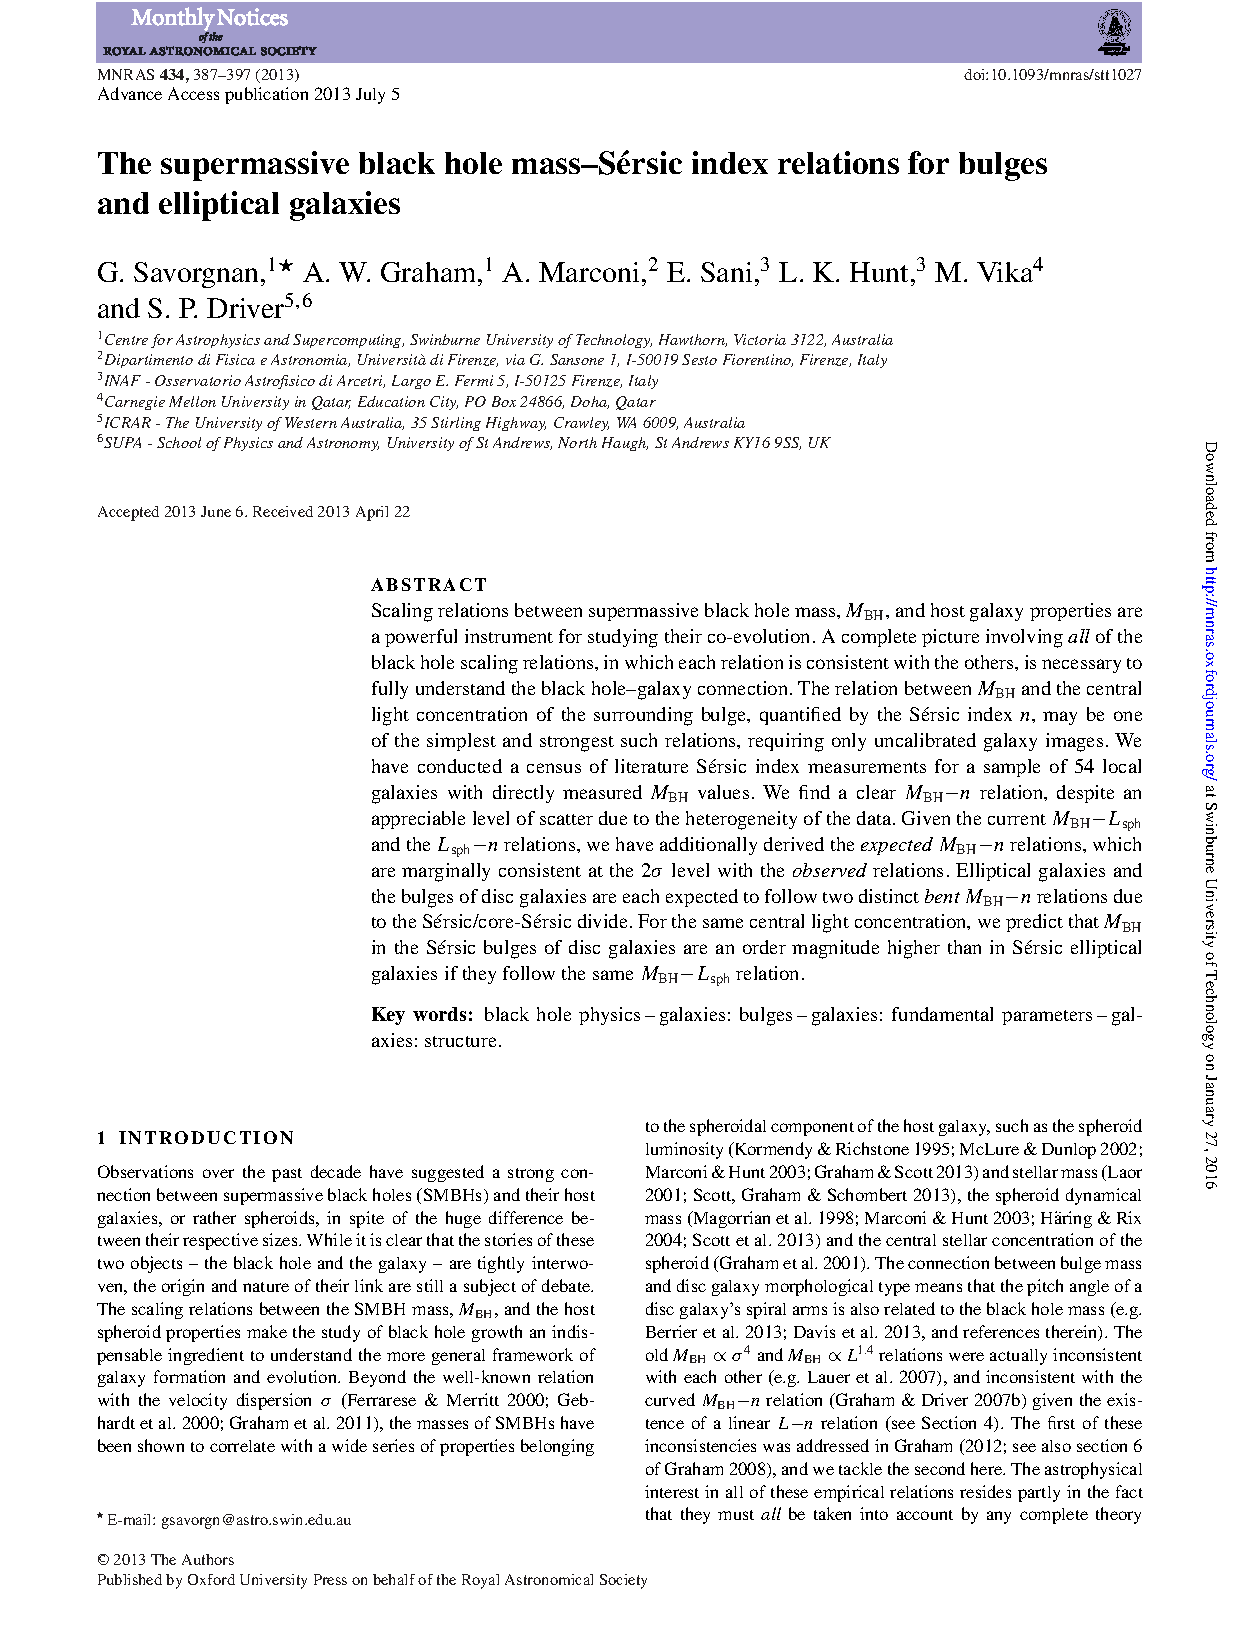
\includepdf[pages={1-11}]{MNRAS2013.pdf}


\chapter{Galaxy Vivisection}
\label{ch:galviv}

The preliminary investigation presented in Chapter \ref{ch:recov-mn} \citep{savorgnan2013} 
demonstrated the need for a new, systematic and homogeneous study 
aimed at obtaining more accurate galaxy decompositions 
and refining our knowledge about black hole mass scaling relations. 
In 2013, I visited A.~Marconi, E.~Sani, and L.~K.~Hunt (co-authors of the paper \citealt{sani2011}) 
in Arcetri (Florence) for a short collaboration, 
during which I was shown their 2D galaxy decomposition method using {\tt GALFIT3} \citep{peng2010}. 
This helped set the basis for the development of my own galaxy decomposition strategy. \\

Building on the catalog of \cite{grahamscott2013} 
with the addition of some new black hole mass measurements later published by \cite{rusli2013bhmassesDM}, 
I assembled my initial sample of 75 galaxies. 
For the imaging data, 
I chose to use \emph{Spitzer} archival observations at $3.6~\mu \rm m$ for three main reasons: 
(\emph{i}) the $3.6~\mu \rm m$ passband is currently the best proxy for the stellar mass 
(\citealt{sheth2010}, and references therein); 
(\emph{ii}) archival observations were publicly available for the majority of the galaxies in my initial sample; 
and (\emph{iii}) within a \emph{Spitzer} observation set of a galaxy, 
roughly half of the telescope pointings are dedicated to the imaging of the surrounding sky, 
ensuring a robust background determination during the data reduction process\footnote{These three points put together 
led me to prefer \emph{Spitzer} rather than \emph{HST} observations, 
albeit the lower spatial resolution. }. 
While for each galaxy \cite{sani2011} used only one set of \emph{Spitzer} astronomical observations, 
I downloaded all the publicly available observation sets and merged them into a single mosaic with higher signal-to-noise. 
I paid particular attention to (and invested a consistent amount of time into) the characterisation of the 
2D Point Spread Function (PSF), following the expert advice of C.~Peng. \\

Being aware of the importance of choosing the correct galaxy model 
in order to obtain reliable and meaningful structural parameters, 
I embraced the approach of \cite{laurikainen2005} 
and planned \emph{a priori} identification of the number and nature of the structural components in each galaxy. 
Given the lack of reference literature about advantages and disadvantages 
related to 1D and 2D decomposition techniques, 
I decided to experiment with both. \\ 

I wrote substantial software to perform 1D decomposition of surface brightness profiles. 
This code is written in {\tt Python} and is based on the Levenberg-Marquardt minimisation routine 
of the {\tt scipy.optimize} module. 
This software allows the user to build a galaxy model with any arbitrary number of analytical functions 
(S\'ersic, exponential, Gaussian, Ferrer, etc.). 
Because the code is written in an object-oriented fashion, 
it is particularly easy to implement any new analytical function into it. \\ 

For the 2D analysis, I experimented with the codes {\tt GALFIT3} \citep{peng2010} 
and {\tt Imfit} \citep{imfit}. 
After checking that both codes give consistent results, 
I preferred the more script-oriented {\tt Imfit} over {\tt GALFIT3}. \\ 

The NASA/IPAC Extragalactic Database (NED) has been an invaluable resource 
for the structural analysis of galaxies. 
NED lists all the literature references contained in the SAO/NASA Astrophysics Data System (ADS) 
which mentioned a particular galaxy. 
Thanks to this functionality, 
I was able to search for previous photometric and kinematic analyses, 
structural decompositions, information about the nuclear activity, 
presence of dust or peculiar features, 
and any other detail that could be useful to the analysis of my galaxies. \\

The remainder of this chapter comprises the published version of the paper 
``Supermassive Black Holes and Their Host Spheroids. I. Disassembling Galaxies'' 
by G.~A.~D.~Savorgnan \& A.~W.~Graham,  
as it appears in Volume 222 of the \emph{The Astrophysical Journal Supplement Series}. 


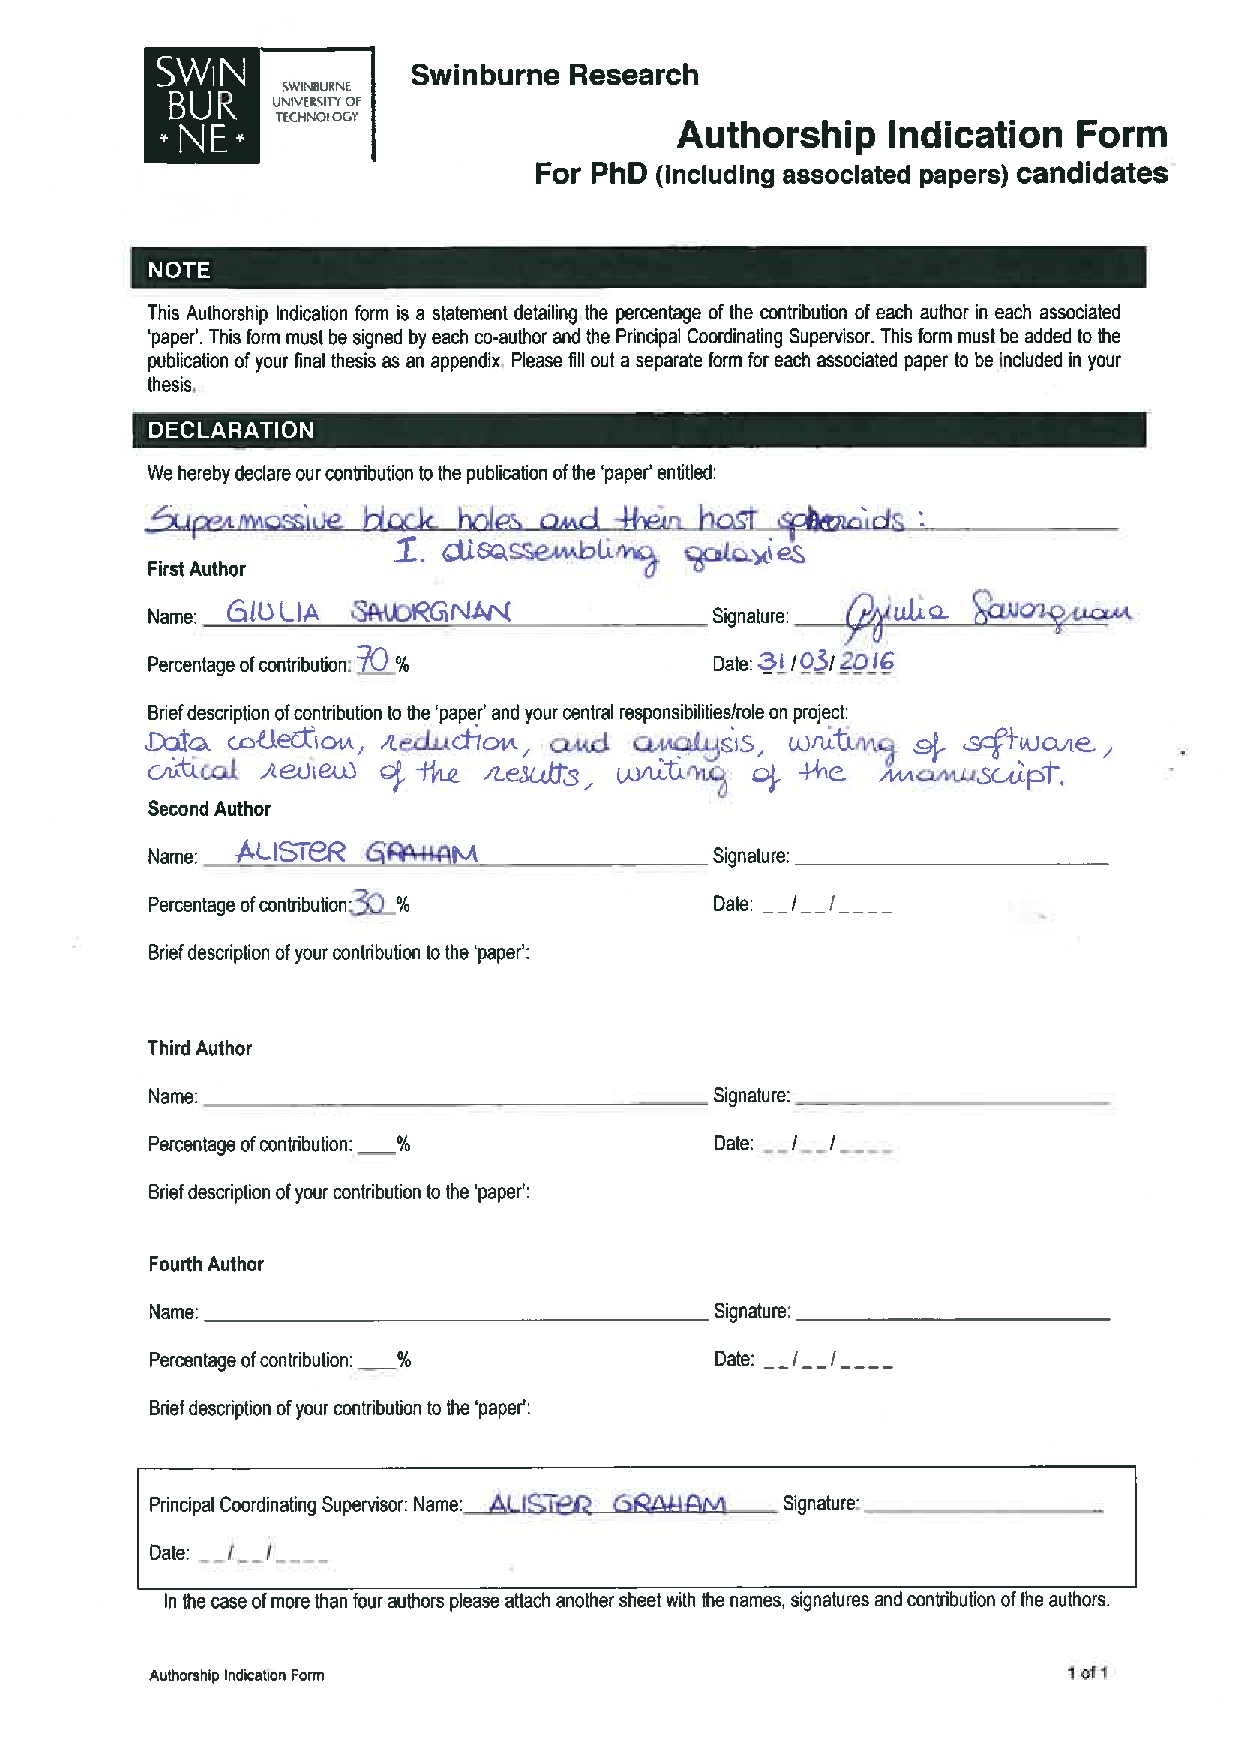
\includepdf[pages={1-58}]{ApJS2016.pdf}



\documentclass[preprint2]{emulateapj}

\usepackage{natbib}
\bibliographystyle{apj}
\usepackage{longtable}
\usepackage[]{graphicx}
\usepackage{amsmath}
\usepackage{natbib}
\usepackage{tabularx}
\usepackage{bm}
\usepackage{color}
\usepackage{hyperref}

%% Sometimes a paper's abstract is too long to fit on the
%% title page in preprint2 mode. When that is the case,
%% use the longabstract style option.

%% \documentclass[preprint2,longabstract]{aastex}

\newcommand{\vdag}{(v)^\dagger}
\newcommand{\myemail}{gsavorgn@astro.swin.edu.au}
\newcommand{\fitfigurewidth}{0.8\textwidth}


%\shorttitle{Early and late $M_{\rm BH} - M_{\rm *,sph}$ sequence}
\shorttitle{Red and blue $M_{\rm BH} - M_{\rm *,sph}$ sequence}

\shortauthors{Savorgnan et al.}

\begin{document}

%\title{Supermassive black hole and host bulge affairs \\ II. The early and late sequence in the $M_{\rm BH} - M_{\rm *,sph}$ diagram}
\title{Supermassive black hole and host spheroid affairs \\ II. The red and blue sequence in the $M_{\rm BH} - M_{\rm *,sph}$ diagram}

%\author{G. A. D. Savorgnan\altaffilmark{1} and A. W. Graham\altaffilmark{1} and A. Marconi and E. Sani\altaffilmark{3} and L.K. Hunt}
%\affil{Centre for Astrophysics and Supercomputing, Swinburne University of Technology, Hawthorn, Victoria 3122, Australia.}
%\email{gsavorgn@astro.swin.edu.au}


\author{Giulia A.~D.~Savorgnan and Alister W.~Graham}
\affil{Centre for Astrophysics and Supercomputing, Swinburne University of Technology, Hawthorn, Victoria 3122, Australia.}
\email{gsavorgn@astro.swin.edu.au}
\author{Alessandro Marconi}
\affil{Dipartimento di Fisica e Astronomia, Universit\'a di Firenze, via G. Sansone 1, I-50019 Sesto Fiorentino, Firenze, Italy.}
\and
\author{Eleonora Sani}
\affil{European Southern Observatory, Alonso de Cordova, Vitacura 3107, Santiago, Chile.}

%\and

%\author{A. W. Graham\altaffilmark{1}}
%\affil{Centre for Astrophysics and Supercomputing, Swinburne University of Technology, Hawthorn, Victoria 3122, Australia.}

%% Notice that each of these authors has alternate affiliations, which
%% are identified by the \altaffilmark after each name.  Specify alternate
%% affiliation information with \altaffiltext, with one command per each
%% affiliation.

%\altaffiltext{1}{}
%\altaffiltext{2}{Society of Fellows, Harvard University.}
%\altaffiltext{3}{present address: Center for Astrophysics,
%    60 Garden Street, Cambridge, MA 02138}
%\altaffiltext{4}{Visiting Programmer, Space Telescope Science Institute}
%\altaffiltext{5}{Patron, Alonso's Bar and Grill}

%% Mark off your abstract in the ``abstract'' environment. In the manuscript
%% style, abstract will output a Received/Accepted line after the
%% title and affiliation information. No date will appear since the author
%% does not have this information. The dates will be filled in by the
%% editorial office after submission.

\begin{abstract}
In our first paper, we performed a detailed (i.e.~bulge, disks, bars, spiral arms, rings, halo, nucleus, etc.) 
decomposition of 66 galaxies, with directly measured black hole masses, 
that had been imaged at $3.6\rm~\mu m$ with \emph{Spitzer}.
Our sample is the largest to date and, for the first time, the decompositions were checked for consistency with the galaxy kinematics. 
We present correlations between the black hole mass, $M_{\rm BH}$, 
and the host spheroid (and galaxy) luminosity, $L_{\rm sph}$ (and $L_{\rm gal}$), 
and also stellar mass, $M_{\rm *,sph}$.
Most previous studies have used galaxy samples that were overwhelmingly dominated by high-mass, early-type galaxies.
Instead, our sample includes 17 spiral galaxies, half of which have $M_{\rm BH} < 10^7\rm~M_\odot$, 
and allows us to better investigate the poorly studied low-mass end of the $M_{\rm BH} - M_{\rm *,sph}$ correlation.
The bulges of early-type (E + S0) galaxies follow $M_{\rm BH} \propto M_{\rm *,sph}^{1.04 \pm 0.10}$  
and define a tight %\emph{early-type sequence} 
\emph{red sequence} with intrinsic scatter $\epsilon_{(Y|X)} = 0.43 \pm 0.06\rm~dex$ 
and a median $M_{\rm BH}/M_{\rm *,sph}$ ratio of $0.68 \pm 0.04\%$, 
i.e.~a $\pm 2\sigma$ range of 0.1--5\%.
At the low-mass end, the bulges of late-type (Sp) galaxies define a much steeper %\emph{late-type sequence}, 
\emph{blue sequence}, 
with $M_{\rm BH} \propto M_{\rm *,sph}^{2-3}$, 
indicating that gas-rich processes feed the black hole more efficiently than the host bulge as they coevolve. 
We additionally report that: i) S\'ersic galaxies follow $M_{\rm BH} \propto M_{\rm *,sph}^{1.48 \pm 0.20}$, a less steep sequence than previously reported; 
ii) bulges with S\'ersic index $n_{\rm sph}<2$, argued by some to be pseudo-bulges, 
are not offset to lower $M_{\rm BH}$ from the correlation defined by the current bulge sample with $n_{\rm sph}>2$; 
and iii) $L_{\rm sph}$ and $L_{\rm gal}$ correlate equally well with $M_{\rm BH}$, in terms of intrinsic scatter, only for early-type galaxies 
(most elliptical galaxies contain disks, i.e.~$L_{\rm sph} \neq L_{\rm gal}$) --
once reasonable numbers of spiral galaxies are included, the correlation with $L_{\rm sph}$ is better than that with $L_{\rm gal}$. 

\end{abstract}

\keywords{black hole physics; galaxies: bulges; galaxies: elliptical and lenticular, cD; galaxies: evolution; galaxies: structure}

\section{Introduction}
\label{sec:int}
A quarter of a century ago, 
\cite{dressler1989} foresaw a ``rough scaling of black hole mass with the mass of the spheroidal component'' of galaxies, 
as suggested by the sequence of five galaxies (M87, M104, M31, M32 and the Milky Way). 
\cite{yee1992} then announced a linear relation between what was effectively black hole mass and galaxy mass for high-luminosity, bulge-dominated early-type galaxies 
radiating near the Eddington limit.
This ``rough scaling'' was a premature version of the early correlations between black hole mass, $M_{\rm BH}$,  
and host spheroid luminosity, $L_{\rm sph}$, and also host spheroid mass, $M_{\rm sph}$ 
\citep{kormendyrichstone1995,magorrian1998,marconihunt2003,haringrix2004}. 
These initial studies were dominated by high-mass, early-type galaxies, 
for which they too reported a quasi-linear $M_{\rm BH} - M_{\rm sph}$ relation. 
Subsequent studies of the $M_{\rm BH} - L_{\rm sph}$ and $M_{\rm BH} - M_{\rm sph}$ diagrams 
(\citealt{ferrareseford2005,lauer2007,graham2007,gultelkin2009,sani2011,beifiori2012,erwingadotti2012,
vika2012,vandenbosch2012,mcconnellma2013,kormendyho2013})
continued to use galaxy samples dominated by high-mass, early-type systems with $M_{\rm BH} \gtrsim 0.5 \times 10^8~\rm M_\odot$, 
and they too recovered a near-linear relation. 
However, the consensus about a linear $M_{\rm BH} - M_{\rm sph}$ correlation was not unanimous. 
Some studies had reported a slope steeper than one,  
or noticed that the low-mass spheroids were offset to the right of (or below) the relation traced by the high-mass spheroids 
\citep{laor1998,wandel1999,laor2001,ryan2007}.
\cite{graham2012bent}, \cite{grahamscott2013} and \cite{scott2013} found two distinct trends in the $M_{\rm BH} - L_{\rm sph}$ and $M_{\rm BH} - M_{\rm sph}$ diagrams:  
a linear and a super-quadratic correlation at the high- and low-mass end, respectively\footnote{Readers 
interested in an extensive review about the early discovery and successive improvements of these correlations 
should consult \cite{graham2015bulges}.}. \\
Recently, \cite{lasker2014data,lasker2014anal} derived $2.2~\rm \mu m$ bulge luminosities for 35 galaxies 
(among which only 4 were classified as spiral galaxies), 
and reported a slope below unity for their $M_{\rm BH} - L_{\rm sph}$ relation. 
They also claimed that the black hole mass correlates equally well with the total galaxy luminosity 
as it does with the bulge luminosity.  \\
The $M_{\rm BH} - L_{\rm sph}$ relation for early-type (elliptical + lenticular) galaxies can be predicted by combining two other correlations that involve 
the bulge stellar velocity dispersion, $\sigma$.
One of these is the $M_{\rm BH} - \sigma$ relation \citep{ferraresemerritt2000,gebhardt2000},
which can be described with a single power-law ($M_{\rm BH} \propto \sigma^{5-6}$) 
over a wide range in velocity dispersion ($70-350~\rm km~s^{-1}$, e.g.~\citealt{graham2011,mcconnell2011,grahamscott2013}).
The other is the $L_{\rm sph} - \sigma$ relation, 
which has long been known to be a ``double power-law'', 
with $L_{\rm sph} \propto \sigma^{5-6}$ at the luminous end\footnote{Recent 
work has the $M_{\rm BH} - \sigma$ correlation as steep as $M_{\rm BH} \propto \sigma^{6.5}$ \citep{savorgnangraham2015},
and the high-luminosity end of the $L_{\rm sph} - \sigma$ correlation as steep as $L_{\rm sph} \propto \sigma^{8}$ \citep{monterodorta2015}.} 
\citep{schechter1980,malumuthkrishner1981,vonderlinden2007,lauer2007lumell,liu2008}
and $L_{\rm sph} \propto \sigma^2$ at intermediate and faint luminosities 
\citep{davies1983,held1992,matkovicguzman2005,derijcke2005,balcells2007screl,chilingarian2008,forbes2008,cody2009,tortora2009,kourkchi2012}. 
The change in slope of the $L_{\rm sph} - \sigma$ relation occurs at $M_B \approx -20.5\rm~mag$, 
corresponding to $\sigma \approx 200~\rm km~s^{-1}$. 
The $M_{\rm BH} - L_{\rm sph}$ relation should therefore be better described by a ``broken'', rather than a single power-law: 
with $M_{\rm BH} \propto L_{\rm sph}^{2.5}$ at the low-luminosity end, 
and $M_{\rm BH} \propto L_{\rm sph}^1$ at the high-luminosity end.  
Due to the scatter in the $M_{\rm BH} - L_{\rm sph}$ (or $M_{\rm BH} - M_{\rm sph}$) diagram, 
studies that have not sufficiently probed below $M_{\rm BH} \approx 10^7\rm~M_\odot$ 
can easily miss the change in slope occuring at $M_{\rm BH} \approx 10^{(8 \pm 1)}\rm~M_\odot$, 
and erroneously recover a single log-linear relation. \\
When \cite{graham2012bent} pointed out this overlooked inconsistency between these linear and bent relations, 
he identified two different populations of galaxies, 
namely the core-S\'ersic spheroids \citep{graham2003coresersicmodel,trujillo2004coresersicmodel} and the S\'ersic 
spheroids\footnote{Core-S\'ersic spheroids have partially depleted cores relative to their outer S\'ersic light profile, 
whereas S\'ersic spheroids have no central deficit of stars.},
and attributed the change in slope (from super-quadratic to linear) to their different formation mechanisms. 
In this scenario, core-S\'ersic spheroids are built in dry merger events 
where the black hole and the bulge grow at the same pace, increasing their mass in lock steps ($M_{\rm BH} \propto L_{\rm sph}^1$), 
whereas S\'ersic spheroids originate from gas-rich processes 
in which the mass of the black hole increases more rapidly than the mass of its host spheroid ($M_{\rm BH} \propto L_{\rm sph}^{2.5}$). \\
\citeauthor{grahamscott2013} (\citeyear{grahamscott2013}, hereafter GS13) and \citeauthor{scott2013} (\citeyear{scott2013}) 
presented separate power-law linear regressions 
for the S\'ersic and core-S\'ersic spheroids in the $M_{\rm BH} - L_{\rm sph}$ and $M_{\rm BH} - M_{\rm *,sph}$ 
(spheroid stellar mass) diagrams, probing down to $M_{\rm BH} \approx 10^6\rm~M_\odot$. 
To obtain their dust-corrected \emph{bulge} magnitudes, they did not perform bulge/disc decompositions, 
but converted the $B-$band and $K_S-$band observed, total \emph{galaxy} magnitudes into bulge magnitudes 
using a mean statistical bulge-to-total ratio based on each object's morphological type and disc 
inclination\footnote{While this resulted in individual bulge magnitudes not being exactly correct, 
their large sample size allowed them to obtain a reasonable $M_{\rm BH} - L_{\rm sph}$ relation for the ensemble.}. 
These mean statistical bulge-to-total ratios were obtained from the results of two-component (S\'ersic-bulge/exponential-disk) decompositions in the literature. \\
%It should also be noted that $\sim$80\% of their core-S\'ersic spheroids were morphologically classified as elliptical galaxies, 
%and $\sim$80\% of their S\'ersic spheroids were morphologically classified as bulges of disk galaxies (lenticulars and spirals). \\
%Several recent papers \citep{jiang2011a,jiang2013,mathur2012,reines2013} claimed an offset at the low-mass end of the $M_{\rm BH} - M_{\rm *,sph}$ diagram,
%such that the black hole mass is lower than expected from the near-linear correlation traced by the high-mass, early-type spheroids. 
%However, \cite{grahamscott2013} showed that the low-mass spheroids ($10^{8.5} \lesssim M_{\rm *,sph}/{\rm M_\odot} \lesssim 10^{10.5}$) 
%are not randomly offset from such near-linear correlation, 
%but follow the steeper relation traced by the S\'ersic spheroids. 
%Using bulge/disk decomposition data from \cite{jiang2011a}, 
%\cite{grahamscott2015} derived the host spheroid masses 
%and showed that the steeper $M_{\rm BH} - M_{\rm *,sph}$ extends to these spheroids with even lower black hole masses 
%($10^{5} \lesssim M_{\rm *,sph}/{\rm M_\odot} \lesssim 2 \times 10^{6}$), 
%and a more detailed analysis will be presented in Graham et al. (2015, \emph{in preparation}).  \\
Here we investigate in more detail %substructure in 
the $M_{\rm BH} - L_{\rm sph}$ and $M_{\rm BH} - M_{\rm *,sph}$ diagrams 
using state-of-the-art galaxy decompositions (Savorgnan \& Graham 2015, hereafter \emph{Paper I}) 
for galaxies with directly measured black hole masses.
Our galaxies are large and nearby, which allows us to perform accurate multicomponent decompositions 
(instead of simple bulge/disk decompositions). 
Our decompositions were performed on $3.6\rm~\mu m$ \emph{Spitzer} satellite imagery, 
which is an excellent proxy for the stellar mass, superior to the $K-$band (\citealt{sheth2010}, and references therein).
Nine of our galaxies have $M_{\rm BH} \lesssim 10^7\rm~M_\odot$, 
which allows us to better constrain the slope of the correlation at the low-mass end.
Furthermore, our galaxy sample includes 17 spiral galaxies, 
representing a notable improvement over past studies dominated by early-type galaxies. 
In a forthcoming paper, we will explore the relation between the black hole mass and the bulge dynamical mass, 
$M_{\rm dyn,sph} \propto R_{\rm e} \sigma^2$, and address the issue of a black hole fundamental plane.
%{\bf This paper is structured as follows... }

\section{Data}
\label{sec:data}
Our galaxy sample (see Table \ref{tab:sample}) 
consists of 66 objects for which a dynamical measurement of the black hole mass had been tabulated in the literature 
(by GS13 or \citealt{rusli2013bhmassesDM}) at the time that we started this project, 
and for which we were able to obtain useful spheroid parameters from $3.6\rm~\mu m$ \emph{Spitzer} satellite imagery. \\
Spheroid magnitudes were derived from our state-of-the-art galaxy decompositions, which take into account 
bulge, disks, spiral arms, bars, rings, halo, extended or unresolved nuclear source and partially depleted core. 
Kinematical information \citep{atlas3dIII-MNRAS,scott2014,arnold2014} was used 
to confirm the presence of rotationally supported disk components in most early-type (elliptical + lenticular) galaxies, 
and to identify their extent 
(intermediate-scale disks that are fully embedded in the bulge, 
or large-scale disks that encase the bulge and dominate the light at large radii). 
It is worth stressing that, contrary to common knowledge, the majority of ``elliptical'' galaxies contain disks,
i.e.~they are not single-component spheroidal systems.
\emph{Paper I} presents the dataset used here, 
%to investigate the $M_{\rm BH} - L_{\rm gal}$, $M_{\rm BH} - L_{\rm sph}$ and $M_{\rm BH} - M_{\rm *,sph}$ diagrams, 
including details about the data reduction process and the galaxy modelling technique that we developed. 
It also discusses how we estimated the uncertainties\footnote{By comparing, for each of our galaxies, the measurements of the bulge magnitude 
obtained by different authors with that obtained by us, we estimated the uncertainties on the bulge magnitudes, 
in effect taking into account systematic errors. 
Systematic errors include incorrect sky subtraction, inaccurate masking of contaminating sources, imprecise description of the PSF, 
erroneous choice of model components (for example, when failing to identify a galaxy subcomponent and thus omitting it in the model, 
or when describing a galaxy sub-component with an inadequate function), 
the radial extent of the surface brightness profile and one's sampling of this. 
Most of these factors are not included in popular 2D fitting codes which report only the {\bf statistical} errors associated with their fitted parameters. 
In fact, when performing multi-component decomposition of high signal-to-noise images of nearby -- therefore well spatially resolved -- galaxies, 
errors are dominated by systematics rather than Poisson noise.} 
on the bulge magnitudes, and presents the individual 66 galaxy decompositions, 
along with a comparison and discussion of past decompositions. \\
Bulge luminosities\footnote{Following \cite{sani2011}, absolute luminosities were calculated 
assuming a $3.6\rm~\mu m$ solar absolute magnitude of $3.25\rm~mag$. 
Absolute luminosities were not corrected for cosmological redshift dimming 
(this correction would be as small as $-0.02\rm~mag$ for galaxies at a distance of $40\rm~Mpc$ 
or $-0.05\rm~mag$ for galaxies at a distance of $100\rm~Mpc$).} 
(Table \ref{tab:sample}) from \emph{Paper I} were converted into stellar masses 
using a constant $3.6\rm~\mu m$ mass-to-light ratio, $\Gamma_{3.6} = 0.6$ \citep{meidt2014}.
We additionally explored a more sophisticated way to compute mass-to-light ratios, 
using the color-$\Gamma_{3.6}$ relation published by 
\citeauthor{meidt2014} (\citeyear{meidt2014}, their equation 4), 
which allows one to estimate $\Gamma_{3.6}$ of a galaxy from its $[3.6] - [4.5]$ color. 
Individual $[3.6] - [4.5]$ colors\footnote{These are integrated $[3.6] - [4.5]$ colors, measured in a circular aperture 
within each galaxy's effective radius.} were taken from 
\citeauthor{peletier2012} (\citeyear{peletier2012}, column 8 of their Table 1) 
when available for our galaxies, 
or were estimated from the bulge stellar velocity dispersion, $\sigma$, 
using the color-$\sigma$ relation presented by \citeauthor{peletier2012} (\citeyear{peletier2012}, their Figure 6).
We found that the range in $[3.6] - [4.5]$ color is small ($0.06\rm~mag$), 
and thus the range in $\Gamma_{3.6}$ is also small ($0.04$).
After checking that using a single $\Gamma_{3.6} = 0.6$, independent of $[3.6] - [4.5]$ color, 
does not significantly affect the results of our analysis, 
we decided to use individual, color-dependent mass-to-light ratios. \\
For each galaxy, the total luminosity (or galaxy luminosity, $L_{\rm gal}$) is the sum of the luminosities of all its sub-components. 
Due to the complexity of their modelling, 
four galaxies (see Table \ref{tab:sample}, column 7) had their galaxy luminosities 
underestimated\footnote{These four cases are discussed in \emph{Paper I}.}, 
which are given here as lower limits. 
Following GS13, we assumed a fixed uncertainty ($0.25\rm~mag$) for the absolute galaxy magnitude $MAG_{\rm gal}$. \\
The morphological classification (E = elliptical; E/S0 = elliptical/lenticular; S0 = lenticular; S0/Sp = lenticular/spiral; Sp = spiral; and ``merger'') 
follows from the galaxy models presented in \emph{Paper I}. 
Throughout this paper we will refer to early-type galaxies (E+S0) and late-type galaxies (Sp). 
Two galaxies classified as E/S0 are obviously included in the early-type bin, 
whereas two galaxies classified as S0/Sp and another two classified as mergers are included in neither the early- nor the late-type bin.\\
The S\'ersic/core-S\'ersic classification presented in this work 
comes from the compilation of \citet{savorgnangraham2015},
who identified partially depleted cores according to the same criteria used by GS13.
When no high-resolution image analysis was available from the literature, 
they inferred the presence of a partially depleted core based on the stellar velocity dispersion:
a spheroid is classified as core-S\'ersic if $\sigma > 270\rm~km~s^{-1}$,
or as S\'ersic if $\sigma < 166\rm~km~s^{-1}$. 
All of the galaxies with velocity dispersions between these two limits had high-resolution images available. 

\begin{table*}                                        
\begin{center}                                        
\caption{{\bf Galaxy sample.}                        
\emph{Column (1):} Galaxy name.                       
\emph{Column (2):} Distance.                                   
\emph{Column (3):} Black hole mass.                                   
\emph{Column (4):} Reference of the black hole mass reported here (G+03 = \citealt{greenhill2003}, GS13 = \citealt{grahamscott2013}; R+13b = \citealt{rusli2013bhmassesDM}).                                   
\emph{Column (5):} Presence of a partially depleted core. 
The question mark is used when the classification has come from the velocity dispersion criteria mentioned in Section \ref{sec:corser}. 
The value of the core break radius is reported in parenthesis when available.  
\emph{Column (6):} Reference of the identification of a partially depleted core (G+94 = \citealt{grillmair1994}; F+97 = \citealt{forbes1997}; Q+00 = \citealt{quillen2000}, 
T+04 = \citealt{trujillo2004coresersicmodel}; F+06 = \citealt{ferrarese2006acsvcs}; J+11 = \citealt{jardel2011}; R+11 = \citealt{richings2011}; 
DG13 = \citealt{dullograham2013cores}; R+13a = \citealt{rusli2013}).  
\emph{Column (7):} Kinematical classification (fast/slow rotator).
\emph{Column (8):} Availability of velocity map (A = ATLAS$^{\rm 3D}$, S = SLUGGS). 
\emph{Column (9):} Completion of 1D fit. 
\emph{Column (10):} Completion of 2D fit. }                                 
\begin{tabular}{llllllllll}                           
\hline                                                
\multicolumn{1}{l}{{\bf Galaxy}} &                   
\multicolumn{1}{l}{{\bf Distance}} &                 
\multicolumn{1}{l}{{\bf $\bm{M_{\rm BH}}$}} &  
\multicolumn{1}{l}{{\bf Ref.}} &                     
\multicolumn{1}{l}{{\bf Core}} &                     
\multicolumn{1}{l}{{\bf Ref.}} &                     
\multicolumn{1}{l}{{\bf Rot.}} &                     
\multicolumn{1}{l}{{\bf Vel. map}} &                 
\multicolumn{1}{l}{{\bf 1D fit}} &                   
\multicolumn{1}{l}{{\bf 2D fit}} \\                
\multicolumn{1}{l}{} &                                
\multicolumn{1}{l}{[Mpc]} &                           
\multicolumn{1}{l}{$[10^8~\rm M_{\odot}]$} &         
\multicolumn{1}{l}{} &                                
\multicolumn{1}{l}{$([\rm arcsec])$} &                                
\multicolumn{1}{l}{} &                                
\multicolumn{1}{l}{} &                                
\multicolumn{1}{l}{} &                                
\multicolumn{1}{l}{} &                                
\multicolumn{1}{l}{} \\                             
\multicolumn{1}{l}{(1)} &                             
\multicolumn{1}{l}{(2)} &                             
\multicolumn{1}{l}{(3)} &                             
\multicolumn{1}{l}{(4)} &                             
\multicolumn{1}{l}{(5)} &                             
\multicolumn{1}{l}{(6)} &                             
\multicolumn{1}{l}{(7)} &                             
\multicolumn{1}{l}{(8)} &                             
\multicolumn{1}{l}{(9)} &                             
\multicolumn{1}{l}{(10)} \\                         
\hline                                                
Circinus   &  $4.0$  &  $0.017_{-0.003}^{+0.004}$   &  G+03  &  no?  &     &      &     &  no  &  no  \\ 
IC 1459  &  $28.4$  &  $24_{-10}^{+10}$   &  GS13  &  yes  $(0.7)$  &  R+13a  &      &     &  yes  &  yes  \\ 
IC 2560  &  $40.7$  &  $0.044_{-0.022}^{+0.044}$   &  GS13  &  no?  &     &      &     &  yes  &  no  \\ 
IC 4296  &  $40.7$  &  $11_{-2}^{+2}$   &  GS13  &  yes?  &     &      &     &  yes  &  yes  \\ 
M104  &  $9.5$  &  $6.4_{-0.4}^{+0.4}$   &  GS13  &  yes   &  J+11  &      &     &  yes  &  no  \\ 
M105  &  $10.3$  &  $4_{-1}^{+1}$   &  GS13  &  yes  $(1.1)$  &  DG13, R+13a  &  FAST   &  A  &  yes  &  yes  \\ 
M106  &  $7.2$  &  $0.39_{-0.01}^{+0.01}$   &  GS13  &  no   &     &      &     &  yes  &  no  \\ 
M31  &  $0.7$  &  $1.4_{-0.3}^{+0.9}$   &  GS13  &  no   &     &      &     &  yes  &  no  \\ 
M32  &  $0.8$  &  $0.024_{-0.005}^{+0.005}$   &  GS13  &  no   &     &      &     &  no  &  no  \\ 
M49  &  $17.1$  &  $25_{-1}^{+3}$   &  R+13b  &  yes  $(1.5)$  &  DG13, R+13a  &   SLOW  &  A  &  yes  &  yes  \\ 
M59  &  $17.8$  &  $3.9_{-0.4}^{+0.4}$   &  GS13  &  no   &     &  FAST   &  A  &  yes  &  no  \\ 
M60  &  $16.4$  &  $47_{-10}^{+10}$   &  GS13  &  yes  $(2.7)$  &  DG13, R+13a  &  FAST   &  A, S  &  no  &  no  \\ 
M64  &  $7.3$  &  $0.016_{-0.004}^{+0.004}$   &  GS13  &  no?  &     &      &     &  yes  &  no  \\ 
M77  &  $15.2$  &  $0.084_{-0.003}^{+0.003}$   &  GS13  &  no   &     &      &     &  no  &  no  \\ 
M81  &  $3.8$  &  $0.74_{-0.11}^{+0.21}$   &  GS13  &  no   &     &      &     &  yes  &  no  \\ 
M84  &  $17.9$  &  $9.0_{-0.8}^{+0.9}$   &  GS13  &  yes  $(1.9)$  &  F+06  &   SLOW  &  A, S  &  yes  &  yes  \\ 
M87  &  $15.6$  &  $58.0_{-3.5}^{+3.5}$   &  GS13  &  yes  $(7.2)$  &  F+06  &   SLOW  &  A, S  &  yes  &  yes  \\ 
M89  &  $14.9$  &  $4.7_{-0.5}^{+0.5}$   &  GS13  &  yes  $(0.4)$  &  DG13, R+13a  &   SLOW  &  A  &  yes  &  no  \\ 
M94  &  $4.4$  &  $0.060_{-0.014}^{+0.014}$   &  GS13  &  no?  &     &      &     &  yes  &  no  \\ 
M96  &  $10.1$  &  $0.073_{-0.015}^{+0.015}$   &  GS13  &  no   &     &      &     &  yes  &  yes  \\ 
NGC 0253  &  $3.5$  &  $0.10_{-0.05}^{+0.10}$   &  GS13  &  no   &     &      &     &  no  &  no  \\ 
NGC 0524  &  $23.3$  &  $8.3_{-1.3}^{+2.7}$   &  GS13  &  yes  $(0.2)$  &  R+11  &  FAST   &  A  &  yes  &  no  \\ 
NGC 0821  &  $23.4$  &  $0.39_{-0.09}^{+0.26}$   &  GS13  &  no   &     &  FAST   &  A, S  &  yes  &  yes  \\ 
NGC 1023  &  $11.1$  &  $0.42_{-0.04}^{+0.04}$   &  GS13  &  no   &     &  FAST   &  A, S  &  yes  &  yes  \\ 
NGC 1300  &  $20.7$  &  $0.73_{-0.35}^{+0.69}$   &  GS13  &  no   &     &      &     &  yes  &  no  \\ 
NGC 1316  &  $18.6$  &  $1.50_{-0.80}^{+0.75}$   &  GS13  &  no   &     &  FAST   &     &  yes  &  no  \\ 
NGC 1332  &  $22.3$  &  $14_{-2}^{+2}$   &  GS13  &  no   &     &      &     &  yes  &  no  \\ 
NGC 1374  &  $19.2$  &  $5.8_{-0.5}^{+0.5}$   &  R+13b  &  no?  &     &  FAST   &  A  &  yes  &  yes  \\ 
NGC 1399  &  $19.4$  &  $4.7_{-0.6}^{+0.6}$   &  GS13  &  yes  $(2.4)$  &  DG13, R+13a  &   SLOW  &  A  &  yes  &  no  \\ 
NGC 2273  &  $28.5$  &  $0.083_{-0.004}^{+0.004}$   &  GS13  &  no   &     &      &     &  yes  &  no  \\ 
NGC 2549  &  $12.3$  &  $0.14_{-0.13}^{+0.02}$   &  GS13  &  no   &     &  FAST   &  A  &  yes  &  yes  \\ 
NGC 2778  &  $22.3$  &  $0.15_{-0.10}^{+0.09}$   &  GS13  &  no   &     &  FAST   &  A  &  yes  &  no  \\ 
NGC 2787  &  $7.3$  &  $0.40_{-0.05}^{+0.04}$   &  GS13  &  no   &     &      &     &  yes  &  no  \\ 
NGC 2974  &  $20.9$  &  $1.7_{-0.2}^{+0.2}$   &  GS13  &  no   &     &  FAST   &  A, S  &  yes  &  yes  \\ 
NGC 3079  &  $20.7$  &  $0.024_{-0.012}^{+0.024}$   &  GS13  &  no?  &     &      &     &  yes  &  no  \\ 
NGC 3091  &  $51.2$  &  $36_{-2}^{+1}$   &  R+13b  &  yes  $(0.6)$  &  R+13a  &      &     &  yes  &  yes  \\ 
NGC 3115  &  $9.4$  &  $8.8_{-2.7}^{+10.0}$   &  GS13  &  no   &     &      &     &  yes  &  no  \\ 
NGC 3227  &  $20.3$  &  $0.14_{-0.06}^{+0.10}$   &  GS13  &  no   &     &      &     &  yes  &  no  \\ 
NGC 3245  &  $20.3$  &  $2.0_{-0.5}^{+0.5}$   &  GS13  &  no   &     &  FAST   &  A  &  yes  &  yes  \\ 
NGC 3377  &  $10.9$  &  $0.77_{-0.06}^{+0.04}$   &  GS13  &  no   &     &  FAST   &  A, S  &  yes  &  yes  \\ 
NGC 3384  &  $11.3$  &  $0.17_{-0.02}^{+0.01}$   &  GS13  &  no   &     &  FAST   &  A  &  yes  &  no  \\ 
NGC 3393  &  $55.2$  &  $0.34_{-0.02}^{+0.02}$   &  GS13  &  no   &     &      &     &  yes  &  yes  \\ 
NGC 3414  &  $24.5$  &  $2.4_{-0.3}^{+0.3}$   &  GS13  &  no   &     &   SLOW  &  A  &  yes  &  no  \\ 
NGC 3489  &  $11.7$  &  $0.058_{-0.008}^{+0.008}$   &  GS13  &  no   &     &  FAST   &  A  &  yes  &  yes  \\ 
NGC 3585  &  $19.5$  &  $3.1_{-0.6}^{+1.4}$   &  GS13  &  no   &     &      &     &  yes  &  no  \\ 
NGC 3607  &  $22.2$  &  $1.3_{-0.5}^{+0.5}$   &  GS13  &  no   &     &  FAST   &  A  &  yes  &  yes  \\ 
NGC 3608  &  $22.3$  &  $2.0_{-0.6}^{+1.1}$   &  GS13  &  yes  $(0.2)$  &  DG13, R+13a  &   SLOW  &  A, S  &  yes  &  yes  \\ 
NGC 3842  &  $98.4$  &  $97_{-26}^{+30}$   &  GS13  &  yes  $(0.7)$  &  DG13, R+13a  &      &     &  yes  &  no  \\ 
NGC 3998  &  $13.7$  &  $8.1_{-1.9}^{+2.0}$   &  GS13  &  no   &     &  FAST   &  A  &  yes  &  no  \\ 
NGC 4026  &  $13.2$  &  $1.8_{-0.3}^{+0.6}$   &  GS13  &  no   &     &  FAST   &  A  &  yes  &  no  \\ 
NGC 4151  &  $20.0$  &  $0.65_{-0.07}^{+0.07}$   &  GS13  &  no   &     &      &     &  yes  &  no  \\ 
\hline         
\end{tabular}   
\label{tab:sample} 
\end{center}    
\end{table*}    

\begin{table*}                                        
\begin{center}                                        
\begin{tabular}{llllllllll}                           
\hline                                                
\multicolumn{1}{l}{{\bf Galaxy}} &                   
\multicolumn{1}{l}{{\bf Distance}} &                 
\multicolumn{1}{l}{{\bf $\mathbf{M_{\rm BH}}$}} &  
\multicolumn{1}{l}{{\bf Ref.}} &                     
\multicolumn{1}{l}{{\bf Core}} &                     
\multicolumn{1}{l}{{\bf Ref.}} &                     
\multicolumn{1}{l}{{\bf Rot.}} &                     
\multicolumn{1}{l}{{\bf Vel. map}} &                 
\multicolumn{1}{l}{{\bf 1D fit}} &                   
\multicolumn{1}{l}{{\bf 2D fit}} \\                
\multicolumn{1}{l}{} &                                
\multicolumn{1}{l}{[Mpc]} &                           
\multicolumn{1}{l}{$[10^8~\rm M_{\odot}]$} &         
\multicolumn{1}{l}{} &                                
\multicolumn{1}{l}{$([\rm arcsec])$} &                                
\multicolumn{1}{l}{} &                                
\multicolumn{1}{l}{} &                                
\multicolumn{1}{l}{} &                                
\multicolumn{1}{l}{} &                                
\multicolumn{1}{l}{} \\                             
\multicolumn{1}{l}{(1)} &                             
\multicolumn{1}{l}{(2)} &                             
\multicolumn{1}{l}{(3)} &                             
\multicolumn{1}{l}{(4)} &                             
\multicolumn{1}{l}{(5)} &                             
\multicolumn{1}{l}{(6)} &                             
\multicolumn{1}{l}{(7)} &                             
\multicolumn{1}{l}{(8)} &                             
\multicolumn{1}{l}{(9)} &                             
\multicolumn{1}{l}{(10)} \\                         
\hline                                                
NGC 4261  &  $30.8$  &  $5_{-1}^{+1}$   &  GS13  &  yes  $(1.6)$  &  R+11  &   SLOW  &  A  &  yes  &  yes  \\ 
NGC 4291  &  $25.5$  &  $3.3_{-2.5}^{+0.9}$   &  GS13  &  yes  $(0.3)$  &  DG13, R+13a  &      &     &  yes  &  yes  \\ 
NGC 4342  &  $23.0$  &  $4.5_{-1.5}^{+2.3}$   &  GS13  &  no   &     &  FAST   &  A  &  no  &  no  \\ 
NGC 4388  &  $17.0$  &  $0.075_{-0.002}^{+0.002}$   &  GS13  &  no?  &     &      &     &  yes  &  no  \\ 
NGC 4459  &  $15.7$  &  $0.68_{-0.13}^{+0.13}$   &  GS13  &  no   &     &  FAST   &  A  &  yes  &  no  \\ 
NGC 4473  &  $15.3$  &  $1.2_{-0.9}^{+0.4}$   &  GS13  &  no   &     &  FAST   &  A, S  &  yes  &  yes  \\ 
NGC 4486A  &  $17.0$  &  $0.13_{-0.08}^{+0.08}$   &  GS13  &  no   &     &  FAST   &  A  &  no  &  no  \\ 
NGC 4564  &  $14.6$  &  $0.60_{-0.09}^{+0.03}$   &  GS13  &  no   &     &  FAST   &  A  &  yes  &  no  \\ 
NGC 4596  &  $17.0$  &  $0.79_{-0.33}^{+0.38}$   &  GS13  &  no   &     &  FAST   &  A  &  yes  &  no  \\ 
NGC 4697  &  $11.4$  &  $1.8_{-0.1}^{+0.2}$   &  GS13  &  no   &     &  FAST   &  A, S  &  yes  &  yes  \\ 
NGC 4889  &  $103.2$  &  $210_{-160}^{+160}$   &  GS13  &  yes  $(1.7)$  &  F+97  &      &     &  yes  &  yes  \\ 
NGC 4945  &  $3.8$  &  $0.014_{-0.007}^{+0.014}$   &  GS13  &  no?  &     &      &     &  yes  &  yes  \\ 
NGC 5077  &  $41.2$  &  $7.4_{-3.0}^{+4.7}$   &  GS13  &  yes  $(0.3)$  &  T+04  &      &     &  yes  &  yes  \\ 
NGC 5128  &  $3.8$  &  $0.45_{-0.10}^{+0.17}$   &  GS13  &  no?  &     &      &     &  yes  &  no  \\ 
NGC 5576  &  $24.8$  &  $1.6_{-0.4}^{+0.3}$   &  GS13  &  no   &     &   SLOW  &  A  &  yes  &  yes  \\ 
NGC 5813  &  $31.3$  &  $6.8_{-0.7}^{+0.7}$   &  GS13  &  yes  $(0.4)$  &  DG13, R+13a  &   SLOW  &  A  &  no  &  no  \\ 
NGC 5845  &  $25.2$  &  $2.6_{-1.5}^{+0.4}$   &  GS13  &  no   &     &  FAST   &  A  &  yes  &  yes  \\ 
NGC 5846  &  $24.2$  &  $11_{-1}^{+1}$   &  GS13  &  yes   &  F+97  &   SLOW  &  A, S  &  yes  &  yes  \\ 
NGC 6251  &  $104.6$  &  $5_{-2}^{+2}$   &  GS13  &  yes?  &     &      &     &  yes  &  yes  \\ 
NGC 7052  &  $66.4$  &  $3.7_{-1.5}^{+2.6}$   &  GS13  &  yes  $(0.8)$  &  Q+00  &      &     &  yes  &  yes  \\ 
NGC 7582  &  $22.0$  &  $0.55_{-0.19}^{+0.26}$   &  GS13  &  no   &     &      &     &  no  &  no  \\ 
NGC 7619  &  $51.5$  &  $25_{-3}^{+8}$   &  R+13b  &  yes  $(0.5)$  &  DG13, R+13a  &      &     &  yes  &  no  \\ 
NGC 7768  &  $112.8$  &  $13_{-4}^{+5}$   &  GS13  &  yes   &  G+94  &      &     &  yes  &  no  \\ 
UGC 03789  &  $48.4$  &  $0.108_{-0.005}^{+0.005}$   &  GS13  &  no?  &     &      &     &  yes  &  no  \\ 
\hline         
\end{tabular}   
\end{center}    
\end{table*}    


\section{Analysis}
\label{sec:anal}
We performed a linear regression analysis of the $M_{\rm BH} - L_{\rm gal}$ (see Table \ref{tab:lreggal}), 
$M_{\rm BH} - L_{\rm sph}$ (see Table \ref{tab:lregsph}) and $M_{\rm BH} - M_{\rm *,sph}$ (see Table \ref{tab:lregmass}) data,
using the BCES code from \cite{akritasbershady1996}. 
We also repeated the analysis using both the FITEXY routine \citep{press1992}, as modified by \cite{tremaine2002}, 
and the Bayesian estimator {\tt linmix\_err} \citep{linmixerr}. 
All of these three linear regression routines account for the intrinsic scatter, 
but only the last two allow one to quantify it.
%Because the BCES routine {\bf AL: did you wanna write (correctly) this sentence for me please? 
%can give biased results (wrong slope) when the scatter is comparable to the range of the data},
%we checked that the best-fit parameters obtained with the BCES code were consistent with those output by the modified FITEXY code.
We report linear regressions, both symmetrical and non-symmetrical, 
for S\'ersic/core-S\'ersic and for early/late-type galaxies.
Symmetrical regressions are meant to be compared with theoretical expectations, 
whereas non-symmetrical forward ($M_{\rm BH}|X$) regressions -- 
which minimize the scatter in the $\log(M_{\rm BH})$ direction -- 
are best used to predict black hole masses.

\section{Results and discussion}
\label{sec:res}

\subsection{Black hole mass -- galaxy luminosity}
The $M_{\rm BH} - L_{\rm gal}$ diagram is shown in Figure \ref{fig:mbhmaggal}.
Four spiral galaxies had their total luminosities underestimated (see Table \ref{tab:sample}) 
and thus are not included in the linear regression analysis (see Table \ref{tab:lreggal}). \\
\cite{lasker2014anal} analyzed a sample of 35 galaxies, among which only four were classified as spiral galaxies, 
and claimed that the $M_{\rm BH} - L_{\rm sph}$ and $M_{\rm BH} - L_{\rm gal}$ relations, 
which they fit with a single power-law, have consistent intrinsic scatter.
Here, instead, thanks to our galaxy sample that includes 17 spiral galaxies, 
we show that the claim made by \cite{lasker2014anal} is valid only for early-type galaxies. 
That is, when considering only early-type galaxies, 
we find that the $M_{\rm BH} - L_{\rm sph}$ and $M_{\rm BH} - L_{\rm gal}$ relations have the same level of intrinsic scatter. 
However, our $M_{\rm BH} - L_{\rm sph}$ relation for all 66 galaxies, irrespective of their morphological type, 
has an intrinsic scatter $\epsilon_{(Y|X)} = 0.51 \pm 0.06\rm~dex$ (forward linear regression) 
and $\epsilon_{(X|Y)} = 0.60 \pm 0.09\rm~dex$ (inverse linear regression), 
whereas our $M_{\rm BH} - L_{\rm gal}$ relation for 62 ($=66-4$) galaxies has $\epsilon_{(Y|X)} = 0.63 \pm 0.07\rm~dex$ 
and $\epsilon_{(X|Y)} = 0.91 \pm 0.17\rm~dex$.
%($\epsilon_{(Y|X)} = 0.41 \pm 0.06\rm~dex$ and $\epsilon_{(X|Y)} = 0.51 \pm 0.10\rm~dex$ 
%against $\epsilon_{(Y|X)} = 0.43 \pm 0.06\rm~dex$ and $\epsilon_{(X|Y)} = 0.53 \pm 0.10\rm~dex$).
Because the value of the intrinsic scatter depends on the size of the uncertainties associated with the absolute magnitudes\footnote{The 
smaller (larger) the uncertainties, the larger (smaller) the intrinsic scatter.}, 
we tested the robustness of our conclusion by increasing the uncertainties associated with the galaxy absolute magnitudes\footnote{The 
value of the intrinsic scatter obviously depends also on the size of the uncertainties associated with the black hole masses. 
However, black hole masses and their uncertainties have been estimated by various authors using different methods, 
thus we have limited to no control on their values.}  
(we originally assumed $0.25\rm~mag$).
The intrinsic scatter of the $M_{\rm BH} - L_{\rm gal}$ relation only becomes smaller than that of the $M_{\rm BH} - L_{\rm sph}$ relation 
when assuming an uncertainty larger than $0.7\rm~mag$ for $L_{\rm gal}$, 
which would be significantly larger than the typical value commonly recognized in the literature, 
and would also oddly exceed the typical uncertainty that we estimated for $L_{\rm sph}$. 
Hence, we conclude that our determination of the relative intrinsic scatter is reliable, 
and that $M_{\rm BH}$ correlates equally well with $L_{\rm sph}$ and $L_{\rm gal}$ only for early-type galaxies\footnote{The majority 
of our early-type galaxies are elliptical galaxies, some of which have a bulge-to-total ratio close to 1 ($L_{\rm gal} \simeq L_{\rm sph}$).
One might wonder whether this constitutes a bias in our analysis.
However, we checked that $M_{\rm BH}$ correlates equally well with $L_{\rm sph}$ and $L_{\rm gal}$ 
not only for early-type (elliptical + lenticular) galaxies, 
but also for lenticular galaxies only. }, 
but not for all (early+late-type) galaxies.
%We decided to vary only the errors associated to $L_{\rm gal}$ 
%because we consider the uncertainties associated to $L_{\rm sph}$ trustworthy, since they have been estimated with an advanced method 
%that takes into account the systematic errors related to the galaxy decomposition process. 
%We found that the $M_{\rm BH} - L_{\rm sph}$ and $M_{\rm BH} - L_{\rm gal}$ relations for early-type galaxies 
%have inconsistent intrinsic scatter when assuming an error $\geq 0.7\rm~mag$ on $L_{\rm gal}$. 
%Because such error is larger than the typical error on $L_{\rm sph}$ estimated by us 
%and, in general, is significantly larger than the uncertainties on $L_{\rm gal}$ that are typically assumed in the literature, 
%we conclude that our determination of the intrinsic scatter is reliable, 
%and that $M_{\rm BH}$ correlates equally well with $L_{\rm sph}$ and $L_{\rm gal}$ only for early-type galaxies, but not for all (early+late) galaxies.
%As \cite{lasker2014anal} pointed out, from the observer's perspective, measuring galaxy luminosities is obviously easier and faster 
%than performing accurate galaxy decompositions to obtain bulge luminosities. 
%This, combined with our last conclusion, suggests that one should prefer the galaxy luminosity over the bulge luminosity 
%to predict black hole masses when dealing with samples of elliptical and lenticular galaxies only.


\begin{figure}[h]
\begin{center}
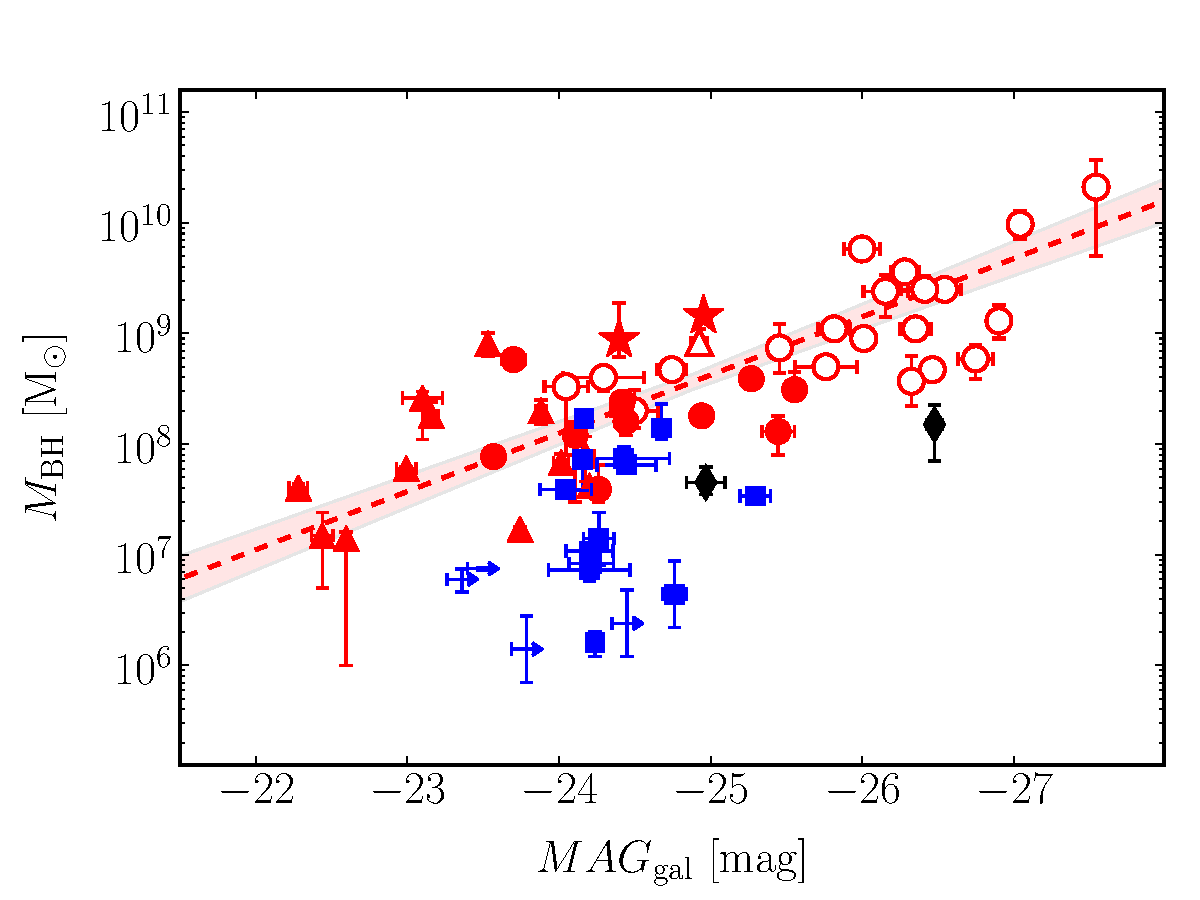
\includegraphics[width=\columnwidth]{images/mbh_vs_mag_tot.pdf}
\caption{Black hole mass plotted against $3.6\rm~\mu m$ galaxy absolute magnitude. 
Symbols are coded according to the galaxy morphological type: red circle = E, red star = E/S0, 
red upward triangle = S0, blue downward triangle = S0/Sp, blue square = Sp, black diamond = merger. 
Empty symbols represent core-S\'ersic spheroids, whereas filled symbols are used for S\'ersic spheroids. 
Four spiral galaxies had their magnitudes overestimated (luminosities underestimated) and are shown as upper limits. 
The red dashed line indicates the BCES bisector linear regression for the 45 early-type galaxies (E+S0), 
with the red shaded area denoting its $1\sigma$ uncertainty. 
$M_{\rm BH}$ correlates equally well with $L_{\rm gal}$ and $L_{\rm sph}$ only for early-type galaxies, 
but not for all (early+late-type) galaxies. }
\label{fig:mbhmaggal}
\end{center}
\end{figure}

\begin{figure}[h]
\begin{center}
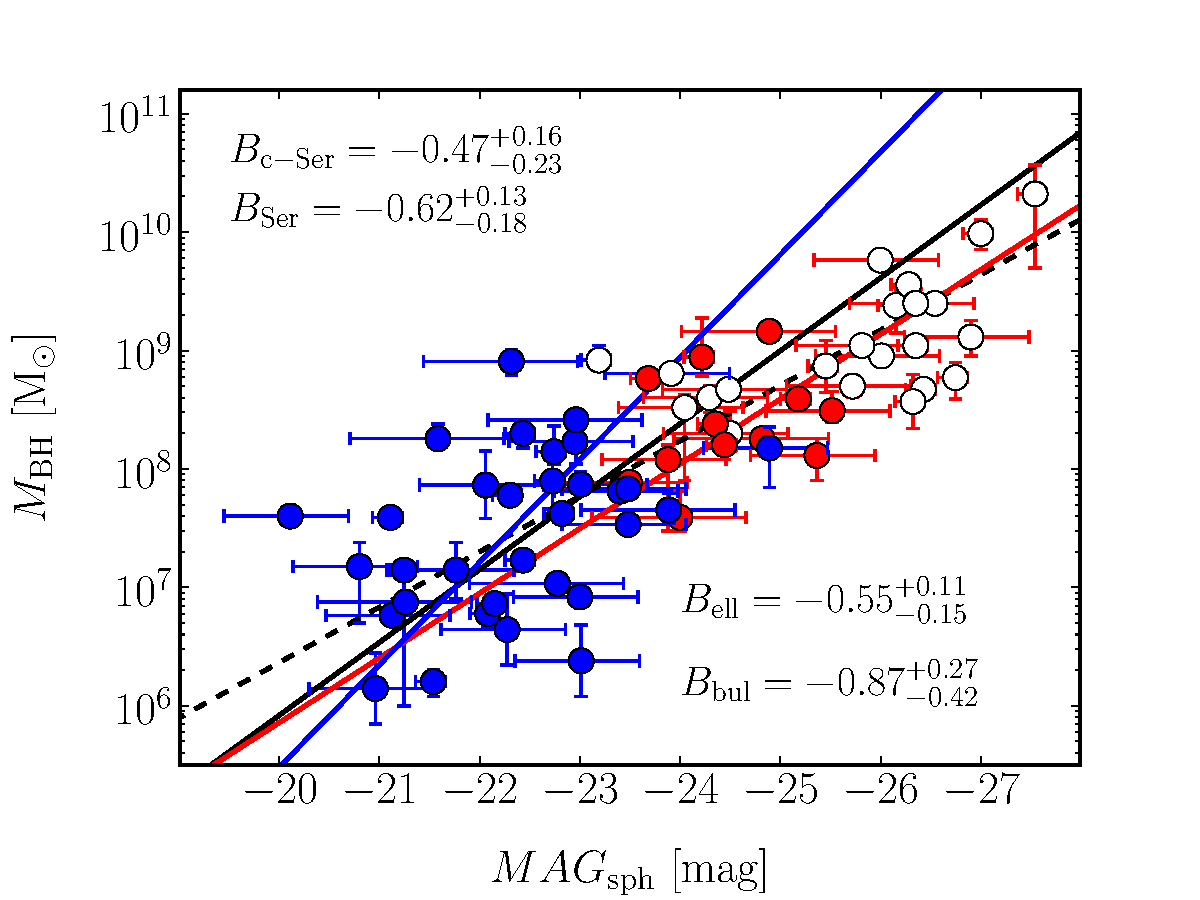
\includegraphics[width=\columnwidth]{images/mbh_vs_mag_sph.pdf}
\caption{Black hole mass plotted against $3.6\rm~\mu m$ spheroid absolute magnitude. 
Symbols have the same meaning as in Figure \ref{fig:mbhmaggal}.
The red dashed line indicates the BCES bisector linear regression for the spheroidal component of the 45 early-type (E+S0) galaxies, 
with the red shaded area denoting its $1\sigma$ uncertainty. 
The blue solid line shows the BCES bisector linear regression for the bulges of the 17 late-type (Sp) galaxies, 
with the blue shaded area denoting its $1\sigma$ uncertainty. 
The black dashed-dotted and dotted lines represent the BCES bisector linear regressions for the core-S\'ersic and S\'ersic spheroids, respectively.}
\label{fig:mbhmagsph}
\end{center}
\end{figure}

\begin{table*}
\centering
\caption{Linear regression analysis of the $M_{\rm BH} - L_{\rm gal}$ diagram.}
\begin{tabular}{llccccc}
\tableline\tableline
{\bf Subsample (size)} & {\bf Regression} & $\boldsymbol \alpha$ & $\boldsymbol \beta$ & $\boldsymbol \langle MAG_{\rm gal} \rangle$ & $\boldsymbol \epsilon$ & $\boldsymbol \Delta$ \\ 
\tableline 
\\
  & \multicolumn{6}{l}{$\log[M_{\rm BH}/{\rm M_\odot}] = \alpha + \beta[(MAG_{\rm gal} - \langle MAG_{\rm gal} \rangle)/{\rm mag}]$} \\ [0.5em]
 All (62)               & BCES $(Y|X)$   & $8.26 \pm 0.08$ & $-0.49 \pm 0.06$ & $-24.78$ & $-$ & $0.64$ \\
                        & mFITEXY $(Y|X)$  & $8.26^{+0.08}_{-0.08}$ & $-0.49^{+0.06}_{-0.07}$ & $-24.78$ & $0.61^{+0.07}_{-0.06}$ & $0.64$ \\
                        & {\tt linmix\_err} $(Y|X)$  & $8.26 \pm 0.09$ & $-0.49 \pm 0.07$ & $-24.78$ & $0.63 \pm 0.07$ & $0.64$ \\ [0.5em]
                        & BCES $(X|Y)$   & $8.26 \pm 0.12$ & $-1.01 \pm 0.15$ & $-24.78$ & $-$ & $0.92$ \\
                        & mFITEXY $(X|Y)$  & $8.26^{+0.11}_{-0.12}$ & $-1.03^{+0.13}_{-0.16}$ & $-24.78$ & $0.88^{+0.10}_{-0.08}$ & $0.93$ \\
                        & {\tt linmix\_err} $(X|Y)$  & $8.26 \pm 0.12$ & $-1.02 \pm 0.15$ & $-24.78$ & $0.91 \pm 0.17$ & $0.93$ \\ [0.5em]
                        & BCES Bisector  & $8.26 \pm 0.09$ & $-0.72 \pm 0.07$ & $-24.78$ & $-$ & $0.71$ \\
                        & mFITEXY Bisector & $8.26^{+0.10}_{-0.10}$ & $-0.73^{+0.09}_{-0.10}$ & $-24.78$ & $-$    & $0.71$ \\
                        & {\tt linmix\_err} Bisector & $8.26 \pm 0.10$ & $-0.72 \pm 0.15$ & $-24.78$ & $-$    & $0.71$ \\ [0.5em]

 Early-type (E+S0) (45) & BCES $(Y|X)$   & $8.56 \pm 0.07$ & $-0.44 \pm 0.05$ & $-24.88$ & $-$ & $0.45$ \\
                        & mFITEXY $(Y|X)$  & $8.56^{+0.06}_{-0.06}$ & $-0.42^{+0.05}_{-0.05}$ & $-24.88$ & $0.41^{+0.06}_{-0.05}$ & $0.45$ \\
                        & {\tt linmix\_err} $(Y|X)$  & $8.56 \pm 0.07$ & $-0.42 \pm 0.06$ & $-24.88$ & $0.43 \pm 0.06$ & $0.45$ \\ [0.5em]
                        & BCES $(X|Y)$   & $8.56 \pm 0.08$ & $-0.64 \pm 0.05$ & $-24.88$ & $-$ & $0.53$ \\
                        & mFITEXY $(X|Y)$  & $8.56^{+0.08}_{-0.08}$ & $-0.66^{+0.07}_{-0.08}$ & $-24.88$ & $0.51^{+0.07}_{-0.06}$ & $0.55$ \\
                        & {\tt linmix\_err} $(X|Y)$  & $8.56 \pm 0.09$ & $-0.65 \pm 0.08$ & $-24.88$ & $0.53 \pm 0.10$ & $0.54$ \\ [0.5em]
                        & BCES Bisector  & $8.56 \pm 0.07$ & $-0.53 \pm 0.04$ & $-24.88$ & $-$ & $0.47$ \\
                        & mFITEXY Bisector & $8.56^{+0.07}_{-0.07}$ & $-0.54^{+0.06}_{-0.06}$ & $-24.88$ & $-$    & $0.47$ \\
                        & {\tt linmix\_err} Bisector & $8.56 \pm 0.08$ & $-0.53 \pm 0.10$ & $-24.88$ & $-$    & $0.47$ \\ [0.5em]

%Late-type (Sp) (13) & BCES $(Y|X)$      & $7.37 \pm 0.17$ & $-0.33 \pm 0.87$   & $-24.39$ & $-$ & $0.65$ \\
%                    & BCES $(X|Y)$      & $7.37 \pm 1.97$ & $-21.66 \pm 53.74$ & $-24.39$ & $-$ & $7.73$ \\
%                    & BCES Bisector     & $7.37 \pm 0.20$ & $-1.32 \pm 0.94$   & $-24.39$ & $-$ & $0.77$ \\
%                    & FITEXY $(Y|X)$    & $7.38^{+0.17}_{-0.18}$ & $-0.34^{+0.74}_{-0.80}$ & $-24.39$ & $0.63^{+0.19}_{-0.11}$ & $0.65$ \\
%                    & FITEXY $(X|Y)$    & $$ & $$ & $-24.39$ & $$ & $$ \\
%                    & FITEXY Bisector   & $$ & $$ & $-24.39$ & $-$    & $$ \\
%                    & {\tt linmix\_err} $(Y|X)$     & $$ & $$ & $-24.39$ & $$ & $$ \\
%                    & {\tt linmix\_err} $(X|Y)$     & $$ & $$ & $-24.39$ & $$ & $$ \\
%                    & {\tt linmix\_err} Bisector    & $$ & $$ & $-24.39$ & $-$    & $$ \\

%All (62)               & BCES $(Y|X)$   & $$ & $$ & $$ & $-$ & $$ \\
%                       & BCES $(X|Y)$   & $$ & $$ & $$ & $-$ & $$ \\
%                       & BCES Bisector     & $$ & $$ & $$ & $-$ & $$ \\
%                       & FITEXY $(Y|X)$ & $$ & $$ & $$ & $$ & $$ \\
%                       & FITEXY $(X|Y)$ & $$ & $$ & $$ & $$ & $$ \\
%                       & FITEXY Bisector   & $$ & $$ & $$ & $-$    & $$ \\
%                       & {\tt linmix\_err} $(Y|X)$  & $$ & $$ & $$ & $$ & $$ \\
%                       & {\tt linmix\_err} $(X|Y)$  & $$ & $$ & $$ & $$ & $$ \\
%                       & {\tt linmix\_err} Bisector    & $$ & $$ & $$ & $-$    & $$ \\

\tableline 
\tableline
\end{tabular}
\label{tab:lreggal} 
\tablecomments{For each subsample, we indicate $\langle MAG_{\rm gal} \rangle$, its average value of galaxy magnitudes. 
In the last two columns, we report $\epsilon$, the intrinsic scatter, and $\Delta$, the total rms scatter in the $\log(M_{\rm BH})$ direction. 
Four spiral galaxies had their luminosities underestimated and thus are not included in the linear regression analysis 
(the sample of all galaxies contains 66-4=62 objects). 
When considering all galaxies, irrespective of their morphological type, 
the $M_{\rm BH} - L_{\rm gal}$ correlation is weaker than the $M_{\rm BH} - L_{\rm sph}$ correlation, in terms of intrinsic scatter. 
However, when considering only early-type galaxies, the $M_{\rm BH} - L_{\rm gal}$ and $M_{\rm BH} - L_{\rm sph}$ correlations 
have consistent intrinsic scatter. }
\end{table*}

\subsection{Black hole mass -- spheroid luminosity}
The $M_{\rm BH} - L_{\rm sph}$ diagram is shown in Figure \ref{fig:mbhmagsph}, 
and the linear regression analysis is presented in Table \ref{tab:lregsph}. 
S\'ersic and core-S\'ersic spheroids have slopes consistent with each other (within their $1\sigma$ uncertainties), 
in disagreement with the findings of GS13. 
The slope that we obtained for core-S\'ersic spheroids ($M_{\rm BH} \propto L_{\rm sph}^{1.18 \pm 0.20}$) 
is consistent with the slope reported by GS13 in the $K_s$-band for the same population ($M_{\rm BH} \propto L_{\rm sph}^{1.10 \pm 0.20}$). 
However, the slope that we determined for S\'ersic spheroids ($M_{\rm BH} \propto L_{\rm sph}^{1.53 \pm 0.20}$) 
is notably shallower than that found by GS13 ($M_{\rm BH} \propto L_{\rm sph}^{2.73 \pm 0.55}$). \\
Although the S\'ersic/core-S\'ersic classification used by GS13 slightly differs\footnote{The classification has changed for the galaxies 
NGC 1316, NGC 1332 and NGC 3998.} from the classification used here, 
the main cause of the inconsistency is that the bulge-to-total ratios obtained from our galaxy decompositions 
are different from those assumed by GS13 to convert galaxy luminosities into bulge luminosities.
Our bulge-to-total ratios for low-luminosity S\'ersic spheroids ($3.6\rm~\mu m$ $MAG_{\rm sph} \gtrsim -22 \rm~mag$) 
are smaller than those used by GS13. 
The host galaxies of such bulges are late-type, spiral galaxies, 
which typically present a complex morphology (bars, double bars, embedded disks, nuclear components, etc).
Our galaxy models account for the extra components, 
while the average bulge-to-total ratios of GS13 were based on less sophisticated S\'ersic-bulge/exponential-disk decompositions 
which overestimated the bulge luminosity.
This results in our bulge magnitudes being on average $\sim$$0.7\rm~mag$ fainter than in GS13, after accounting for the different wavelength of the data.
At the same time, our bulge-to-total ratios for the high-luminosity S\'ersic spheroids ($3.6\rm~\mu m$ $MAG_{\rm sph} \lesssim -24 \rm~mag$) 
are on average larger than those adopted by GS13.
In this regime, the host systems are early-type galaxies that feature intermediate-scale disks\footnote{Intermediate-scale disks are 
disks of stars fully embedded in the spheroidal component of their galaxy. 
They are typical of ``disky'' elliptical galaxies (e.g.~NGC 3377), 
but they can also be found in other types of host galaxies.
They can be considered an intermediate class between nuclear disks, with sizes $\sim$$10-100\rm~pc$, %%
and large-scale disks, that encase the bulge and dominate the light at large radii.}. 
Past bulge/disk decompositions failed to correctly identify the extent of such disks and treated them as large-scale disks, 
thus underestimating the bulge luminosity.
The magnitudes that we obtained for such spheroids are on average $\sim$$0.5\rm~mag$ brighter than in GS13. 
These two effects explain the shallower slope that we obtained for the S\'ersic spheroids. \\
The slope that we obtained for S\'ersic spheroids ($1.53 \pm 0.20$) is not consistent with the value of $2.5$ 
expected from $M_{\rm BH} \propto \sigma^5$ and $L_{\rm sph} \propto \sigma^2$. 
In addition, the S\'ersic and core-S\'ersic spheroids appear not to define two distinct $M_{\rm BH} - L_{\rm sph}$ sequences. 
This leads us to investigate substructure in the $M_{\rm BH} - L_{\rm sph}$ diagram for early- and late-type galaxies.
First, we checked that the elliptical and lenticular galaxies, taken separately, have slopes consistent with each other, 
and thus, taken together, they define a single \emph{early-type sequence} in the $M_{\rm BH} - L_{\rm sph}$ diagram. 
We then fit the early-type galaxies with a single log-linear regression, 
and obtained $M_{\rm BH} \propto L_{\rm sph}^{1.00 \pm 0.10}$. 
We did not find any convincing evidence for the change in slope required for consistency 
with the $M_{\rm BH} - \sigma$ and bent $L_{\rm sph} - \sigma$ correlations. 
Because the change in slope should occur at $M_{\rm BH} > 10^{8 \pm 1}\rm~M_\odot$, 
but all the early-type galaxies in our sample have $M_{\rm BH} \gtrsim 10^7\rm~M_\odot$, 
one possible explanation is that we are still not probing enough low black hole masses for this subsample.
An additional possibility is that there is no sharp transition going from $L_{\rm sph} \propto \sigma^2$ at low luminosities 
to $L_{\rm sph} \propto \sigma^5$ at high luminosities. 
Although the knowledge that many ``elliptical'' galaxies actually contain embedded stellar disks dates back  
at least three decades  
\citep{capaccioli1987,carter1987,rixwhite1990,bender1990,scorzabender1990,nieto1991,rixwhite1992,scorzabender1995},
it is mainly thanks to large integral-field-spectrograph surveys of early-type galaxies, such as the ATLAS$^{\rm 3D}$ Project \citep{cappellari2011}, 
that our view has been further advanced 
and it is now commonly accepted that most ``elliptical'' galaxies contain disks. 
%More than half of all morphologically classified elliptical galaxies in the ATLAS$^{\rm 3D}$ sample are fast rotators \citep{atlas3dIII-MNRAS,krajnovic2013}.
%\cite{krajnovic2013} showed that ``fast rotators'' as a class are disk-galaxies or at least disk-like galaxies. 
%In their magnitude-limited survey, systems 
%without any signature of disk-like components (neither in the kinematics nor in the photometry) 
%dominate only the most massive end (beyond $10^{11.5}~\rm M_\odot$) of the distribution. 
Past studies that investigated the $L_{\rm sph} - \sigma$ diagram might have failed to identify and consequently model the disks 
in intermediate-luminosity, early-type galaxies, thus overestimating $L_{\rm sph}$ 
and mistakenly producing a sharp bend in the $L_{\rm sph} - \sigma$ correlation, rather than a continuously curved relation 
(with $L_{\rm sph} \propto \sigma^{3-4}$ at intermediate luminosities). \\
For the bulges of late-type galaxies we obtained $M_{\rm BH} \propto L_{\rm sph}^{2.88 \pm 0.68}$. 
From a cursory inspection of Figure \ref{fig:mbhmagsph}, one might be tempted to doubt the statistical significance of this ``tentative'' \emph{late-type sequence}. 
However, a visual inspection of the plotted data requires one to take into account the error bars 
when judging-by-eye the strength of a correlation. 
Similarly, the Pearson's and Spearman's correlation coefficients are not applicable because 
they do not take into account the error bars on our data.
We have therefore relied on the quantitative regression analysis.

\subsubsection{Pseudo- versus classical bulges}
Current views distinguish between classical bulges (which are considered to be spheroidal, pressure-supported systems, 
formed through violent processes, such as hierarchical clustering via minor mergers), 
and pseudo-bulges (thought to be disk-like, rotation-supported systems, 
built from secular evolution processes, such as instabilities of their surrounding disk or bar). 
Pseudo-bulges are notoriously hard to identify \citep{graham2013review,graham2014review,graham2015pseudo,graham2015review}.
For example, mergers can create bulges that rotate (e.g.~\citealt{bekki2010,keselmannusser2012}), 
and bars can spin-up classical bulges (e.g.~\citealt{saha2012}), 
thus rotation is not a definitive signature of a pseudo-bulge. 
Furthermore, many galaxies host both a classical and a pseudo-bulge (e.g.~\citealt{erwin2003,erwin2015,athanassoula2005,Gadotti2009,
macarthur2009,dosanjosdasilva2013,seidel2015}). 
In the recent literature, pseudo- and classical bulges have frequently been divided at the 
S\'ersic index $n_{\rm sph}=2$ (e.g.~\citealt{sani2011,beifiori2012}), 
although, from a selection of hundreds of disc galaxies imaged in the $K$-band, 
\cite{grahamworley2008} observed no bimodality in the bulge S\'ersic indices about $n_{\rm sph}=2$ or any other value. 
While pseudo-bulges are expected to have exponential-like surface brightness profiles ($n_{\rm sph} \simeq 1$), 
being disky components that formed from their surrounding exponential disks 
(e.g.~\citealt{bardeen1975,hohl1975,combessanders1981,combes1990,pfennigerfriedli1991}), 
it has been shown that mergers can create bulges with $n_{\rm sph}<2$
(e.g.~\citealt{elichemoral2011,scannapieco2011,querejeta2015}), 
just as low-luminosity elliptical galaxies (not built from the secular evolution of a disk)
are also well known to have $n_{\rm sph}<2$ and even $n_{\rm sph}<1$ (e.g.~\citealt{davies1988,youngcurrie1994,jerjen2000}). 
The use of the S\'ersic index (in addition to rotation) to identify pseudo-bulges is thus a dangerous practice. \\
\cite{sani2011} reported that pseudo-bulges -- which they labelled as such according to the $n_{\rm sph}<2$ criterion -- 
with low black hole masses ($M_{\rm BH} < 10^7\rm~M_\odot$) are significantly displaced from the correlation 
traced by their (classical) bulges with $n_{\rm sph}>2$. 
In Figure \ref{fig:pseudob}, we show the distribution of spheroid S\'ersic indices\footnote{The spheroid S\'ersic indices 
are taken from our galaxy decompositions (\emph{Paper I}).} 
in the $M_{\rm BH} - L_{\rm sph}$ diagram.
Our aim is to check whether bulges with $n_{\rm sph}<2$ 
are offset to lower black hole masses from the correlation defined by bulges with $n_{\rm sph}>2$. 
To do this, we fit a symmetrical linear regression to the bulges that have $n_{\rm sph}>2$ 
and we then compute the vertical offset of all bulges from this regression. 
In Figure \ref{fig:pseudob}, we plot the vertical offset against $n_{\rm sph}$. 
Among the 23 bulges with $n_{\rm sph}<2$, 12 have a positive vertical offset and 11 have a negative vertical offset. 
\cite{kormendy2015review} provides a list of many pseudo-bulge classification criteria, including the divide at $n_{\rm sph}=2$, 
and cautions that each individual criterion has a failure rate of 0-25\%. 
If this is true, we should have that no less than 75\% of bulges with $n_{\rm sph}<2$ display a negative vertical offset\footnote{One 
reaches the same conclusion when using the vertical offset from the correlation defined by bulges with $n_{\rm sph}>3$ or even $n_{\rm sph}>4$. 
There are 13 and 10 bulges with $n_{\rm sph}<2$ that lie above and below, respectively, the correlation traced by bulges with $n_{\rm sph}>3$. 
Similarly, there are 15 and 8 bulges with $n_{\rm sph}<2$ that lie above and below, respectively, the correlation traced by bulges with $n_{\rm sph}>4$.}. 
What we observe, instead, is that there are the same number of bulges with $n_{\rm sph}<2$ lying above and below 
the correlation defined by bulges with $n_{\rm sph}>2$, 
and that the amplitude of their offset is the same ($\lesssim 1.5\rm~dex$).
That is, bulges with $n_{\rm sph}<2$ do not appear to be offset from the correlation traced by bulges with $n_{\rm sph}>2$. 


\begin{figure}[h]
\begin{center}
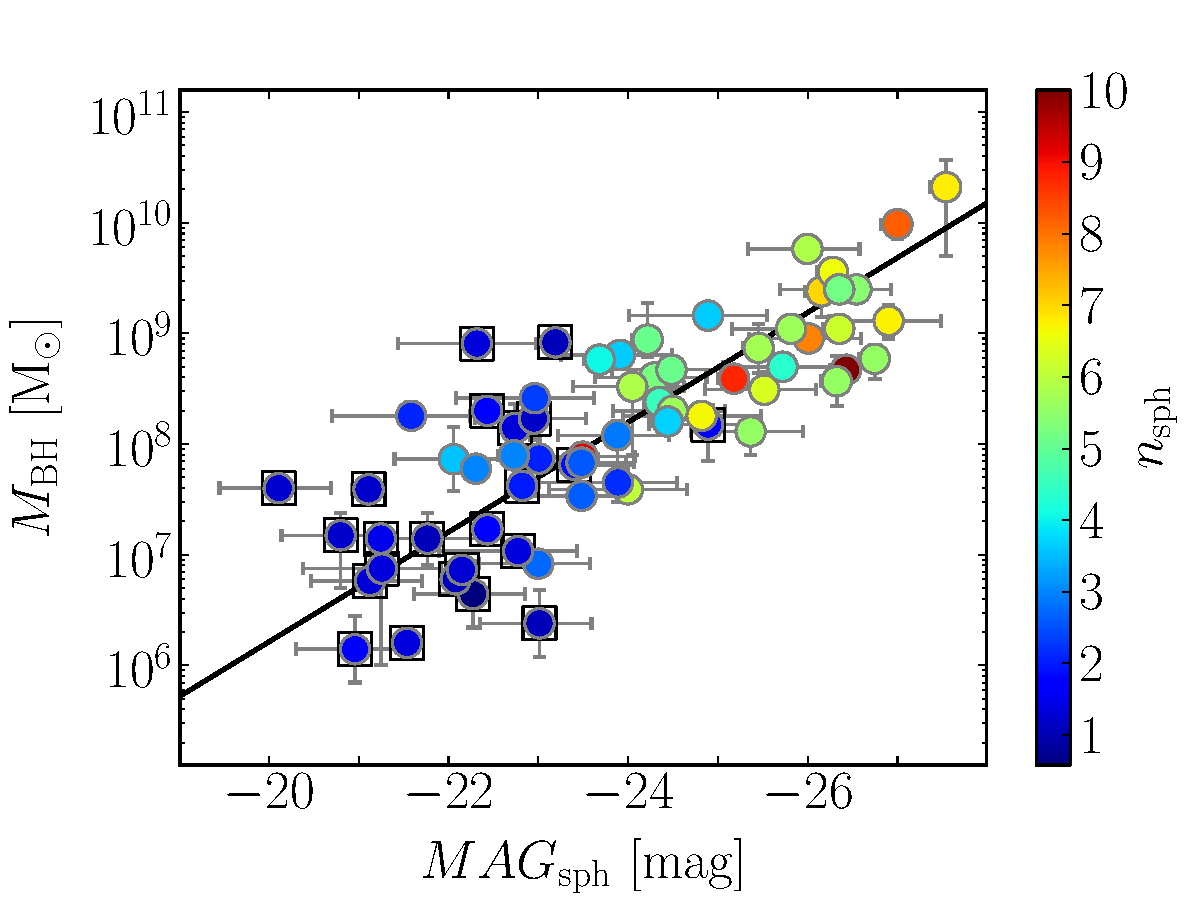
\includegraphics[width=\columnwidth]{images/mbh_vs_mag_sph_psb.pdf}
\caption{Black hole mass plotted against $3.6\rm~\mu m$ spheroid absolute magnitude (as in Figure \ref{fig:mbhmagsph}). 
Symbols are color coded according to the spheroid S\'ersic index $n_{\rm sph}$. 
Bulges with $n_{\rm sph}<2$, claimed by some to be pseudo-bulges, are enclosed with a square. 
The black solid line shows the BCES bisector linear regression for the spheroids that have $n_{\rm sph} \geq 2$, 
such that $M_{\rm BH} \propto L_{\rm sph}^{1.25 \pm 0.13}$. }
\label{fig:pseudob}
\end{center}
\end{figure}


\begin{figure}[h]
\begin{center}
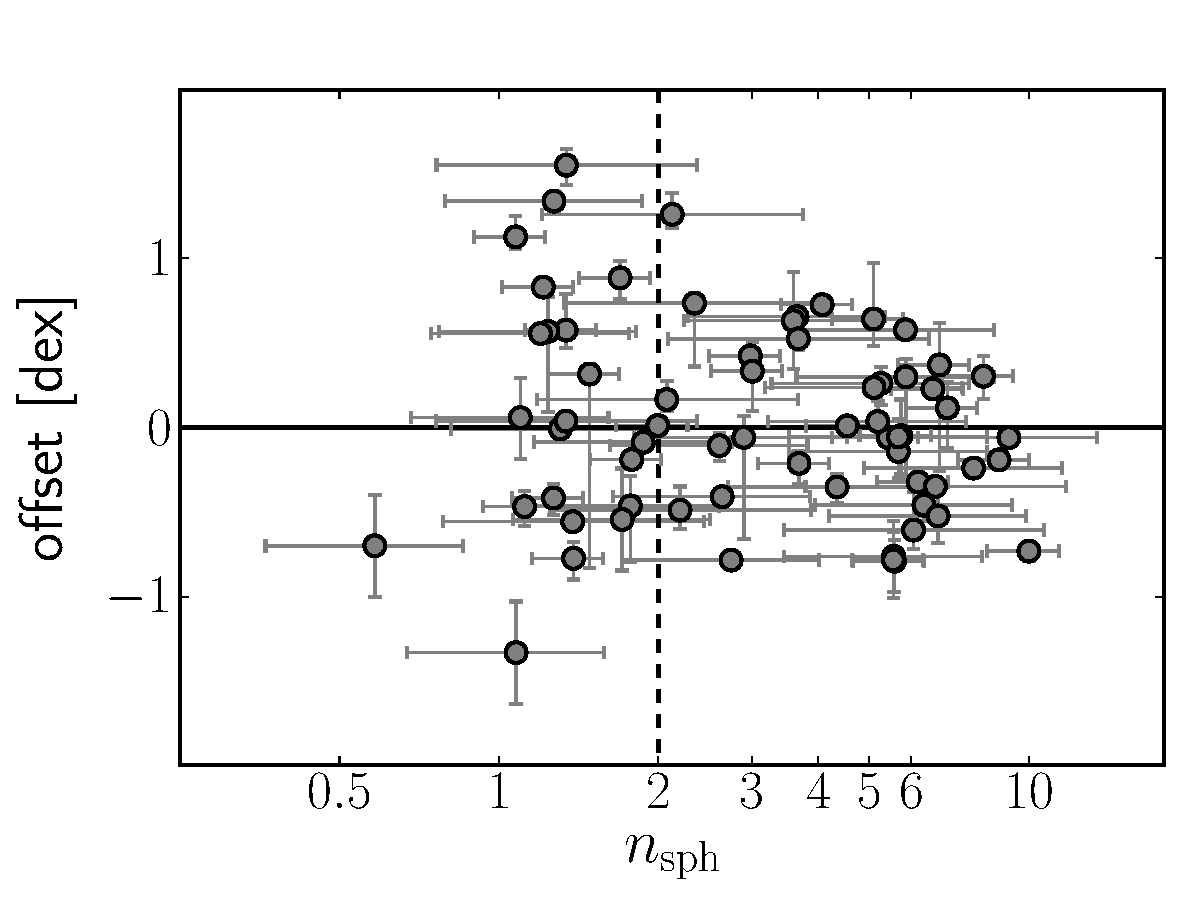
\includegraphics[width=\columnwidth]{images/inset_psb.pdf}
\caption{Vertical offset from the $M_{\rm BH} - L_{\rm sph}$ correlation defined by spheroids with $n_{\rm sph} \geq 2$ (see Figure \ref{fig:pseudob}), 
plotted against $n_{\rm sph}$. 
The vertical dashed line corresponds to $n_{\rm sph} = 2$.
The horizontal solid line is equivalent to a zero vertical offset.
Among the bulges with $n_{\rm sph}<2$, 12 have a positive vertical offset and 11 have a negative vertical offset.
Hence, bulges with $n_{\rm sph}<2$ are not randomly offset to lower black hole masses 
from the correlation traced by bulges with $n_{\rm sph} \geq 2$.}
\label{fig:offset}
\end{center}
\end{figure}


\begin{table*}
\centering
\caption{Linear regression analysis of the $M_{\rm BH} - L_{\rm sph}$ diagram.}
\begin{tabular}{llccccc}
\tableline
\tableline
{\bf Subsample (size)} & {\bf Regression} & $\boldsymbol \alpha$ & $\boldsymbol \beta$ & $\boldsymbol \langle MAG_{\rm sph} \rangle$ & $\boldsymbol \epsilon$ & $\boldsymbol \Delta$ \\ 
\tableline 
\\
 & \multicolumn{6}{l}{$\log[M_{\rm BH}/{\rm M_\odot}] = \alpha + \beta[(MAG_{\rm sph} - \langle MAG_{\rm sph} \rangle)/{\rm mag}]$} \\ [0.5em]
All (66)               & BCES $(Y|X)$   & $8.16 \pm 0.07$ & $-0.44 \pm 0.04$ & $-23.86$ & $-$ & $0.56$ \\
                       & mFITEXY $(Y|X)$    & $8.17^{+0.06}_{-0.07}$ & $-0.43^{+0.03}_{-0.04}$ & $-23.86$ & $0.49^{+0.06}_{-0.05}$ & $0.56$ \\
                       & {\tt linmix\_err} $(Y|X)$     & $8.16 \pm 0.07$ & $-0.42 \pm 0.04$ & $-23.86$ & $0.51 \pm 0.06$ & $0.56$ \\ [0.5em]
                       & BCES $(X|Y)$   & $8.16 \pm 0.08$ & $-0.61 \pm 0.05$ & $-23.86$ & $-$ & $0.68$ \\
                       & mFITEXY $(X|Y)$    & $8.15^{+0.07}_{-0.08}$ & $-0.61^{+0.05}_{-0.05}$ & $-23.86$ & $0.58^{+0.07}_{-0.06}$ & $0.68$ \\
                       & {\tt linmix\_err} $(X|Y)$     & $8.16 \pm 0.09$ & $-0.60 \pm 0.06$ & $-23.86$ & $0.60 \pm 0.09$ & $0.67$ \\ [0.5em]
                       & BCES Bisector  & $8.16 \pm 0.07$ & $-0.52 \pm 0.04$ & $-23.86$ & $-$ & $0.60$ \\
                       & mFITEXY Bisector   & $8.16^{+0.07}_{-0.07}$ & $-0.51^{+0.04}_{-0.04}$ & $-23.86$ & $-$    & $0.60$ \\
                       & {\tt linmix\_err} Bisector    & $8.16 \pm 0.08$ & $-0.51 \pm 0.09$ & $-23.86$ & $-$    & $0.59$ \\ [0.5em]

$n>2$ (43)             & BCES $(Y|X)$      & $8.58 \pm 0.07$ & $-0.42 \pm 0.06$ & $-24.77$ & $-$ & $0.46$ \\
                       & mFITEXY $(Y|X)$    & $8.57^{+0.07}_{-0.06}$ & $-0.41^{+0.04}_{-0.04}$ & $-24.77$ & $0.38^{+0.06}_{-0.06}$ & $0.46$ \\
                       & {\tt linmix\_err} $(Y|X)$     & $8.56 \pm 0.07$ & $-0.39 \pm 0.05$ & $-24.77$ & $0.40 \pm 0.06$ & $0.46$ \\ [0.5em]
                       & BCES $(X|Y)$      & $8.58 \pm 0.08$ & $-0.58 \pm 0.06$ & $-24.77$ & $-$ & $0.56$ \\
                       & mFITEXY $(X|Y)$    & $8.56^{+0.08}_{-0.08}$ & $-0.57^{+0.06}_{-0.07}$ & $-24.77$ & $0.44^{+0.08}_{-0.11}$ & $0.55$ \\
                       & {\tt linmix\_err} $(X|Y)$     & $8.55 \pm 0.09$ & $-0.57 \pm 0.08$ & $-24.77$ & $0.49 \pm 0.10$ & $0.55$ \\ [0.5em]
                       & BCES Bisector     & $8.58 \pm 0.07$ & $-0.50 \pm 0.05$ & $-24.77$ & $-$ & $0.49$ \\
                       & mFITEXY Bisector   & $8.57^{+0.07}_{-0.07}$ & $-0.49^{+0.05}_{-0.05}$ & $-24.77$ & $-$    & $0.49$ \\
                       & {\tt linmix\_err} Bisector    & $8.56 \pm 0.08$ & $-0.48 \pm 0.10$ & $-24.77$ & $-$    & $0.49$ \\  [0.5em]
                   
Core-S\'ersic (22) & BCES $(Y|X)$   & $9.06 \pm 0.09$ & $-0.32 \pm 0.11$  & $-25.73$ & $-$    & $0.42$ \\
                   & mFITEXY $(Y|X)$   & $9.06^{+0.08}_{-0.09}$ & $-0.26^{+0.08}_{-0.07}$ & $-25.73$ & $0.36^{+0.09}_{-0.06}$ & $0.42$ \\
                   & {\tt linmix\_err} $(Y|X)$  & $9.04 \pm 0.10$ & $-0.24 \pm 0.09$ & $-25.73$ & $0.40 \pm 0.08$ & $0.42$ \\ [0.5em]
                   & BCES $(X|Y)$   & $9.06 \pm 0.12$ & $-0.65 \pm 0.12$  & $-25.73$ & $-$    & $0.61$ \\
                   & mFITEXY $(X|Y)$   & $9.03^{+0.15}_{-0.16}$ & $-0.72^{+0.17}_{-0.31}$ & $-25.73$ & $0.61^{+0.14}_{-0.09}$ & $0.68$ \\
                   & {\tt linmix\_err} $(X|Y)$  & $9.03 \pm 0.17$ & $-0.69 \pm 0.27$ & $-25.73$ & $0.68 \pm 0.30$ & $0.64$ \\ [0.5em]
                   & BCES Bisector  & $9.06 \pm 0.10$ & $-0.47 \pm 0.08$  & $-25.73$ & $-$    & $0.48$ \\
                   & mFITEXY Bisector  & $9.05^{+0.12}_{-0.13}$ & $-0.47^{+0.12}_{-0.17}$ & $-25.73$ & $-$    & $0.48$ \\
                   & {\tt linmix\_err} Bisector & $9.04 \pm 0.14$ & $-0.44 \pm 0.16$ & $-25.73$ & $-$    & $0.46$ \\ [0.5em]

S\'ersic (44) & BCES $(Y|X)$   & $7.71 \pm 0.09$ & $-0.41 \pm 0.08$ & $-22.92$ & $-$    & $0.61$ \\
              & mFITEXY $(Y|X)$   & $7.72^{+0.08}_{-0.09}$ & $-0.41^{+0.07}_{-0.08}$ & $-22.92$ & $0.54^{+0.08}_{-0.07}$ & $0.61$ \\
              & {\tt linmix\_err} $(Y|X)$  & $7.73 \pm 0.09$ & $-0.41 \pm 0.08$ & $-22.92$ & $0.55 \pm 0.08$ & $0.61$ \\ [0.5em]
              & BCES $(X|Y)$   & $7.71 \pm 0.14$ & $-0.86 \pm 0.16$ & $-22.92$ & $-$    & $0.93$ \\
              & mFITEXY $(X|Y)$   & $7.72^{+0.14}_{-0.13}$ & $-0.86^{+0.13}_{-0.19}$ & $-22.92$ & $0.77^{+0.13}_{-0.10}$ & $0.93$ \\
              & {\tt linmix\_err} $(X|Y)$  & $7.73 \pm 0.14$ & $-0.86 \pm 0.17$ & $-22.92$ & $0.79 \pm  0.20$ & $0.93$ \\ [0.5em]
              & BCES Bisector  & $7.71 \pm 0.10$  & $-0.61 \pm 0.08$ & $-22.92$ & $-$    & $0.71$ \\
              & mFITEXY Bisector  & $7.72^{+0.11}_{-0.11}$ & $-0.61^{+0.10}_{-0.12}$ & $-22.92$ & $-$                    & $0.71$ \\
              & {\tt linmix\_err} Bisector & $7.73 \pm 0.12$ & $-0.62 \pm 0.15$ & $-22.92$ & $-$    & $0.71$ \\ [0.5em]

%Ellipticals (E) (30)   & BCES $(Y|X)$   & $8.80 \pm 0.07$ & $-0.53 \pm 0.09$ & $-25.45$ & $-$    & $0.42$ \\
%                      & BCES $(X|Y)$   & $8.80 \pm 0.08$ & $-0.66 \pm 0.07$ & $-25.45$ & $-$    & $0.48$ \\
%                      & BCES Bisector     & $8.80 \pm 0.08$ & $-0.59 \pm 0.07$ & $-25.45$ & $-$    & $0.44$ \\
%                      & FITEXY $(Y|X)$ & $8.81^{+0.07}_{-0.07}$ & $-0.44^{+0.06}_{-0.07}$ & $-25.45$ & $0.33$     & $0.40$ \\
%                      & FITEXY $(X|Y)$ & $8.78^{+0.09}_{-0.09}$ & $-0.7^{+0.1}_{-0.1}$    & $-25.45$ & $0.60$     & $0.50$\\
%                      & FITEXY Bisector   & $8.80^{+0.08}_{-0.08}$ & $-0.56^{+0.08}_{-0.10}$ & $-25.45$ & $-$        & $0.43$ \\
%
%Lenticulars (S0) (13)  & BCES $(Y|X)$   & $7.9 \pm 0.1$ & $-0.4 \pm 0.2$ & $-22.19$ & $-$    & $0.56$ \\
%                      & BCES $(X|Y)$   & $7.9 \pm 0.3$ & $-1.1 \pm 0.5$ & $-22.19$ & $-$    & $1.01$ \\
%                      & BCES Bisector     & $7.9 \pm 0.2$ & $-0.7 \pm 0.2$ & $-22.19$ & $-$    & $0.69$ \\
%                      & FITEXY $(Y|X)$ & $7.9^{+0.2}_{-0.1}$ & $-0.3^{+0.2}_{-0.2}$ & $-22.19$ & $0.51$     & $0.56$ \\
%                      & FITEXY $(X|Y)$ & $7.8^{+0.3}_{-0.4}$ & $-1.3^{+0.4}_{-1.3}$ & $-22.19$ & $0.71$     & $1.20$\\
%                      & FITEXY Bisector   & $7.9^{+0.2}_{-0.3}$ & $-0.7^{+0.3}_{-0.4}$ & $-22.19$ & $-$        & $0.71$ \\
%

{\bf Early-type (E+S0)} (45) & BCES $(Y|X)$    & $8.56 \pm 0.07$ & $-0.33 \pm 0.04$ & $-24.47$ & $-$    & $0.46$ \\
                             & mFITEXY $(Y|X)$ & $8.56^{+0.06}_{-0.06}$ & $-0.32^{+0.03}_{-0.04}$ & $-24.47$ & $0.40^{+0.06}_{-0.05}$ & $0.46$ \\
                             & {\tt linmix\_err} $(Y|X)$  & $8.55 \pm 0.07$ & $-0.32 \pm 0.04$ & $-24.47$ & $0.41 \pm 0.06$ & $0.46$ \\ [0.5em]
                             & BCES $(X|Y)$    & $8.56 \pm 0.08$ & $-0.48 \pm 0.05$ & $-24.47$ & $-$    & $0.55$ \\
                             & mFITEXY $(X|Y)$ & $8.54^{+0.08}_{-0.08}$ & $-0.49^{+0.05}_{-0.06}$ & $-24.47$ & $0.49^{+0.08}_{-0.06}$ & $0.57$\\
                             & {\tt linmix\_err} $(X|Y)$  & $8.55 \pm 0.09$ & $-0.48 \pm 0.06$ & $-24.47$ & $0.51 \pm 0.10$ & $0.56$ \\ [0.5em]
                             & {\bf BCES Bisector}& $\boldsymbol{8.56 \pm 0.07}$ & $\boldsymbol{-0.40 \pm 0.04}$ & $\boldsymbol{-24.47}$ & $-$    & $\boldsymbol{0.49}$ \\
                             & mFITEXY Bisector   & $8.55^{+0.07}_{-0.07}$ & $-0.41^{+0.04}_{-0.05}$ & $-24.47$ & $-$    & $0.49$ \\
                             & {\tt linmix\_err} Bisector    & $8.55 \pm 0.08$ & $-0.40 \pm 0.09$ & $-24.47$ & $-$    & $0.49$ \\ [0.5em]

{\bf Late-type (Sp)} (17) & BCES $(Y|X)$    & $7.18 \pm 0.16$ & $-0.79 \pm 0.43$ & $-22.33$ & $-$    & $0.70$ \\
                          & mFITEXY $(Y|X)$    & $7.20^{+0.15}_{-0.15}$ & $-0.53^{+0.22}_{-0.24}$ & $-22.33$ & $0.55^{+0.15}_{-0.10}$ & $0.63$ \\
                          & {\tt linmix\_err} $(Y|X)$  & $7.24 \pm 0.19$ & $-0.46 \pm 0.32$ & $-22.33$ & $0.63 \pm 0.16$ & $0.62$ \\ [0.5em]
                          & BCES $(X|Y)$    & $7.18 \pm 0.29$ & $-1.71 \pm 0.71$ & $-22.33$ & $-$    & $1.26$ \\
                          & mFITEXY $(X|Y)$    & $7.38^{+0.54}_{-0.36}$ & $-2.02^{+0.71}_{-2.13}$ & $-22.33$ & $1.09^{+0.41}_{-0.24}$ & $1.50$ \\
                          & {\tt linmix\_err} $(X|Y)$  & $7.34 \pm 0.43$ & $-1.93 \pm 1.30$ & $-22.33$ & $1.31 \pm 0.97$ & $1.43$ \\ [0.5em]
                          & {\bf BCES Bisector}& $\boldsymbol{7.18 \pm 0.20}$ & $\boldsymbol{-1.15 \pm 0.27}$ & $\boldsymbol{-22.33}$ & $-$    & $\boldsymbol{0.88}$ \\
                          & mFITEXY Bisector   & $7.26^{+0.40}_{-0.28}$ & $-1.03^{+0.33}_{-0.52}$ & $-22.33$ & $-$    & $0.82$ \\
                          & {\tt linmix\_err} Bisector & $7.27 \pm 0.33$ & $-0.96 \pm 0.50$ & $-22.33$ & $-$    & $0.78$ \\ [0.5em]

\tableline 
\tableline
\end{tabular}
\label{tab:lregsph} 
\tablecomments{For each subsample, we indicate $\langle MAG_{\rm sph} \rangle$, its average value of spheroid magnitudes. 
In the last two columns, we report $\epsilon$, the intrinsic scatter, and $\Delta$, the total rms scatter in the $\log(M_{\rm BH})$ direction. 
Both the early- and late-type subsamples do not contain the two galaxies classified as S0/Sp and the two galaxies classified as mergers (45+17=66-2-2). }
\end{table*}


\subsection{Black hole mass -- spheroid stellar mass}
Finally, we present the $M_{\rm BH} - M_{\rm *,sph}$ diagram in Figure \ref{fig:mbhmasssph}, 
and its linear regression analysis in Table \ref{tab:lregmass}. 
The bulges of the early-type galaxies follow $M_{\rm BH} \propto M_{\rm *,sph}^{1.04 \pm 0.10}$,
consistent with a dry-merging formation scenario,
and define a tight \emph{early-type sequence} with intrinsic scatter $\epsilon_{(Y|X)} = 0.43 \pm 0.06\rm~dex$. 
\cite{graham2012bent} reported that the $M_{\rm BH}/M_{\rm dyn,sph}$ ratio for core-S\'ersic galaxies was 0.36\% 
($M_{\rm dyn,sph}$ is the spheroid dynamical mass), 
and discussed the many implications of this.  
Using a larger data sample, \cite{grahamscott2013} reported that the $M_{\rm BH}/M_{\rm *,sph}$ ratio was 0.49\% for core-S\'ersic galaxies.   
Here we find a median $M_{\rm BH}/M_{\rm *,sph}$ ratio of $0.50 \pm 0.04\%$ for the 22 core-S\'ersic galaxies 
and $0.68 \pm 0.04\%$ for the 45 early-type galaxies.  
Among other things, this higher value (previously reported to be $0.1 - 0.2\%$ for all galaxy types, e.g.~\citealt{marconihunt2003}), 
boosts estimates of the black hole mass function and mass density based on galaxy/spheroid luminosity functions. \\
The bulges of the spiral galaxies trace a steeper \emph{late-type sequence}, 
whose slope is less well constrained due to the smaller size of the subsample and, more importantly, 
to the smaller range in $M_{\rm *,sph}$ that the subsample spans. 
For the bulges of spiral galaxies, the BCES code returns a log-linear relation with a slope $= 3.00 \pm 1.30$, 
while the modified FITEXY routine finds a shallower (but still consistent within the $1\sigma$ uncertainty) 
slope $= 2.28^{+1.67}_{-1.01}$.
%The Bayesian estimator of \cite{linmixerr} fails in performing an inverse $(X|Y)$ linear regression for the subsample of spiral galaxies. 
More data would be welcome to better constrain the slope of this \emph{late-type sequence}, 
although we note that direct measurements of black hole masses below $10^6\rm~M_\odot$ are extremely challenging to obtain 
with the current technological resources. 
In this regard, using a sample of $\sim$140 low-redshift ($z \leq 0.35$, with a median redshift $\langle z \rangle = 0.085$) 
bulges hosting Active Galactic Nuclei (AGNs) with virial
black hole masses $10^5 \lesssim M_{\rm BH}/{\rm M_\odot} \lesssim 2 \times 10^6$ \citep{jiang2011a}, 
\cite{grahamscott2015} showed that they roughly follow the quadratic $M_{\rm BH} - M_{\rm *,sph}$ relation defined by their S\'ersic bulges.
The majority of our spiral galaxies host an AGN\footnote{According to the nuclear classification reported on NED 
(NASA Extragalactic Database), among our 17 spiral galaxies, at least 12 host a Seyfert AGN and one hosts a LINER AGN.} and
we anticipate here that the correlation traced by our spiral galaxy bulges 
may track the location of these lower mass AGN in the $M_{\rm BH} - M_{\rm *,sph}$ diagram.
That is, the AGNs appear to be the low-mass continuation of our tentative \emph{late-type sequence} shown in Figure \ref{fig:mbhmasssph} 
and this will be explored with more rigour in a forthcoming paper. 
 

\begin{figure}[h]
\begin{center}
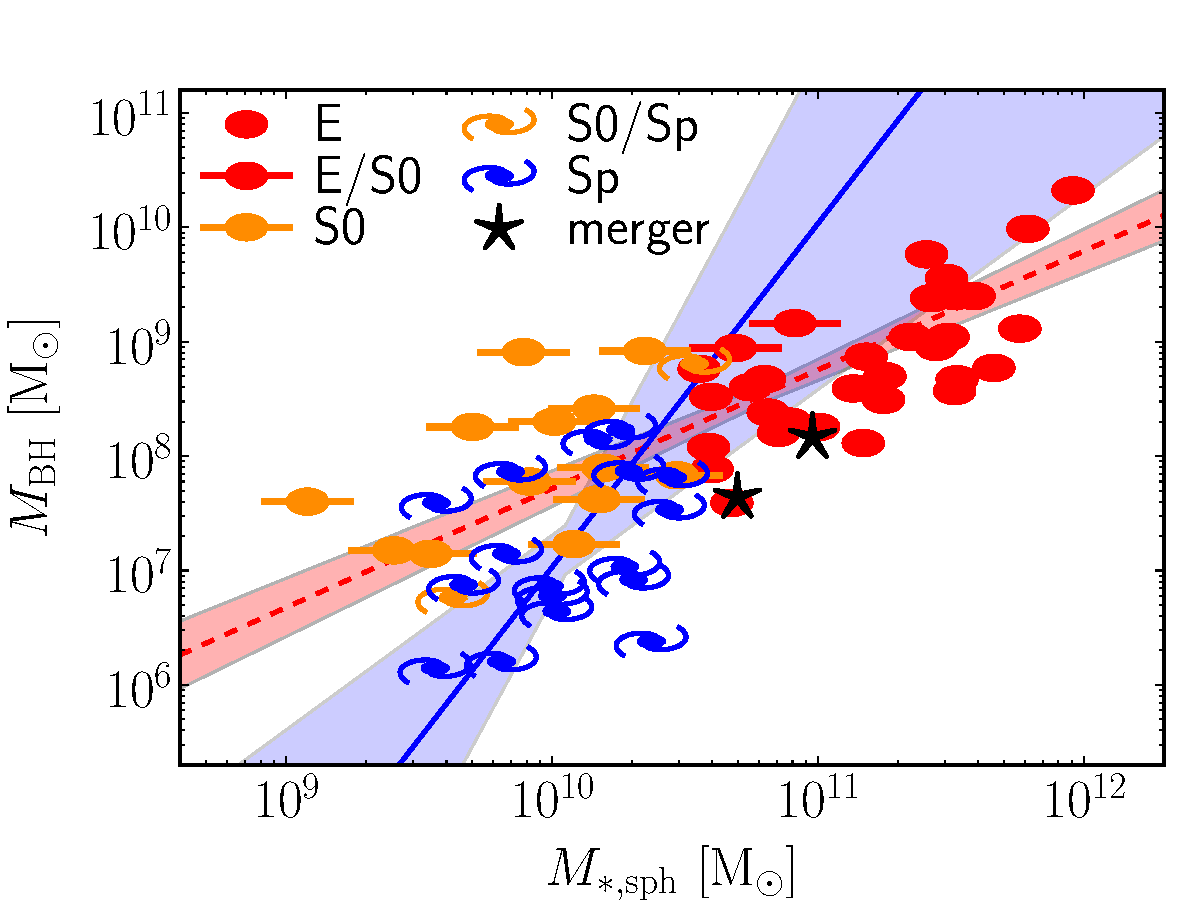
\includegraphics[width=\columnwidth]{images/mbh_vs_mass_sph.pdf}
\caption{Black hole mass plotted against spheroid stellar mass. 
Symbols are coded according to the galaxy morphological type (see legend).
The red dashed line indicates the BCES bisector linear regression for the bulges of the 45 early-type galaxies (E+S0), 
with the red shaded area denoting its $1\sigma$ uncertainty. 
The bulges of early-type galaxies follow $M_{\rm BH} \propto M_{\rm *,sph}^{1.04 \pm 0.10}$,
a near-linear relation consistent with a dry-merging formation scenario.
The steeper blue solid line shows the BCES bisector linear regression for the bulges of the 17 late-type (Sp) galaxies, 
with the blue shaded area denoting its $1\sigma$ uncertainty. 
The bulges of late-type galaxies follow $M_{\rm BH} \propto M_{\rm *,sph}^{2-3}$, 
indicating that gas-rich processes feed the black hole more efficiently (``quadratically'' or ``cubically'') than the host bulge grows in stellar mass. 
We note that AGNs with $10^5 \lesssim M_{\rm BH}/{\rm M_\odot} \lesssim 2 \times 10^6$ \citep{jiang2011a} appear to follow the blue line 
(see Graham et al. 2015, \emph{in preparation}).}
\label{fig:mbhmasssph}
\end{center}
\end{figure}

\section{Conclusions}
Using $3.6\rm~\mu m$ \emph{Spitzer} images, 
we have performed accurate multicomponent decompositions (i.e.~bulge, disks, bars, spiral arms, rings, halo, nucleus, depleted core, etc.), 
which were checked to be consistent with the two-dimensional galaxy kinematics, 
for 66 nearby galaxies with a dynamical measurement of their black hole mass.
We have derived galaxy luminosities, spheroid luminosities and spheroid stellar masses. 
Our galaxy sample, besides being to date the largest sample with reliable bulge masses used to investigate black hole mass scaling relations, 
contains 17 spiral galaxies, half of which have $M_{\rm BH} < 10^7 \rm~M_{\odot}$. 
This constitutes a significant improvement over past studies whose samples were biased towards high-mass, early-type galaxies. \\
Using our state-of-the-art dataset, we have investigated substructure in the $M_{\rm BH} - L_{\rm gal}$, $M_{\rm BH} - L_{\rm sph}$ 
and $M_{\rm BH} - M_{\rm *,sph}$ diagrams. 
Our principal conclusions are: \\

\begin{itemize}
\item The logarithmic $M_{\rm BH} - M_{\rm *,sph}$ relation for the spheroidal components of early-type (elliptical + lenticular) galaxies 
      has a slope of $1.04 \pm 0.10$ and intrinsic scatter $\epsilon_{(Y|X)} = 0.43 \pm 0.06\rm~dex$. 
      We call this tight correlation an \emph{early-type sequence}. 
      The $M_{\rm BH} - M_{\rm *,sph}$ log-relation for the bulges of late-type (spiral) galaxies has a slope of $2-3$,
      which is less well constrained due to
      the smaller size of the subsample and, more importantly, the smaller range in spheroid stellar mass 
      ($3 \times 10^9 \lesssim M_{\rm *,sph}/{\rm M_\odot} \lesssim 3 \times 10^{10}$) that the subsample spans. 
      We refer to this correlation as a \emph{late-type sequence}. 
      In (gas-poor) early-type galaxies, the black hole and the stellar content of the spheroidal component grow at the same pace, 
      following a linear $M_{\rm BH} - M_{\rm *,sph}$ relation. 
      In (gas-rich) spiral galaxies, the black hole grows faster than its host bulge, 
      following a quadratic/cubic $M_{\rm BH} - M_{\rm *,sph}$ relation. 
      Unsurprisingly, in a color-magnitude diagram\footnote{Total $B-V$ colors, 
      corrected for inclination, Galactic extinction and K-correction, 
      were taken from the HyperLEDA online database \citep{hyperleda}.}, 
      our early- and late-type galaxies occupy the two distinct regions of the red sequence and the blue cloud, respectively. 
      For analogy with this, we refer to our \emph{early-type sequence} as a \emph{red sequence} 
      and to our \emph{late-type sequence} as a \emph{blue sequence}. 
      %For analogy with the color-magnitude diagram, 
      %it may be tempting to refer to our \emph{early-type sequence} as a \emph{red sequence} 
      %and to our \emph{late-type sequence} as a \emph{blue sequence}.
      %Future work will explore the color of spheroids and galaxies in the $M_{\rm BH} - M_{\rm *,sph}$ diagram.  
\item The median $M_{\rm BH}/M_{\rm *,sph}$ ratio for the early-type galaxies is $0.68 \pm 0.04\%$. 
      This value is dramatically larger than what was previously reported ($0.1 - 0.2\%$ for all galaxy types, e.g.~\citealt{marconihunt2003}), 
      but in close agreement with the value of $0.49\%$ reported by \cite{grahamscott2013} for core-S\'ersic spheroids. 
\item The logarithmic $M_{\rm BH} - M_{\rm *,sph}$ relations for the core-S\'ersic and S\'ersic spheroids 
      have slopes with over-lapping uncertainties ($1.19 \pm 0.23$ and $1.48 \pm 0.20$, respectively).  
      The S\'ersic relation is less steep than, but also has over-lapping uncertainties with, 
      the slope of $2.22 \pm 0.58$ reported by \cite{scott2013} for S\'ersic spheroids.  
      The distinction between core-S\'ersic and S\'ersic spheroids found by \cite{scott2013} is thus less pronounced here. 
\item In the $M_{\rm BH} - L_{\rm sph}$ (or $M_{\rm BH} - M_{\rm *,sph}$) diagram, for early-type galaxies, 
      we did not observe the change in slope required for consistency with the log-linear $M_{\rm BH} - \sigma$ and bent $L_{\rm sph} - \sigma$ correlations.
      This issue of inconsistency remains therefore an open question. 
      It might be that we are still not probing enough low-mass black holes ($M_{\rm BH} < 10^7\rm~M_\odot$) 
      for the subsample of early-type galaxies, 
      or that the transition from  $L_{\rm sph} \propto \sigma^2$ at low luminosities to $L_{\rm sph} \propto \sigma^{(5-6)}$ at high luminosities 
      is less sharp than previously thought.
      We intend to investigate this point in our future work. 
\item Spheroids with S\'ersic index $n_{\rm sph}<2$, argued by some to be pseudo-bulges, 
      are not offset to lower $M_{\rm BH}$ from the $M_{\rm BH} - L_{\rm sph}$ correlation defined by spheroids with $n_{\rm sph}>2$. 
\item The $M_{\rm BH} - L_{\rm gal}$ and $M_{\rm BH} - L_{\rm sph}$ correlations have the same level of intrinsic scatter 
      when considering early-type galaxies only. 
      Once reasonable numbers of spiral galaxies are included, 
      $M_{\rm BH}$ correlates better with $L_{\rm sph}$ than with $L_{\rm gal}$. 
\end{itemize} 

Finally, we note that some of the literature-sourced black hole mass measurements used by \cite{kormendyho2013} are different from those used here.  
While these differences are smaller than $18\%$ for $78\%$ of the galaxies, 
in three cases (NGC 0821, NGC 4291, and NGC 3393) they are larger than a factor of $2.3$.  
We repeated our entire analysis using only the 58 galaxies that are in common between our sample and the sample of \cite{kormendyho2013}, 
assuming for these galaxies the black hole mass measurements published by \cite{kormendyho2013}. 
In doing so, we found that none of our conclusions changed.


\begin{table*}
\centering
\caption{Linear regression analysis of the $M_{\rm BH} - M_{\rm *,sph}$ diagram.}
\begin{tabular}{llccccc}
\tableline
\tableline
{\bf Subsample (size)} & {\bf Regression} & $\boldsymbol \alpha$ & $\boldsymbol \beta$ & $\boldsymbol \langle M_{\rm *,sph} \rangle$ & $\boldsymbol \epsilon$ & $\boldsymbol \Delta$ \\ 
\tableline 
\\
  & \multicolumn{6}{l}{$\log[M_{\rm BH}/{\rm M_\odot}] = \alpha + \beta \log[(M_{\rm *,sph} / \langle M_{\rm *,sph} \rangle)]$} \\ [0.5em]
 Core-S\'ersic (22)     & BCES $(Y|X)$      & $9.06 \pm 0.09$ & $0.86 \pm 0.28$ & $10^{11.28}$ & $-$ & $0.42$ \\
 			& mFITEXY $(Y|X)$   & $9.06^{+0.08}_{-0.08}$ & $0.68^{+0.21}_{-0.20}$ & $10^{11.28}$ & $0.36^{+0.09}_{-0.06}$ & $0.42$ \\
  			& {\tt linmix\_err} $(Y|X)$     & $9.04 \pm 0.10$ & $0.64 \pm 0.25$ & $10^{11.28}$ & $0.40 \pm 0.09$ & $0.42$ \\ [0.5em]
			& BCES $(X|Y)$      & $9.06 \pm 0.12$ & $1.70 \pm 0.32$ & $10^{11.28}$ & $-$ & $0.61$ \\
 			& mFITEXY $(X|Y)$   & $9.03^{+0.15}_{-0.16}$ & $1.90^{+0.85}_{-0.46}$ & $10^{11.28}$ & $0.62^{+0.13}_{-0.10}$ & $0.68$ \\
 			& {\tt linmix\_err} $(X|Y)$     & $9.03 \pm 0.17$ & $1.80 \pm 0.70$ & $10^{11.28}$ & $0.67 \pm 0.30$ & $0.65$ \\ [0.5em]
 			& BCES Bisector     & $9.06 \pm 0.10$ & $1.19 \pm 0.23$ & $10^{11.28}$ & $-$ & $0.47$ \\
 			& mFITEXY Bisector  & $9.05^{+0.12}_{-0.13}$ & $1.12^{+0.35}_{-0.27}$ & $10^{11.28}$ & $-$                    & $0.46$ \\
 			& {\tt linmix\_err} Bisector	& $9.04 \pm 0.14$ & $1.06 \pm 0.35$ & $10^{11.28}$ & $-$	& $0.45$ \\ [0.5em]

 S\'ersic (44)		& BCES $(Y|X)$      & $7.71 \pm 0.09$ & $0.95 \pm 0.21$ & $10^{10.25}$ & $-$ & $0.64$ \\
 			& mFITEXY $(Y|X)$   & $7.72^{+0.10}_{-0.09}$ & $0.96^{+0.21}_{-0.21}$ & $10^{10.25}$ & $0.58^{+0.09}_{-0.07}$ & $0.64$ \\
 			& {\tt linmix\_err} $(Y|X)$     & $7.73 \pm 0.10$ & $0.98 \pm 0.24$ & $10^{10.25}$ & $0.59 \pm 0.08$ & $0.65$ \\ [0.5em]
 			& BCES $(X|Y)$      & $7.71 \pm 0.16$ & $2.52 \pm 0.54$ & $10^{10.25}$ & $-$ & $1.11$ \\
 			& mFITEXY $(X|Y)$   & $7.72^{+0.16}_{-0.16}$ & $2.49^{+0.69}_{-0.45}$ & $10^{10.25}$ & $0.93^{+0.15}_{-0.13}$ & $1.10$ \\
 			& {\tt linmix\_err} $(X|Y)$     & $7.73 \pm 0.17$ & $2.48 \pm 0.59$ & $10^{10.25}$ & $0.95 \pm 0.27$ & $1.10$ \\ [0.5em]
 			& BCES Bisector     & $7.71 \pm 0.11$ & $1.48 \pm 0.20$ & $10^{10.25}$ & $-$ & $0.74$ \\
 			& mFITEXY Bisector  & $7.72^{+0.13}_{-0.13}$ & $1.49^{+0.33}_{-0.28}$ & $10^{10.25}$ & $-$    & $0.74$ \\
 			& {\tt linmix\_err} Bisector	& $7.73 \pm 0.14$ & $1.49 \pm 0.57$ & $10^{10.25}$ & $-$	& $0.74$ \\ [0.5em]

{\bf Early-type (E+S0)} (45)  & BCES $(Y|X)$       & $8.56 \pm 0.07$ & $0.85 \pm 0.12$ & $10^{10.81}$ & $-$ & $0.48$ \\
                              & mFITEXY $(Y|X)$     & $8.56^{+0.06}_{-0.07}$ & $0.83^{+0.11}_{-0.11}$ & $10^{10.81}$ & $0.42^{+0.07}_{-0.05}$ & $0.48$ \\
                              & {\tt linmix\_err} $(Y|X)$     & $8.55 \pm 0.07$ & $0.82 \pm 0.12$ & $10^{10.81}$ & $0.43 \pm 0.06$ & $0.48$ \\ [0.5em]
                              & BCES $(X|Y)$       & $8.56 \pm 0.09$ & $1.27 \pm 0.13$ & $10^{10.81}$ & $-$ & $0.59$ \\
                              & mFITEXY $(X|Y)$     & $8.54^{+0.08}_{-0.09}$ & $1.32^{+0.18}_{-0.15}$ & $10^{10.81}$ & $0.53^{+0.08}_{-0.07}$ & $0.61$ \\
                              & {\tt linmix\_err} $(X|Y)$     & $8.55 \pm 0.09$ & $1.29 \pm 0.17$ & $10^{10.81}$ & $0.54 \pm 0.11$ & $0.59$ \\ [0.5em]
                              & {\bf BCES Bisector}& $\boldsymbol{8.56 \pm 0.07}$ & $\boldsymbol{1.04 \pm 0.10}$ & $\boldsymbol{10^{10.81}}$ & $-$ & $\boldsymbol{0.51}$ \\
                              & mFITEXY Bisector    & $8.55^{+0.07}_{-0.08}$ & $1.05^{+0.14}_{-0.12}$ & $10^{10.81}$ & $-$                    & $0.51$ \\
                              & {\tt linmix\_err} Bisector    & $8.55 \pm 0.08$ & $1.03 \pm 0.19$ & $10^{10.81}$ & $-$    & $0.51$ \\ [0.5em]

{\bf Late-type (Sp)} (17)    & BCES $(Y|X)$    & $7.18 \pm 0.17$ & $1.95 \pm 1.52$ & $10^{10.05}$ & $-$ & $0.74$ \\ 
                             & mFITEXY $(Y|X)$     & $7.20^{+0.15}_{-0.16}$ & $1.22^{+0.70}_{-0.62}$  & $10^{10.05}$ & $0.59^{+0.16}_{-0.11}$ & $0.66$ \\
                             & {\tt linmix\_err} $(Y|X)$  & $7.23 \pm 0.19$ & $0.96 \pm 0.96$ & $10^{10.05}$ & $0.67 \pm 0.16$ & $0.65$ \\ [0.5em]
                             & BCES $(X|Y)$    & $7.18 \pm 0.39$ & $5.89 \pm 3.40$ & $10^{10.05}$ & $-$ & $1.70$ \\
                             & mFITEXY $(X|Y)$     & $7.44^{+1.45}_{-0.52}$ & $7.14^{+26.31}_{-3.01}$ & $10^{10.05}$ & $1.49^{+0.56}_{-0.36}$ & $2.08$ \\
                             & {\tt linmix\_err} $(X|Y)$  & $7.42 \pm 0.64$ & $6.96 \pm 6.73$ & $10^{10.05}$ & $1.83 \pm 1.86$ & $2.03$ \\ [0.5em]
                             & {\bf BCES Bisector}& $\boldsymbol{7.18 \pm 0.21}$ & $\boldsymbol{3.00 \pm 1.30}$ & $\boldsymbol{10^{10.05}}$ & $-$ & $\boldsymbol{0.94}$ \\
                             & {\bf mFITEXY Bisector}    & $\boldsymbol{7.24^{+1.04}_{-0.39}}$ & $\boldsymbol{2.28^{+1.67}_{-1.01}}$  & $\boldsymbol{10^{10.05}}$ & $-$    & $\boldsymbol{0.79}$ \\
                             & {\tt linmix\_err} Bisector & $7.26 \pm 0.47$ & $1.94 \pm 216.38$ & $10^{10.05}$ & $-$    & $0.74$ \\ [0.5em]
                  
\tableline 
\tableline
\end{tabular}
\label{tab:lregmass} 
\tablecomments{For each subsample, we indicate $\langle M_{\rm *,sph} \rangle$, its average value of spheroid stellar masses. 
In the last two columns, we report $\epsilon$, the intrinsic scatter, and $\Delta$, the total rms scatter in the $\log(M_{\rm BH})$ direction. }
\end{table*}


\acknowledgments
GS warmly thanks Luca Cortese, Elisabete Lima Da Cunha, Duncan Forbes and Gonzalo Diaz for useful discussion. \\
% referee thank you!!
This research was supported by Australian Research Council funding through grants
DP110103509 and FT110100263.
This work is based on observations made with the IRAC instrument \citep{fazio2004IRAC} 
on-board the Spitzer Space Telescope, 
which is operated by the Jet Propulsion Laboratory, 
California Institute of Technology under a contract with NASA.
This research has made use of the GOLDMine database \citep{goldmine} and the NASA/IPAC Extragalactic Database (NED) 
which is operated by the Jet Propulsion Laboratory, California Institute of Technology, 
under contract with the National Aeronautics and Space Administration. 
We acknowledge the usage of the HyperLeda database (\url{http://leda.univ-lyon1.fr}).
The BCES routine \citep{akritasbershady1996} was run via the python module 
written by Rodrigo Nemmen \citep{nemmen2012}, which is available at \url{https://github.com/rsnemmen/BCES}.

\bibliography{/Users/gsavorgnan/galaxy_vivisection/papers/SMBHbibliography}


\clearpage


\end{document}



\chapter{$M_{\rm BH} - n_{\rm sph}$}
\label{ch:mn}

While the previous Chapter was dedicated to the study of the relations between 
black hole mass and galaxy or spheroid luminosity, 
in this Chapter we perform an analogous analysis 
to explore the relation between black hole mass and spheroid S\'ersic index ($M_{\rm BH} - n_{\rm sph}$). 
To address the issue of consistency between galaxy scaling relations 
that was outlined in Chapter \ref{ch:intro}, 
it is mandatory to include also an analysis of the relation between spheroid luminosity 
and spheroid S\'ersic index ($L_{\rm sph} - n_{\rm sph}$). 
The reliability of the uncertainties associated with the S\'ersic index measurements 
obtained from our 1D decompositions 
ensures a robust estimate of the intrinsic scatter in the $M_{\rm BH} - n_{\rm sph}$ diagram, 
which can be compared with that in the $M_{\rm BH} - L_{\rm sph}$ diagram. \\ 

From a physical point of view, the $M_{\rm BH} - n_{\rm sph}$ correlation is interesting because 
the S\'ersic index is a measure of the central radial concentration of stars, 
which dictates the radial distribution of mass within a galaxy's spheroid 
and therefore determines the dynamical response of stars 
as measured through the observable $\sigma_*$ \citep{grahamdriver2007}. \\

The remainder of this Chapter comprises the published version of the paper 
``Supermassive Black Holes and Their Host Spheroids. 
III. The $M_{\rm BH} - n_{\rm sph}$ correlation'' 
by G.~A.~D.~Savorgnan,  
as it appears in Volume 821 of the \emph{The Astrophysical Journal}. 



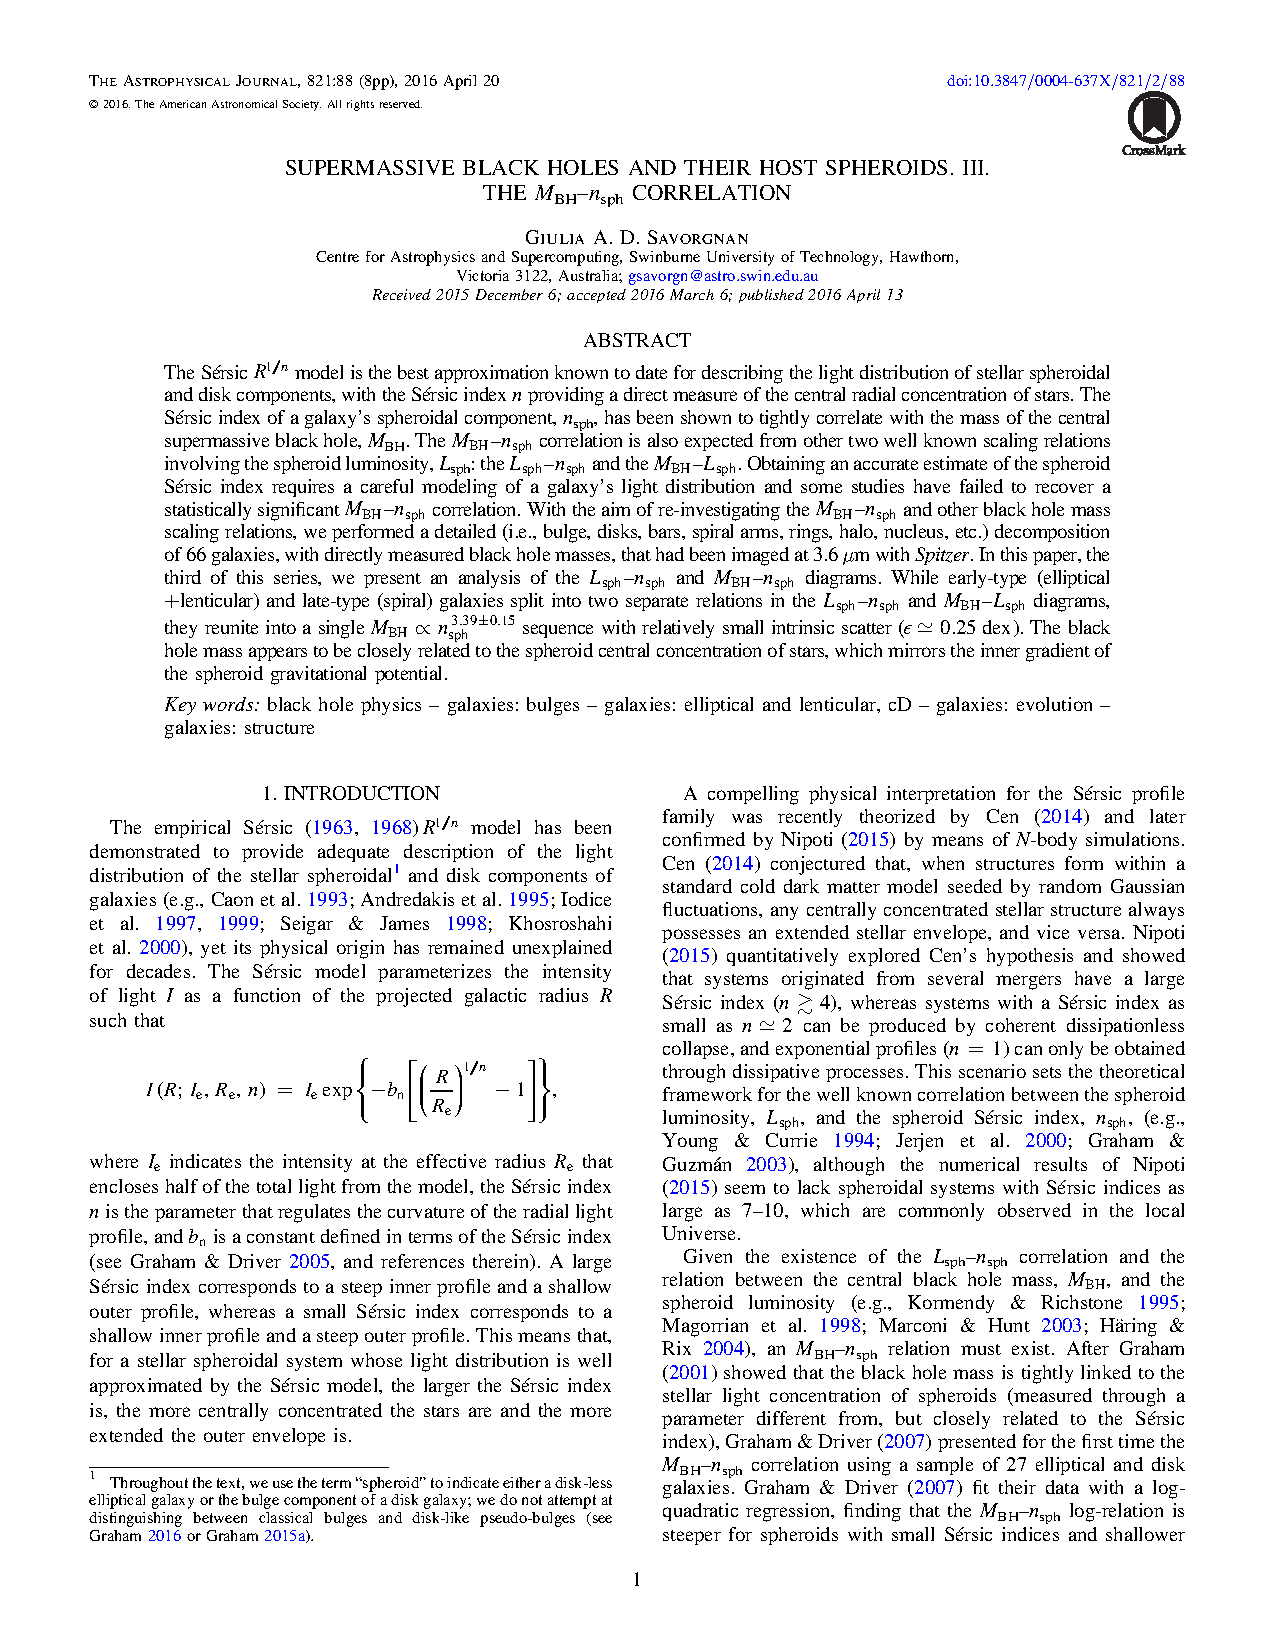
\includepdf[pages={1-8}]{ApJ2016b.pdf}


\chapter{Monster Black Holes in Massive Galaxies}
\label{ch:msigma}

A precise measurement of the log-slope of the $M_{\rm BH} - \sigma_*$ correlation is important 
to constrain theoretical models of AGN feedback. 
For example, energy driven outflows are expected to produce a scaling of $M_{\rm BH} \propto \sigma_*^5$, 
whereas momentum driven outflows should result into a shallower $M_{\rm BH} \propto \sigma_*^4$ relation 
\citep{silkrees1998,fabian1999}. 
Since the $M_{\rm BH} - \sigma_*$ correlation was presented for the first time by \citet{ferraresemerritt2000}
and \citet{gebhardt2000}, 
there has been an ongoing, lively debate about its log-slope, 
whose estimates differed by up to a few standard deviations 
depending on the choice of galaxy sample, the method used to measure the velocity dispersion,
the assumed uncertainty associated with the velocity dispersion, 
and the linear regression algorithm (e.g.~\citealt{tremaine2002}). \\ 

Recent measurements of SMBH masses in Central Cluster Galaxies (CCGs)
have added new data points at the high-mass end of the 
$M_{\rm BH} - \sigma_*$ diagram \citep{mcconnell2011,mcconnell2012}, 
which appear to be outlying (``over-massive'') with respect to the observed correlation. 
\citet{volontericiotti2013} explained the presence of over-massive black holes in CCGs 
(they included in this definition either central dominant galaxies or brightest cluster galaxies) 
as a natural consequence of the fact that these galaxies have experienced more dry mergers 
than any other early-type galaxy (see also \citealt{kormendyho2013}). 
Their semi-analytical models are based on the idea that parabolic dissipationless dry mergers 
increase a galaxy's mass, luminosity and effective radius, 
but do not significantly change its velocity dispersion (e.g.~\citealt{ciotti2007}). 
Let an elliptical galaxy be a non rotating, isotropic and virialized spheroidal system 
with stellar mass $M_{*}$ and gas mass $M_{\rm g} = \alpha M_{*}$. 
The total energy $E$ of this galaxy is the sum of its total kinetic energy $K$ and its total gravitational energy $W$. 
The total kinetic energy is given by the sum of the stellar kinetic energy $K_*$ and the gas internal energy $K_{\rm g}$, 
therefore the total energy can be expressed as:
\begin{equation}
E = K_* + K_{\rm g} + W \ .
\end{equation}
The stellar kinetic energy is 
\begin{equation}
K_* = \frac{3}{2} M_* \sigma_*^2 \ ,
\end{equation}
where $\sigma_*$ is the stellar velocity dispersion. \\
The gas internal energy is defined as 
\begin{equation}
K_{\rm g} = \frac{3}{2} \frac{k_{\rm B}}{\bar{m} } \int_{\mathcal{V}} \rho_{\rm g} T d\mathcal{V} \ ,
\end{equation}
where $k_{\rm B}$ is the Boltzmann constant, $\bar{m}$ is the gas mean molecular mass, and 
$\rho_{\rm g}$ and $T$ are the density spatial distribution and the temperature of the gas, respectively, 
within the galaxy's volume $\mathcal{V}$. \\
The total gravitational energy is defined as 
\begin{equation}
W = \frac{1}{2} \int_{\mathcal{V}} (\rho_* + \rho_{\rm g}) (\phi_* + \phi_{\rm g}) d\mathcal{V} \ , 
\end{equation}
where $\rho_*$ is the density spatial distribution of stars, 
and $\phi_*$ and $\phi_{\rm g}$ indicate the gravitational potential of stars and gas, respectively. \\
Under the assumption of gas in equilibrium in the total gravitational field, 
from the Jeans and hydrostatic equations one has that $T = \bar{m} \sigma_*^2 / k_{\rm B}$ and thus 
\begin{equation}
K_{\rm g} = \alpha K_* \ .
\end{equation}
Assuming also that the spatial distribution of gas is proportional to that of stars (i.e.~$\rho_{\rm g} = \alpha \rho_*$ 
and $\phi_{\rm g} = \alpha \phi_*$), 
the total gravitational energy can be written as 
\begin{equation}
W = \frac{1}{2} (1+\alpha)^2 \int_{\mathcal{V}} \rho_* \phi_* d\mathcal{V} = (1+\alpha)^2 W_* \ ,
\end{equation}
where $W_*$ is the gravitational energy of the stellar component only. \\
From the virial theorem (i.e.~$E = K+W = W/2 = -2K$), the galaxy's total energy can be expressed as 
\begin{equation}
E = \frac{1}{2} (1+\alpha)^2 W_* = - (1+\alpha) K_* \ .
\end{equation}
We now consider the parabolic dissipationless merger of two galaxies (with stellar masses $M_{*1}$ and $M_{*2}$,
and total energies $E_1$ and $E_2$), 
i.e.~a merger where both the total energy and the total mass are conserved, 
and no gas is converted into stars. \\
The gas fraction $\alpha$ of the merger remnant is by definition
\begin{equation}
\alpha = \frac{M_{\rm g}}{M_*} = \frac{M_{\rm g1} + M_{\rm g2}}{M_{*1}+M_{*2}} \ ,
\end{equation}
where the nomenclature is self-explicative. \\
By imposing the conservation of total energy, we get 
\begin{equation*}
E = E_1 + E_2 
\end{equation*}
\begin{equation*}
-(1+\alpha) \frac{3}{2} M_* \sigma_*^2 = -(1+\alpha_1) \frac{3}{2} M_{*1} \sigma_{*1}^2 -(1+\alpha_2) \frac{3}{2} M_{*2} \sigma_{*2}^2 \\
\end{equation*}
\begin{equation*}
\bigl[ (1+\alpha_1)M_{*1} + (1+\alpha_2)M_{*2} \bigr ] \sigma_*^2 = (1+\alpha_1)M_{*1}\sigma_{*1}^2 + (1+\alpha_2)M_{*2}\sigma_{*2}^2
\end{equation*}
\begin{equation}
\sigma_*^2 = \frac{(1+\alpha_1)M_{*1}\sigma_{*1}^2 + (1+\alpha_2)M_{*2}\sigma_{*2}^2}{\bigl[ (1+\alpha_1)M_{*1} + (1+\alpha_2)M_{*2} \bigr ]} \ .
\label{eq:sigma*2}
\end{equation}
By defining $c_1 = (1+\alpha_1)M_{*1}/\bigl[ (1+\alpha_1)M_{*1} + (1+\alpha_2)M_{*2} \bigr ]$ 
and $c_2 = (1+\alpha_2)M_{*2}/\bigl[ (1+\alpha_1)M_{*1} + (1+\alpha_2)M_{*2} \bigr ]$, 
Equation \ref{eq:sigma*2} can be simplified as 
\begin{equation}
\sigma_*^2 = c_1 \sigma_{*1}^2 + c_2 \sigma_{*2}^2 \ .
\end{equation}
Finally, since $c_1 + c_2 = 1$, we have that 
\begin{equation}
\min(\sigma_{*1}^2, \sigma_{*2}^2) \leq \sigma_*^2 \leq \max(\sigma_{*1}^2, \sigma_{*2}^2) \ ,
\end{equation}
that is, the velocity dispersion of the merger remnant cannot be larger 
than the maximum velocity dispersion of the progenitor galaxies. 
This conclusion is not true in case of a wet merger or non-parabolic (i.e.~bound) orbits of the progenitors. \\

Whether or not considering the over-massive black holes as an ``exception to the rule'', 
or in other words legitimately excluding them from the linear regression analysis of the $M_{\rm BH} - \sigma_*$ diagram, 
obviously has an impact on the estimate of the log-slope of the correlation. 
Therefore, it is important to test the scenario proposed by \citet{volontericiotti2013} 
with empirical data. \\

The remainder of this Chapter comprises the published version of the paper 
``Overmassive black holes in the $M_{\rm BH} - \sigma$ diagram 
do not belong to over (dry) merged galaxies'' 
by G.~A.~D.~Savorgnan \& A.~W.~Graham,  
as it appears in Volume 446 of \emph{Monthly Notices of the Royal Astronomical Society}. 


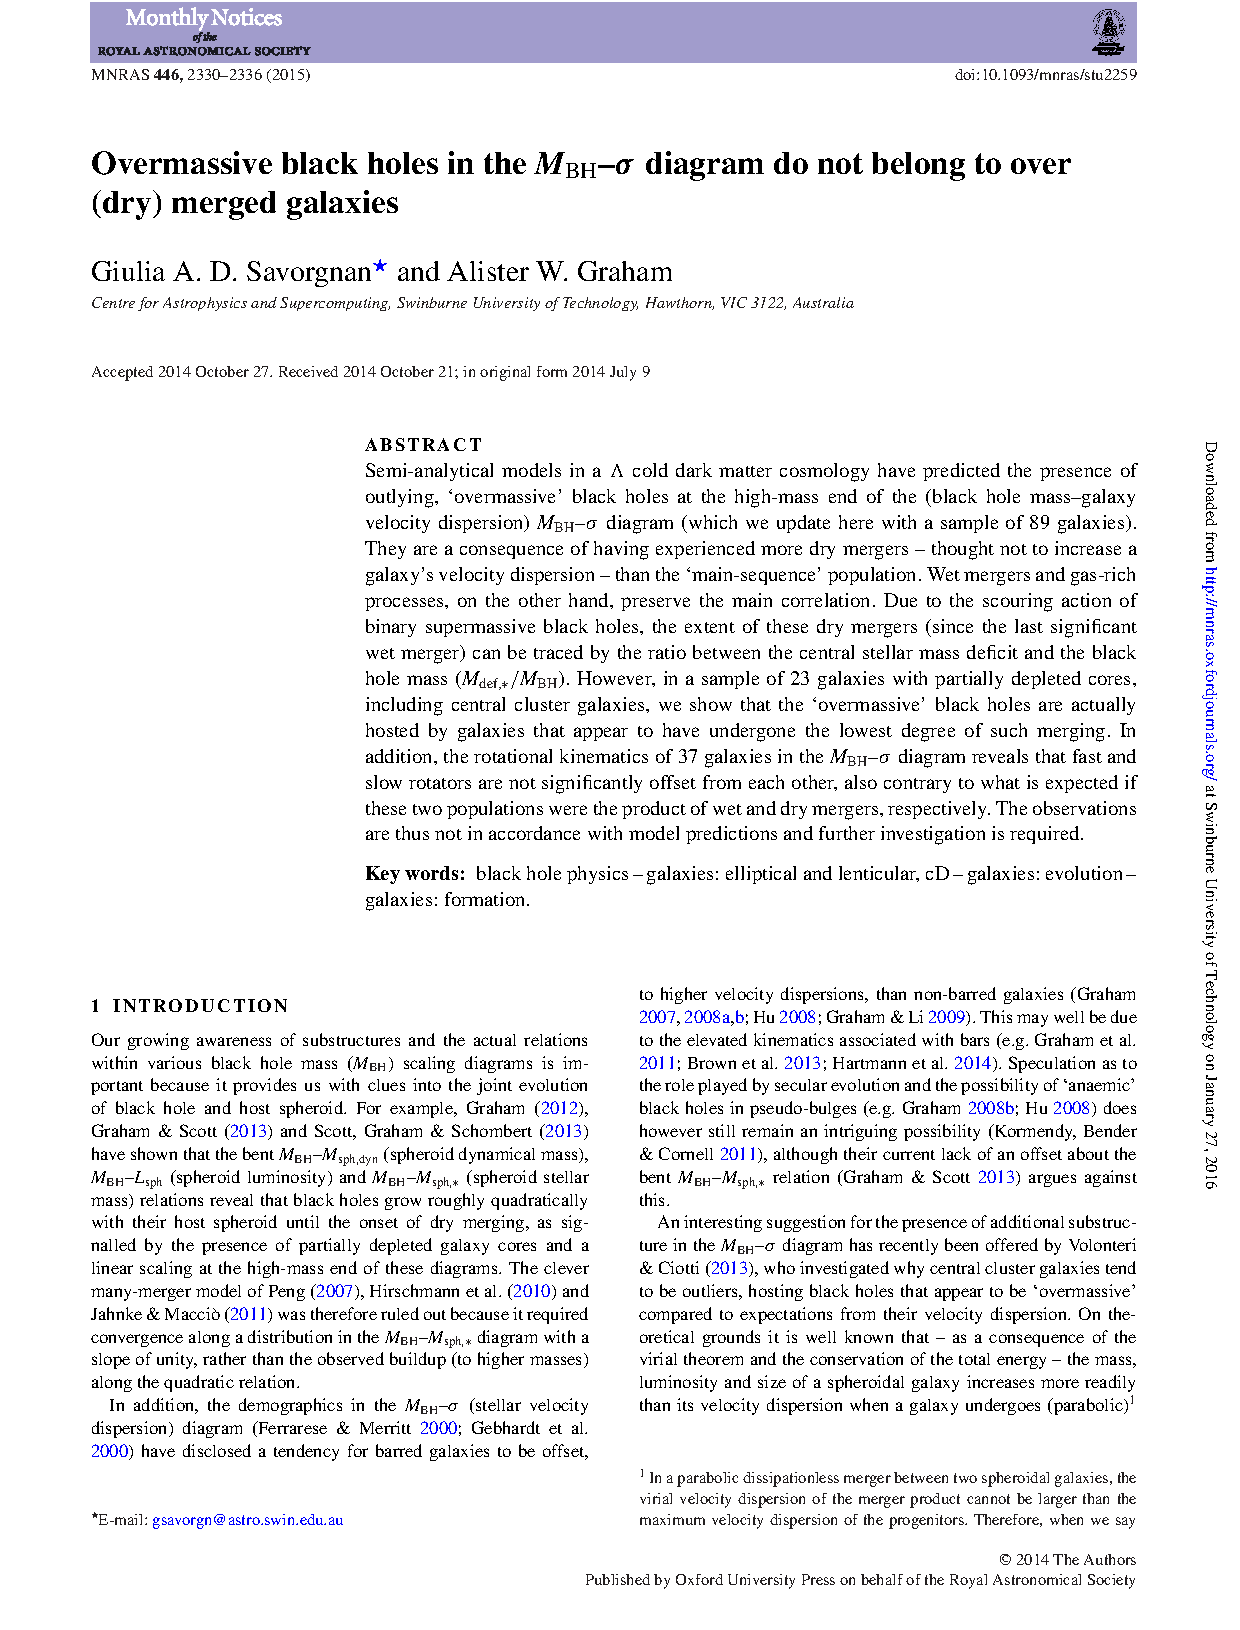
\includepdf[pages={1-7}]{MNRAS2015.pdf}



\documentclass[useAMS,usenatbib,article]{mnras}

\usepackage{longtable}
\usepackage[]{graphicx}
\usepackage{amsmath}
\usepackage{natbib}
\usepackage{soul}
\bibliographystyle{mnras}

%\title[Non over-massive black holes in early-type galaxies]{Early-type galaxies with intermediate-scale discs and their (non over-massive) black holes}
\title[Explaining the reportedly over-massive black holes]
{Explaining the reportedly over-massive black holes in early-type galaxies with intermediate-scale discs}

\author[G.~A.~D. Savorgnan \& A.~W. Graham]
{\parbox{\textwidth}{
Giulia~A.~D. Savorgnan$^{1}$\thanks{E-mail: \texttt{gsavorgn@astro.swin.edu.au}},
Alister W. Graham$^{1}$}\vspace{0.4cm}\\
\parbox{\textwidth}{
$^{1}$Centre for Astrophysics and Supercomputing, Swinburne University of Technology, Hawthorn, Victoria 3122, Australia.\\}}

\pagerange{\pageref{firstpage}--\pageref{lastpage}} \pubyear{2015}

\begin{document}

\maketitle

\label{firstpage}



\begin{abstract}
{\bf The classification ``early-type'' galaxy includes both elliptically- and lenticular-shaped galaxies. 
Theoretically, the spheroid-to-disc flux ratio of an early-type galaxy can assume any positive value,  
but in practice studies often consider only spheroid/disc decompositions 
in which the disc neatly dominates over the spheroid at large galaxy radii, 
creating an inner ``bulge'' as observed in most spiral galaxies. 
Here we show that decompositions in which the disc remains embedded within the spheroid, 
labelled by some as ``unphysical'',  
correctly reproduce both the photometric and kinematic properties of early-type galaxies 
with intermediate-scale discs. 
Intermediate-scale discs have often been confused with large-scale discs and incorrectly modelled as such; 
when this happens, the spheroid luminosity is considerably underestimated. 
This has recently led to some surprising conclusions, 
such as the claim that a number of galaxies with intermediate-scale discs (Mrk 1216, NGC 1277, NGC 1271, and NGC 1332) 
host a central black hole whose mass is abnormally large compared to expectations from the (underestimated) spheroid luminosity. 
We show that when these galaxies are correctly modelled, 
they no longer appear as extreme outliers in the (black hole mass)-(spheroid mass) diagram. 
This not only nullifies the need for invoking different evolutionary scenarios for these galaxies 
but it strengthens the significance of the observed (black hole mass)-(spheroid mass) correlation 
and confirms its importance as a fundamental ingredient for theoretical and semi-analytic models 
used to describe the coevolution of spheroids and their central supermassive black holes. }

\end{abstract}

\begin{keywords}
black hole physics -- galaxies: bulges -- galaxies: elliptical and lenticular, cD -- 
galaxies: evolution -- galaxies: structure -- galaxies: individual: Mrk 1216, NGC 1271, NGC 1277, NGC 1332, NGC 4291
\end{keywords}

\section{Introduction}
\label{sec:int}
{\bf The awareness that \emph{many} early-type galaxies contain previously over-looked stellar discs dates back half a century 
\citep{liller1966,stromstrom1978,michard1984,djorgovski1985,jedrzejewski1987,BenderMoellenhoff1987,
carter1987,capaccioli1987,capaccioli1988}. 
It is well known that 
the identification of a stellar disc in an early-type galaxy, particularly when based on the galaxy's photometric properties, 
is subject to inclination effects. 
As predicted by \cite{carter1987}, this problem is largely overcome with kinematic analyses 
(e.g.~\citealt{franx1989,nieto1991,rixwhite1992,cinzanovandermarel1993,donofrio1995,graham1998fornax}, 
and the ATLAS$^{\rm 3D}$ survey, \citealt{cappellari2011}), 
which allow one to determine the presence of a rotationally-supported component 
in a way nearly insensitive to projection effects \citep{mcelroy1983,cappellari2007,emsellem2007}. 
Yet, identifying the radial extent of an early-type galaxy's disc with respect to the spheroidal component can still be subtle. 
Studying both the surface brightness profiles and the ellipticity profiles 
of early-type galaxies in the Virgo cluster -- including those with elliptical (E), spindle and lenticular (S0) isophotes -- 
\cite{liller1966} drew attention to the observation that many of the galaxies displayed 
``characteristics intermediate between those of type E and type S0'', 
and she classified them as ``ES'' galaxies.  
Building on this and other investigations of ellipticity profiles (e.g.~\citealt{stromstrom1978,ditullio1979}), 
\cite{michard1984} used the classification ``S0-like'' for these early-type galaxies with humped ellipticity profiles, 
dominated by a somewhat edge-on disc at intermediate radii.  
\cite{nieto1988} identified two dozen such spheroid-dominated early-type galaxies, 
whose discs do not prevail at large radii, 
and referred to them as ``disk-ellipticals'' (or ``disky ellipticals'', \citealt{simienmichard1990}).   
However, as noted by \cite{nieto1988}, unless the orientation of the disc is favourable 
(i.e.~somewhat edge-on), it can be missed.  
The same is true when searching for pointy isophotes that are shaped by the combination of the spheroid and a near edge-on disc 
(e.g.~\citealt{carter1978,carter1987,jedrzejewski1987,ebneter1987,BenderMoellenhoff1987,bender1988,bijaoui1989}). \\
Today, most early-type galaxies are classified as ``fast rotators'' 
\citep{atlas3dIII,scott2014}, 
that is, they are rapidly rotating within their half-light radius. 
The exact definition of a fast rotator can be found in \cite{emsellem2007}, 
although the most recent literature (e.g.~\citealt{arnold2011n3115,romanowskyfall2012,arnold2014}) 
prefers the use of the term ``\emph{central} fast rotator'' 
to emphasize the fact that this classification pertains to the kinematic properties of a galaxy only within its half-light radius.
Thanks to their more extended kinematic maps, 
\cite{arnold2014} revealed that some of the central fast rotators continue to be fast rotating at large radii, 
whereas other central fast rotators become slow rotating in their outer regions\footnote{As pointed out by \cite{cappellari2011}, 
while all of the disky ellipticals from \cite{Bender1994} are fast rotators, 
the complement is not true because weak discs only impact the isophotal shape if the discs have orientations close to edge-on, 
whereas their rotational signature can still be detected when they have a near face-on orientation.  
Of course if a disc is face-on, then the galaxy will not be classified as a fast rotator. }.
%A specific angular momentum profile that is rapidly increasing beyond 1--2 half-light radii 
%is a signature of a large-scale disc, 
%while a specific angular momentum profile that increases up to 1--2 half-light radii and then declines beyond that point 
%indicates the presence of an intermediate-scale disc that no longer dominates at large radii. 
Unfortunately, such extended kinematic maps are not yet available for large numbers of galaxies in the local Universe. 
Nevertheless, the ellipticity profile of a galaxy's isophotes can help identify the extent of a stellar disc in an early-type galaxy. \\
In general, stellar discs are intrinsically flat and close to circular (e.g.~\citealt{Andersen2001,AndersenBershady2002}); 
their apparent ellipticity, dictated by their inclination to our line of sight, is fixed. 
Spheroids are often rounder than the observed projection on the sky of their associated discs, 
thus their average ellipticity is often lower than that of their disc. 
An ellipticity profile that increases with radius can be ascribed to an inclined disc that becomes progressively more important at large radii, 
whereas a radial decrease of ellipticity signifies the opposite case. 
This approach can be taken to the next level by inspecting the isophotes for discy structures 
(e.g.~\citealt{carter1978,carter1987,capaccioli1987,jedrzejewski1987,BenderMoellenhoff1987}) 
and checking the velocity line profiles for asymmetry 
(e.g.~\citealt{franxillingworth1988ic1459,bender1990,rixwhite1992,scorzabender1995}, and references therein; \citealt{scorza1998}). \\
Building on the investigations in works such as \cite{liller1966}, \cite{Jedrzejewski1987INPROCEEDINGS} and \cite{rixwhite1990}, 
the toy model shown in Figure \ref{fig:model} illustrates the typical ellipticity profile 
($\epsilon = 1 - b/a$, where $b/a$ is the ratio of minor-to-major axis length) 
and the specific angular momentum profile 
($\lambda = \langle R |V| \rangle / \langle R \sqrt{V^2 + \sigma^2} \rangle$, 
where $R$ is the semimajor-axis radius, $V$ is the mean velocity and $\sigma$ is the velocity dispersion, \citealt{emsellem2007}) 
of: 
(i) a lenticular galaxy, 
comprised of a large-scale disc which dominates the light at large radii over a relatively smaller encased bulge,  
i.e.~a disc-dominated central fast rotator that continues to be fast rotating beyond one half-light radius; 
(ii) a ``discy elliptical'' galaxy \citep{michard1984,nieto1988} 
composed of an intermediate-scale disc embedded in a relatively larger spheroid which dominates the light at large radii,
i.e.~a spheroid-dominated central fast rotator that becomes slow rotating beyond $1-2$ half-light radii; and  
(iii) an elliptical galaxy with an additional nuclear stellar disc, 
i.e.~a (spheroid-dominated) slow rotator. 
This sequence is analogue to that illustrated in Figure 2 of \cite{cappellari2011kmdr}, 
although here we emphasize the correspondence between the spheroid/disc decomposition of the surface brightness profile 
and the ``shape'' of the ellipticity profile (assuming that the disc inclination is not close to face-on) 
and also the specific angular momentum profiles. \\
While some recent studies have correctly distinguished between large- and intermediate-scale discs, 
and modelled them accordingly (e.g.~\citealt{kormendybender2012,krajnovic2013}), 
intermediate-scale discs have been missed by many galaxy modellers of late, 
who have labelled as ``unphysical'' \citep{allen2006} those spheroid/disc decompositions 
in which the disc does not dominate over the spheroid at large radii 
as is observed with spiral galaxies. 
This has led to the rejection of many early-type galaxy decompositions 
similar to that illustrated in the top middle panel of Figure \ref{fig:model}. 
Unsurprisingly, studies affected by this bias have not obtained spheroid/disc decompositions with a spheroid-to-total ratio larger than $0.6 - 0.8$ 
(e.g.~\citealt{gadotti2008,head2014,querejeta2015,mendezabreu2015}). \\
As mentioned before, an isophotal analysis allows one to identify the presence and the radial extent of a disc in an early-type galaxy 
only when the disc has a certain level of inclination. 
On the other hand, a kinematic analysis has the advantage of being virtually insensitive to inclination effects, 
but cannot help one determine the radial extent of a disc if the kinematic data are limited within one half-light radius. 
Therefore, the best results are obtained when photometry and kinematics are combined together. \\
In this paper we focus on the increasingly overlooked occurence of intermediate-scale discs in galaxies with directly measured black hole masses. 
We report on the photometric and kinematical signatures of these intermediate-sized stellar discs,  
and the impact they have on the (black hole mass)-to-(spheroid stellar mass) ratio 
which is used to constrain galaxy evolution models. 
In Section \ref{sec:gal} we present a detailed photometric analysis of three galaxies with intermediate-scale discs (Mrk 1216, NGC 1332, and NGC 3115) 
and we briefly describe another five galaxies with intermediate-scale discs (NGC 821, NGC 1271, NGC 1277, NGC 3377, and NGC 4697) 
already modelled by us elsewhere in the literature. 
We compare our photometric analysis with the kinematical information available from the literature, 
and explain the differences between our galaxy models and past decompositions. 
In Section \ref{sec:mm} we explore the important implications this has for the (black hole mass)-(spheroid stellar mass) diagram. 
Finally, in Section \ref{sec:disc} we briefly discuss our results in terms of galaxy evolution. }




\begin{figure}
\begin{center}
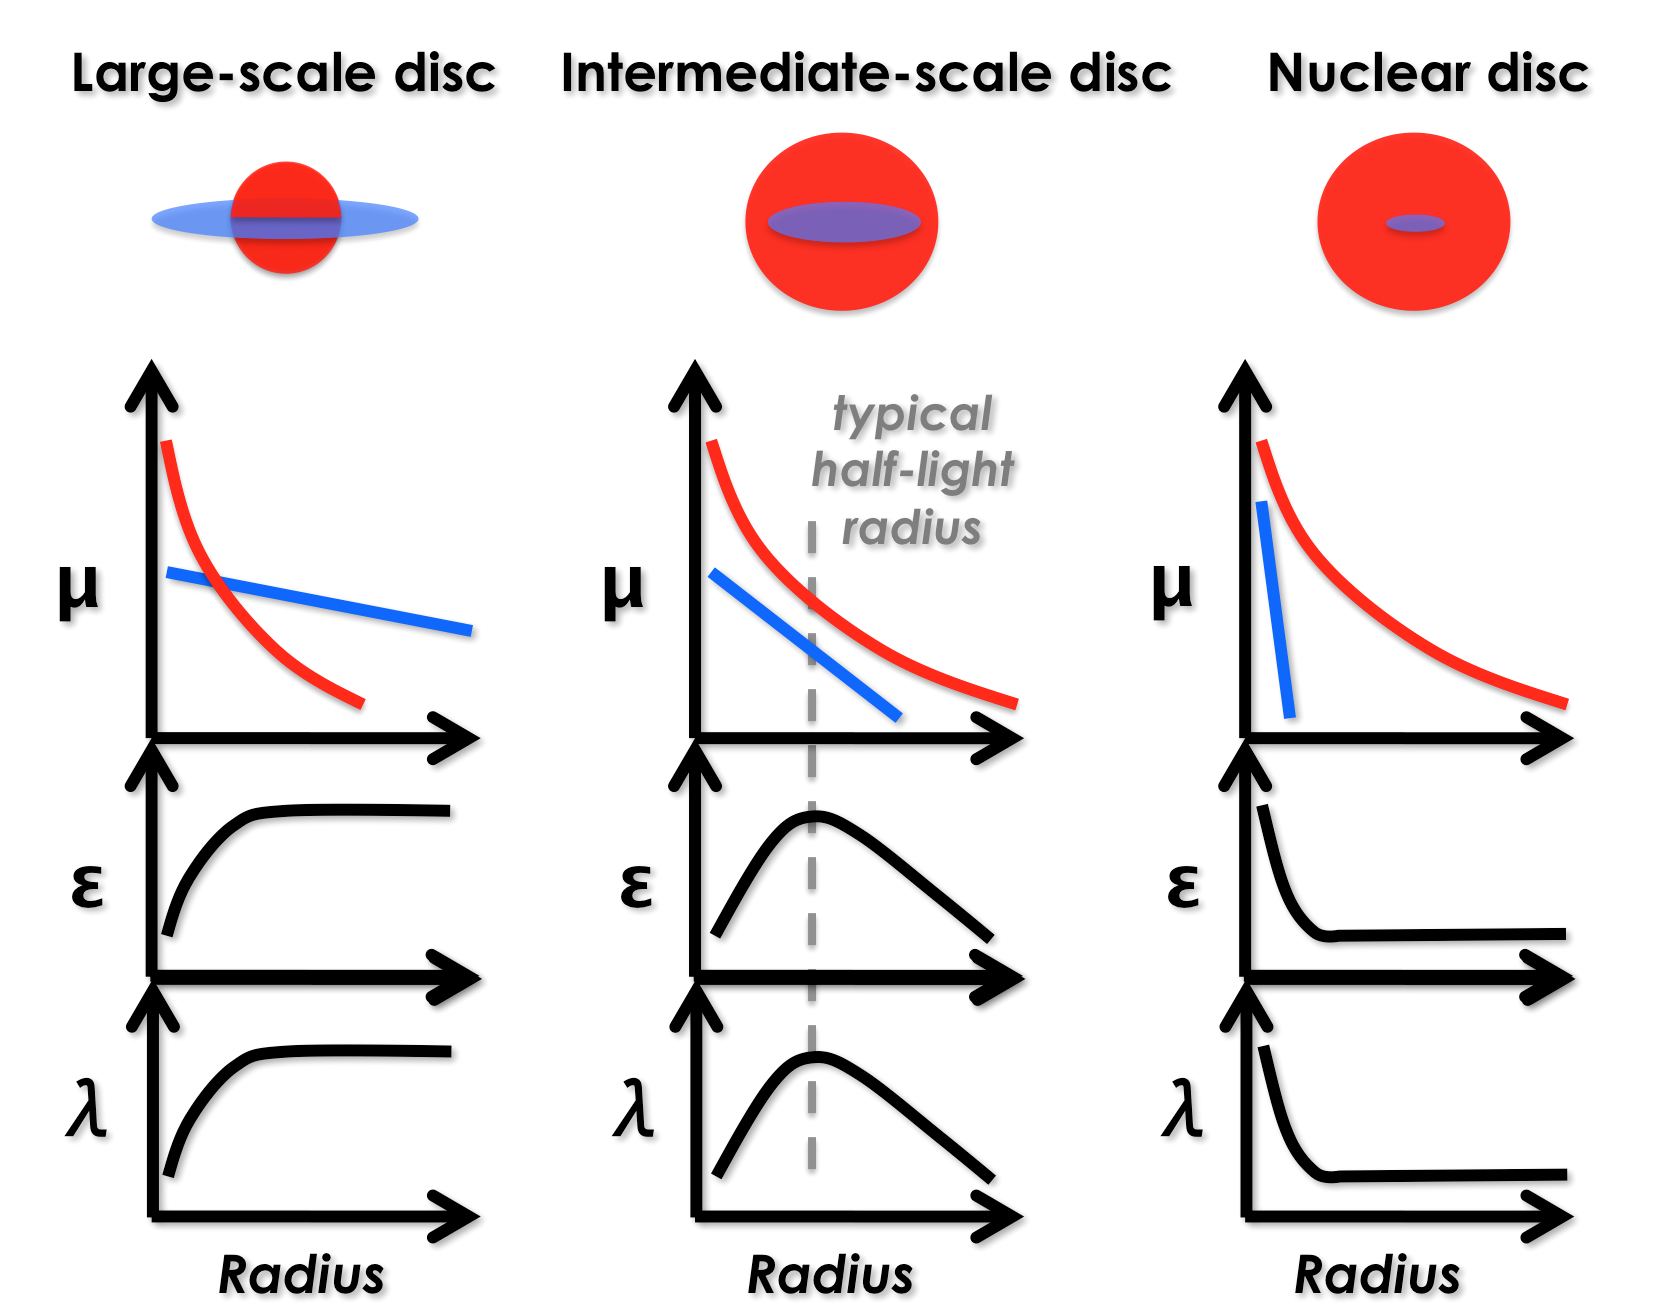
\includegraphics[width=\columnwidth]{discmodel.eps}
\caption{Illustration of the spheroid/disc decomposition of the one-dimensional surface brightness profile, $\mu$, 
the ellipticity profile, $\epsilon$, and the specific angular momentum profile, $\lambda$,
for the three prototype early-type galaxy sub-classes. 
In the flux decompositions, the spheroid (or bulge) and the disc are shown with the red and blue color, respectively. 
The left panel shows a disc-dominated central fast rotator (lenticular galaxy), composed of a bulge encased in a large-scale disc. 
The right panel displays a spheroid-dominated slow rotator (elliptical) with (an optional) nuclear stellar disc. 
The middle panel presents a spheroid-dominated central fast rotator with an intermediate-sized disc embedded in the spheroid. }
\label{fig:model}
\end{center}
\end{figure}


\section{Intermediate-scale disc galaxies}
\label{sec:gal}
Three examples of galaxies with intermediate-scale discs are Mrk 1216, NGC 1332, and NGC 3115. 
In the following Section, we present a photometric analysis of these three galaxies, 
and we compare our results with the kinematical analysis available from the literature for Mrk 1216 and NGC 3115. 
For the galaxies NGC 1332 and NGC 3115, we used $3.6~\rm \mu m$ images obtained with the InfraRed Array Camera (IRAC) 
onboard the \emph{Spitzer Space Telescope}. 
For the galaxy Mrk 1216, we used an archived Hubble Space Telescope (\emph{HST}) image  
taken with the Wide Field Camera 3 (WFC3) and the near-infrared \emph{F160W} filter ($H$-band). 
Our galaxy decomposition technique is extensively described in Savorgnan \& Graham (2015).
Briefly, the galaxy images were background-subtracted, and masks for contaminating sources were created. 
The one-dimensional Point Spread Function (PSF) was characterized using a Gaussian profile for the \emph{HST} observation 
and a \cite{moffat1969} profile for the \emph{Spitzer} observations.
We performed an isophotal analysis of the galaxies using the IRAF\footnote{IRAF 
is the Image Reduction and Analysis Facility, distributed by the National Optical Astronomy Observatory, 
which is operated by the Association of Universities for Research in Astronomy (AURA) 
under cooperative agreement with the National Science Foundation.} task {\tt ellipse}\footnote{Our analysis 
was performed before {\tt isofit} \citep{ciambur2015} was conceived or available. 
After {\tt isofit} was recently developed and implemented in IRAF, 
we employed it to re-extract the surface brightness profiles of the galaxies NGC 1332 and NGC 3115. 
We then repeated the analysis and checked that this change does not significantly alter our results. 
In fact, although {\tt isofit} provides a more accurate description of the isophotes in the presence of an inclined disc, 
the discs of NGC 1332 and NGC 3115 are relatively faint compared to the spheroidal components, 
therefore the differences between the light profile obtained with {\tt ellipse} and that obtained with {\tt isofit} 
are small for these two galaxies. } 
\citep{taskellipse}. 
The galaxy isophotes were modelled with a series of concentric ellipses, 
allowing the ellipticity, the position angle and the amplitude of the fourth harmonic to vary with radius.  
The decomposition of the surface brightness profiles was performed with software written by G. Savorgnan 
and described in Savorgnan \& Graham (2015).
We modelled the light profiles with a combination of PSF-convolved analytic functions, 
using one function per galaxy component. 


\subsection{NGC 3115}
The presence of a disc in the {\bf central fast rotator} NGC 3115 
{\bf (e.g.~\citealt{strom1977,nieto1988,scorzabender1995}) }
is obvious due to its edge-on orientation (Figure \ref{fig:n3115}). 
Less obvious is the radial extent of this disc if one only relies on a visual inspection of the galaxy image. 
The ellipticity profile (Figure \ref{fig:n3115}) is consistent with the presence of an intermediate-scale disc. 
Moreover, the kinematics of NGC 3115 \citep{arnold2011n3115} also disprove the presence of a large-scale disc, 
because the galaxy is rapidly rotating only within two galaxy half-light radii ($\sim 2 \times 50~\rm arcsec$), 
and the rotation significantly drops at larger radii.  
The unsharp mask of NGC 3115 (Figure \ref{fig:n3115}) betrays the presence of a faint edge-on nuclear ring, 
which can also be spotted as a small peak in the ellipticity profile 
(at semi-major axis length $R_{\rm maj} \sim 15~\rm arcsec$). 
Such rings are common in early-type galaxies (e.g.~\citealt{michardmarchal1993}).
The spheroidal component of NGC 3115 is well described with a \cite{sersic1963} profile.
The highly inclined intermediate-scale disc is better fit with an $n<1$ S\'ersic profile 
(the S\'ersic index $n$ regulates the curvature of the S\'ersic profile) 
rather than with an exponential function, 
as explained by \cite{pastrav2013a}. 
The nuclear ring is modelled with a Gaussian function. \\
In comparison, \cite{lasker2014data} fit NGC 3115 with a bulge + disc + envelope, 
and measured a bulge half-light radius of $3.9~\rm arcsec$ and a bulge-to-total ratio of $0.12$. 
We describe this galaxy using a spheroid + intermediate-scale disc + nuclear ring, 
and obtain a spheroid half-light radius of $43.6~\rm arcsec$ and a spheroid-to-total ratio of $0.85$. 
We have used both kinematical information and ellipticity profiles, 
together with the surface brightness profile, 
to obtain a physically consistent and meaningful model. 


\subsection{NGC 1332}
The morphology of NGC 1332 (Figure \ref{fig:n1332}) is very similar to that of NGC 3115, 
with the ellipticity profile indicating the presence of an intermediate-scale disc, 
although in this case no nuclear component is evident. 
We were not able to find any extended kinematic profile or map 
for this galaxy in the literature. 
The data within the innermost $6~\rm arcsec$ were excluded from the fit 
because, according to our galaxy decomposition, they are possibly affected by the presence of a partially depleted core.
The surface brightness profile of NGC 1332 is well described with a S\'ersic-spheroid plus
an $n<1$ S\'ersic-disc. 
Our galaxy decomposition suggests that NGC 1332 is a spheroid-dominated galaxy, 
with a spheroid-to-total ratio of $0.95$. \\
\cite{rusli2011} did not identify the restricted extent of the intermediate-scale disc, 
as revealed by the ellipticity profile, 
and proposed a model featuring a S\'ersic-bulge and a large-scale exponential-disc, 
with a spheroid-to-total ratio of $0.43$.
Based on their bulge/disc decomposition, they concluded that NGC 1332 is a disc-dominated lenticular galaxy 
which is displaced from the (black hole mass)-(spheroid luminosity) correlation of \cite{marconihunt2003} 
by an order of magnitude along the black hole mass direction. 
However, in Section \ref{sec:mm} we show that, according to our decomposition, 
NGC 1332 lies within the $1\sigma$ scatter about the (black hole mass)-(spheroid stellar mass) correlation 
for early-type galaxies. 
We also note that the majority of galaxies with an elevated stellar velocity dispersion ($\sigma > 270~\rm km~s^{-1}$) 
are core-S\'ersic galaxies \citep{graham2003coresersicmodel,ferrarese2006acsvcs,dullograham2014cores}, 
i.e.~they have a partially depleted core which has been identified from high-resolution photometric data. 
NGC 1332 has $\sigma = 320~\rm km~s^{-1}$, but, 
based on their decomposition of \emph{HST} imaging, \cite{rusli2011} did not find a core in this galaxy. 
However, our galaxy decomposition (Figure \ref{fig:n1332}) suggests that NGC 1332 is in fact a core-S\'ersic galaxy. 
Since we did not use high-resolution photometric data, 
we refrain from a firm conclusion, 
but we caution that a re-analysis of the \emph{HST} data -- by taking into account the correct radial extent of the intermediate-scale disc --
may indeed reveal the presence of a depleted core in this galaxy.

\subsection{Mrk 1216}
Although the disc in the {\bf central fast rotator} Mrk 1216 is not immediately apparent from the image (Figure \ref{fig:m1216}), 
the velocity map \citep{yildirim2015} reveals the presence of a fast rotating component 
within three galaxy half-light radii ($\sim 3 \times 5~\rm arcsec$). 
The ellipticity profile (Figure \ref{fig:m1216}), 
which extends out to five half-light radii, indicates the presence of an intermediate-scale disc. 
In addition, a nuclear disc is identified from the change in slope of the ellipticity profile ($R_{\rm maj} \sim 1 - 2 \rm~arcsec$), 
from the unsharp mask, 
and from a clear feature in the $B4$ fourth harmonic profile (not shown here). 
We modelled the surface brightness profile of Mrk 1216 (Figure \ref{fig:m1216}) with a S\'ersic-spheroid, 
an intermediate-sized exponential-disc, and a nuclear exponential-disc. 

\subsection{Other galaxies}
Our models with an intermediate-sized disc embedded within a larger spheroidal component, 
plus an additional nuclear component when one is present, 
match the observed light distribution, and explain both the extended kinematic maps (when available, \citealt{arnold2014}) and the ellipticity profiles, 
of five additional galaxies for which a direct measurement of their central supermassive black hole mass is available: 
NGC 821; NGC 1271; NGC 1277; NGC 3377; and NGC 4697. 
Our isophotal analysis and galaxy decompositions for NGC 1271 and NGC 1277 will be presented in 
Graham, Savorgnan \& Ciambur (\emph{in prep.}) and Graham et al.~(2015), respectively, 
while the galaxies NGC 821, NGC 3377 and NGC 4697 have been analysed in Savorgnan \& Graham (2015). 

\subsubsection{NGC 1271}
\cite{walsh2015} explored a three-component decomposition for the {\bf central fast rotator} NGC 1271 
and identified the galaxy bulge with the innermost of the three components, 
having a half-light radius of $0.61~\rm arcsec$ and a bulge-to-total flux ratio of $0.23$; 
our model features a spheroid + intermediate-scale disc, 
with a spheroid half-light radius of $3.3~\rm arcsec$ and a spheroid-to-total flux ratio of $0.67$. 

\subsubsection{NGC 1277}
\cite{vandenbosch2012} proposed a model for the {\bf central fast rotator} NGC 1277 with a bulge + disc + nuclear source + envelope, 
which gives a bulge half-light radius of $0.9~\rm arcsec$ and a bulge-to-total flux ratio of $0.24$; 
our model consists of a spheroid + intermediate-scale disc + nuclear component, 
and produces a spheroid half-light radius of $6.0~\rm arcsec$ and a spheroid-to-total flux ratio of $0.79$. 

\subsubsection{NGC 3377}
\cite{lasker2014data} modelled the {\bf central fast rotator} NGC 3377 
{\bf (e.g.~\citealt{jedrzejewski1987inproceedings,scorzabender1995}) }
with a bulge + nuclear disc + disc + envelope, 
and obtained a bulge half-light radius of $10.1~\rm arcsec$ and a bulge-to-total flux ratio of $0.35$; 
our model with a spheroid + intermediate-scale disc + nuclear disc 
returns a spheroid half-light radius of $61.8~\rm arcsec$ and a spheroid-to-total flux ratio of $0.94$. 

\subsubsection{NGC 821}
\cite{lasker2014data} decomposed the {\bf central fast rotator} NGC 821 into a bulge + disc + envelope, 
and measured a bulge half-light radius of $3.8~\rm arcsec$ and a bulge-to-total flux ratio of $0.19$; 
our decomposition consists of a spheroid + intermediate-scale disc, 
with a spheroid half-light radius of $36.5~\rm arcsec$ and a spheroid-to-total flux ratio of $0.79$. 

\subsubsection{NGC 4697}
{\bf While NGC 4697 (e.g.~\citealt{carter1987,Jedrzejewski1987n720n1052n4697,davies1981}) 
was explicitly referred to as a ``fast rotator'' by \cite{capaccioli1987} and \cite{petrou1981}, 
it is only a central fast rotator} and it represents an ``extreme'' case. 
\cite{lasker2014data} fit this galaxy with a bulge + nuclear source + disc + envelope, 
and obtained a bulge half-light radius of $6.3~\rm arcsec$ and a bulge-to-total flux ratio of $0.08$; 
we described NGC 4697 using a spheroid + intermediate-scale disc + nuclear disc model, 
and measured a spheroid half-light radius of $239.3~\rm arcsec$ and a spheroid-to-total flux ratio of $0.89$. \\

Past models that ``forcedly'' described intermediate-scale disc galaxies using an inner bulge 
encased within a large-scale disc 
commonly required the addition of an extended envelope or halo to account for the outer portion of the spheroid. 
Such three-component models (bulge + disc + envelope) typically reduce the spheroid luminosity by a factor of $3-4$, 
and underestimate the size of the spheroid by a factor of $6-10$, 
although more ``extreme'' cases can be found. 


\begin{figure}
\begin{center}
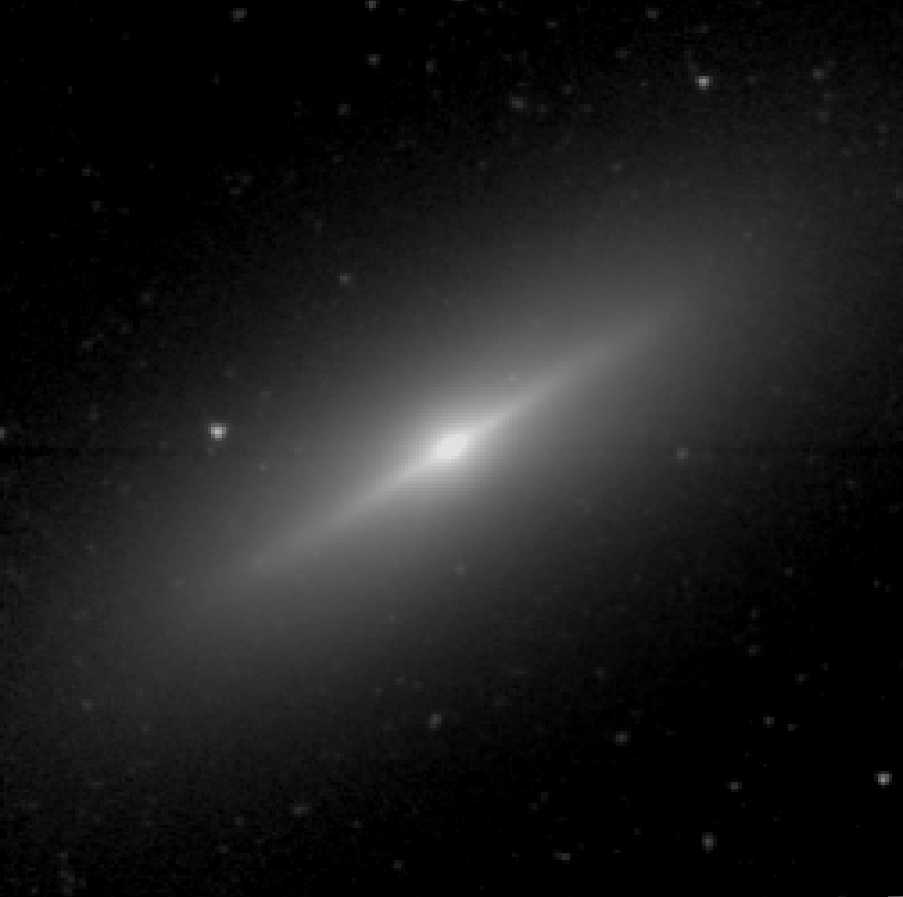
\includegraphics[width=0.49\columnwidth]{n3115_image.jpeg}
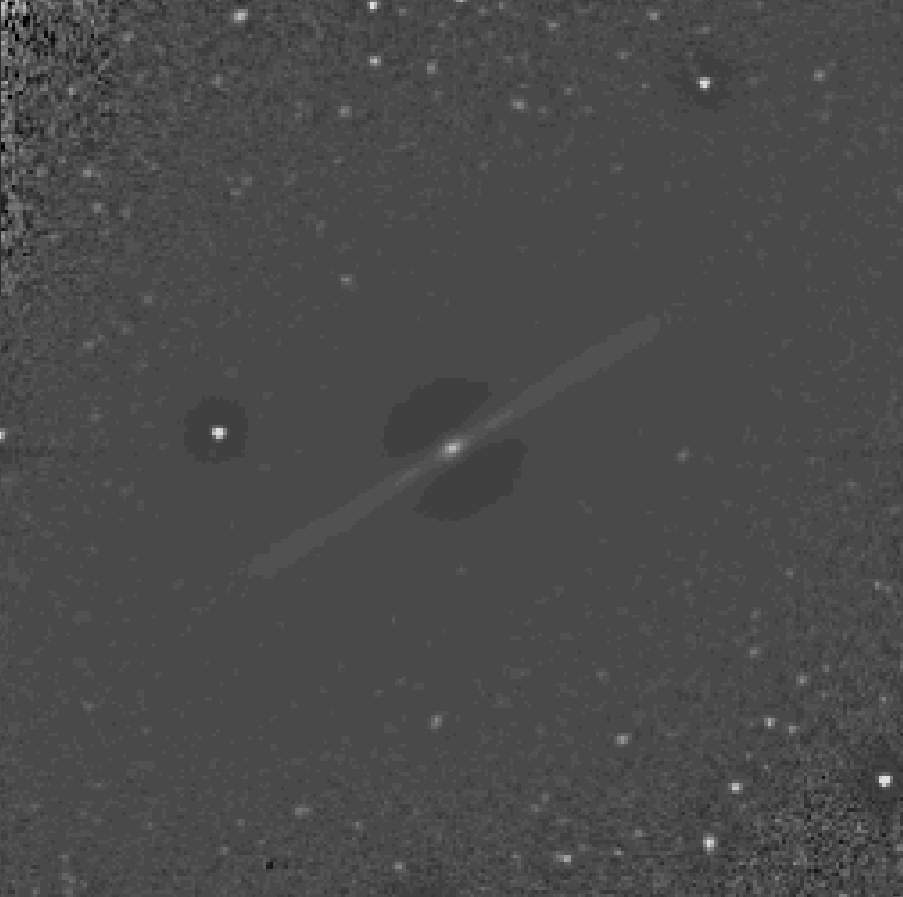
\includegraphics[width=0.49\columnwidth]{n3115_unsharp.jpeg} \\
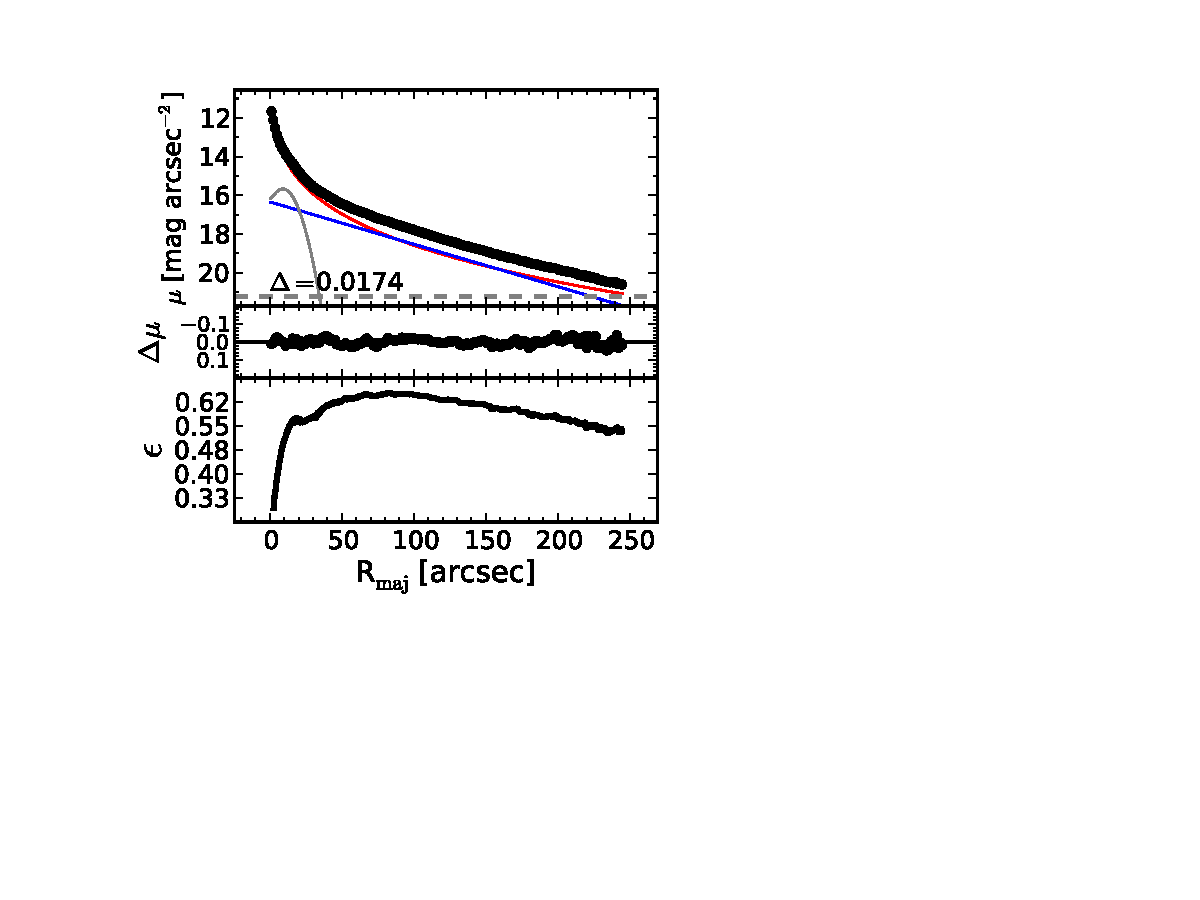
\includegraphics[width=1.05\columnwidth]{n3115_decomposition.pdf}
\caption{NGC 3115. 
The top panels are the \emph{Spitzer}/IRAC $3.6~\rm \mu m$ image (left) and its unsharp mask (right), 
obtained by dividing the image by a Gaussian-smoothed version of itself. 
The bottom plots display the best-fit model of the surface brightness profile, $\mu$, 
and the ellipticity profile, $\epsilon$, 
along the major-axis, $R_{\rm maj}$. 
The black points are the observed data, which extend out to five galaxy half-light radii ($\sim 5 \times 50~\rm arcsec$). 
The color lines represent the individual (PSF-convolved) model components: 
{\bf red solid = S\'ersic (spheroid), blue dashed = S\'ersic (disc), green dotted = Gaussian ring. }
The residual profile (data $-$ model) is shown as $\Delta \mu$. 
The horizontal gray dashed line corresponds to an intensity equal to three times the root mean square of the sky background fluctuations. 
$\Delta$ denotes the root mean square scatter of the fit in units of $\rm mag~arcsec^{-2}$. }
\label{fig:n3115}
\end{center}
\end{figure}

\begin{figure}
\begin{center}
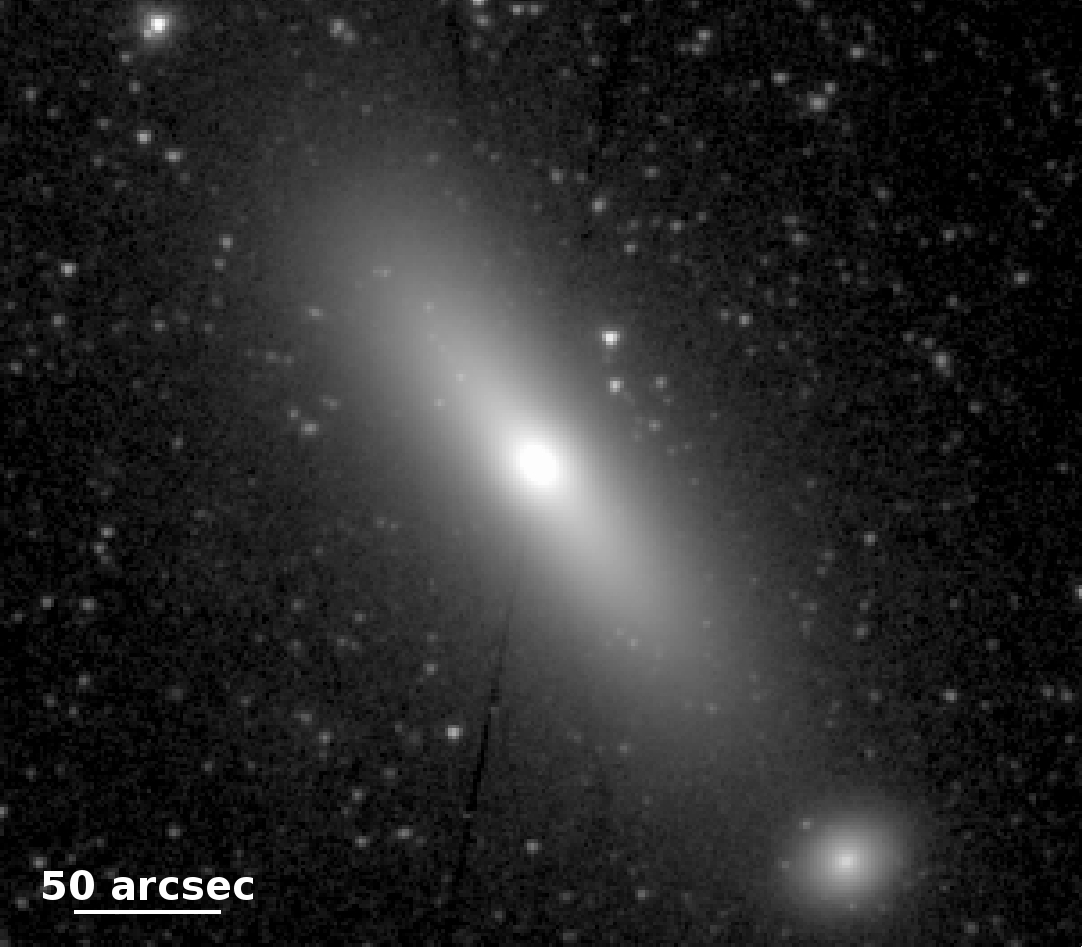
\includegraphics[width=0.49\columnwidth]{n1332_image}
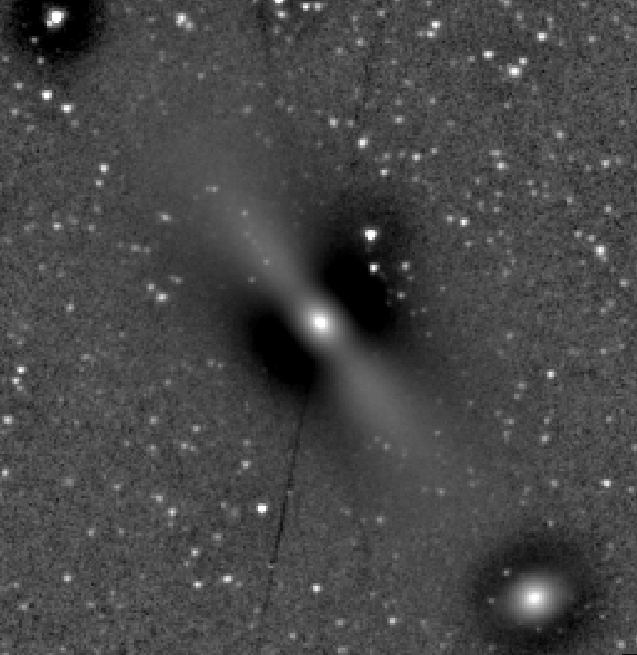
\includegraphics[width=0.49\columnwidth]{n1332_unsharp} \\
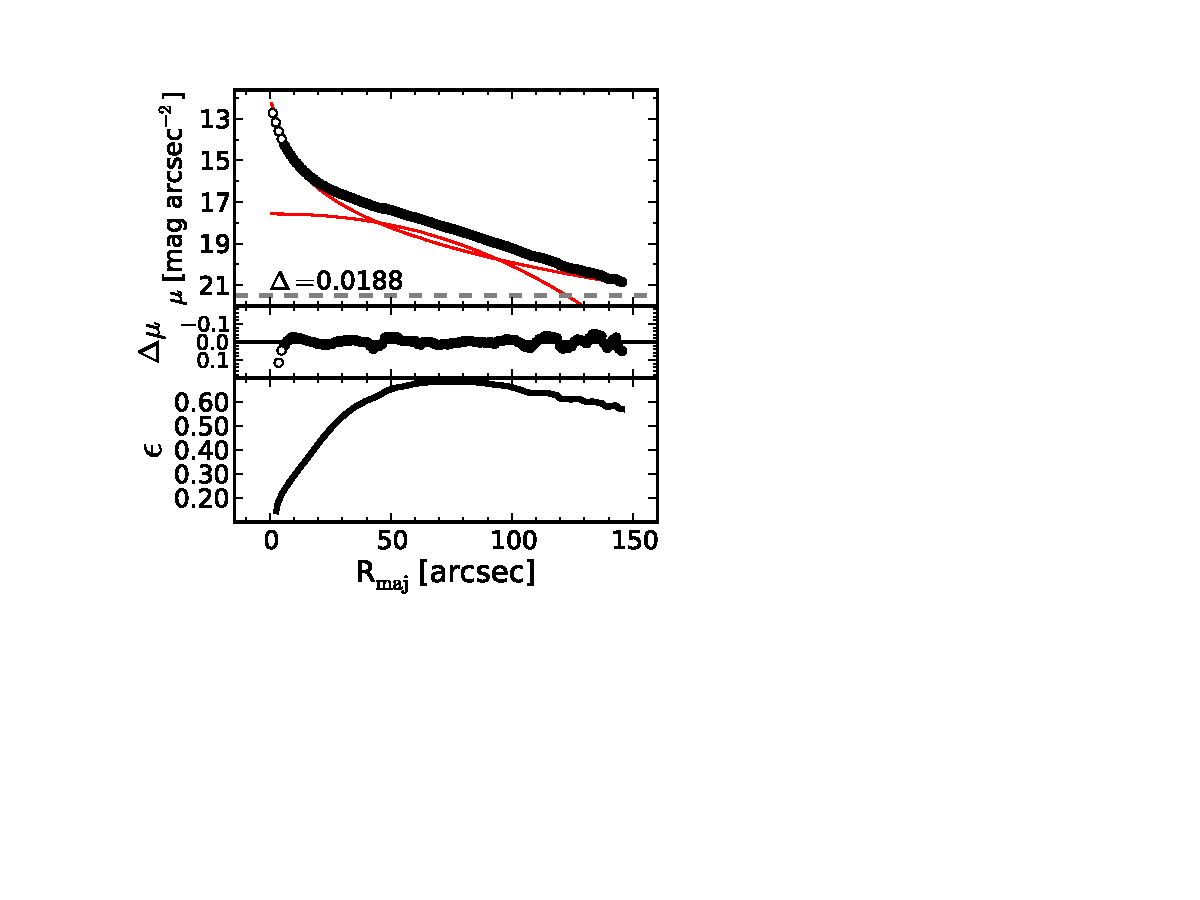
\includegraphics[width=1.03\columnwidth]{n1332_decomposition.pdf}
\caption{NGC 1332.
Similar to Figure \ref{fig:n3115}. 
The surface brightness profile extends out to seven galaxy half-light radii ($\sim 7 \times 20~\rm arcsec$). 
The empty points are data excluded from the fit. 
}
\label{fig:n1332}
\end{center}
\end{figure}

\begin{figure}
\begin{center}
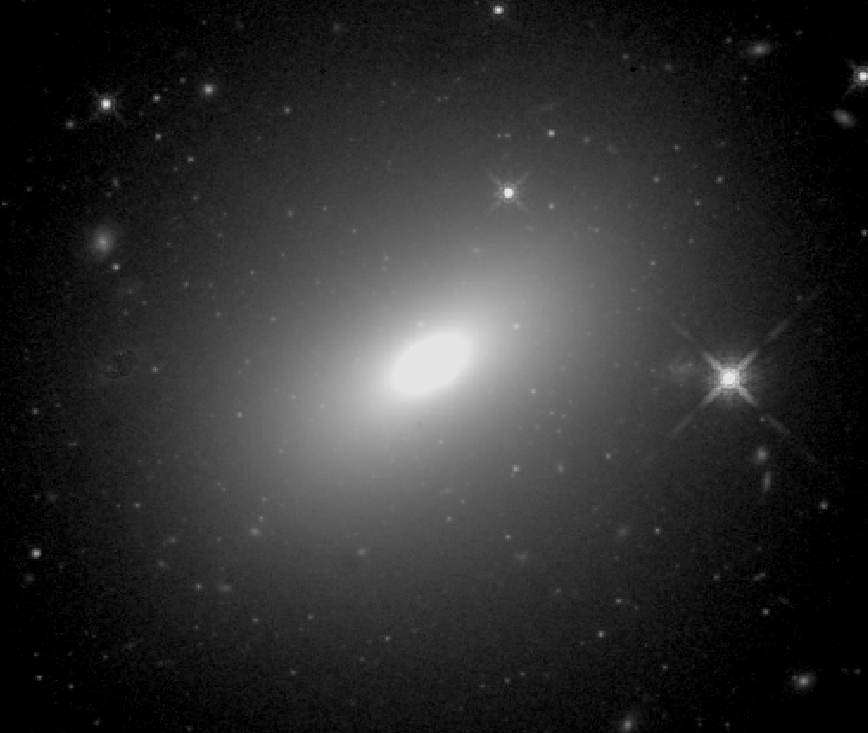
\includegraphics[width=0.49\columnwidth]{mrk1216_image.jpeg}
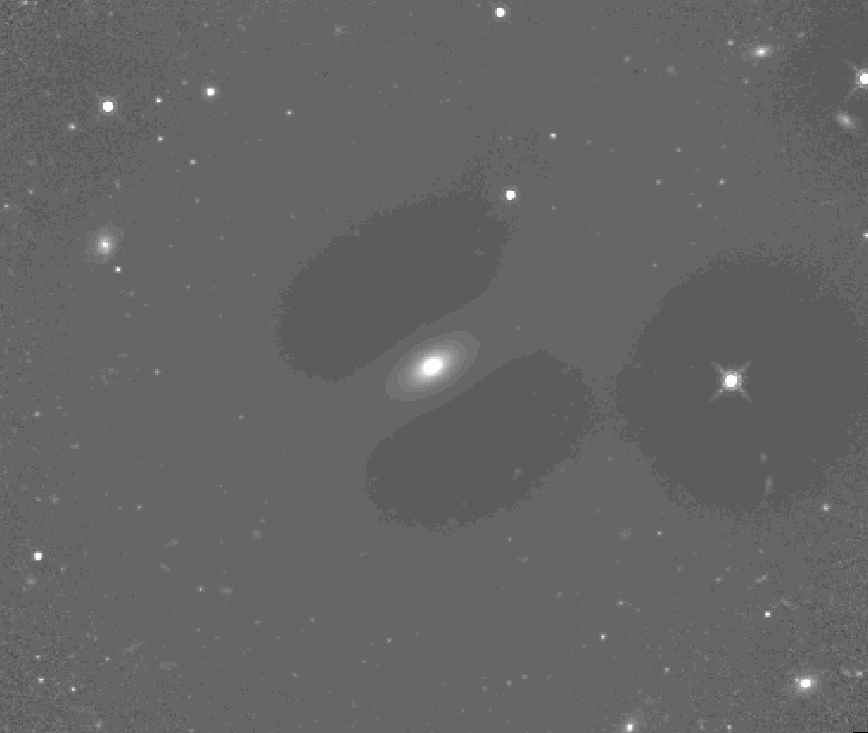
\includegraphics[width=0.49\columnwidth]{mrk1216_unsharp.jpeg} \\
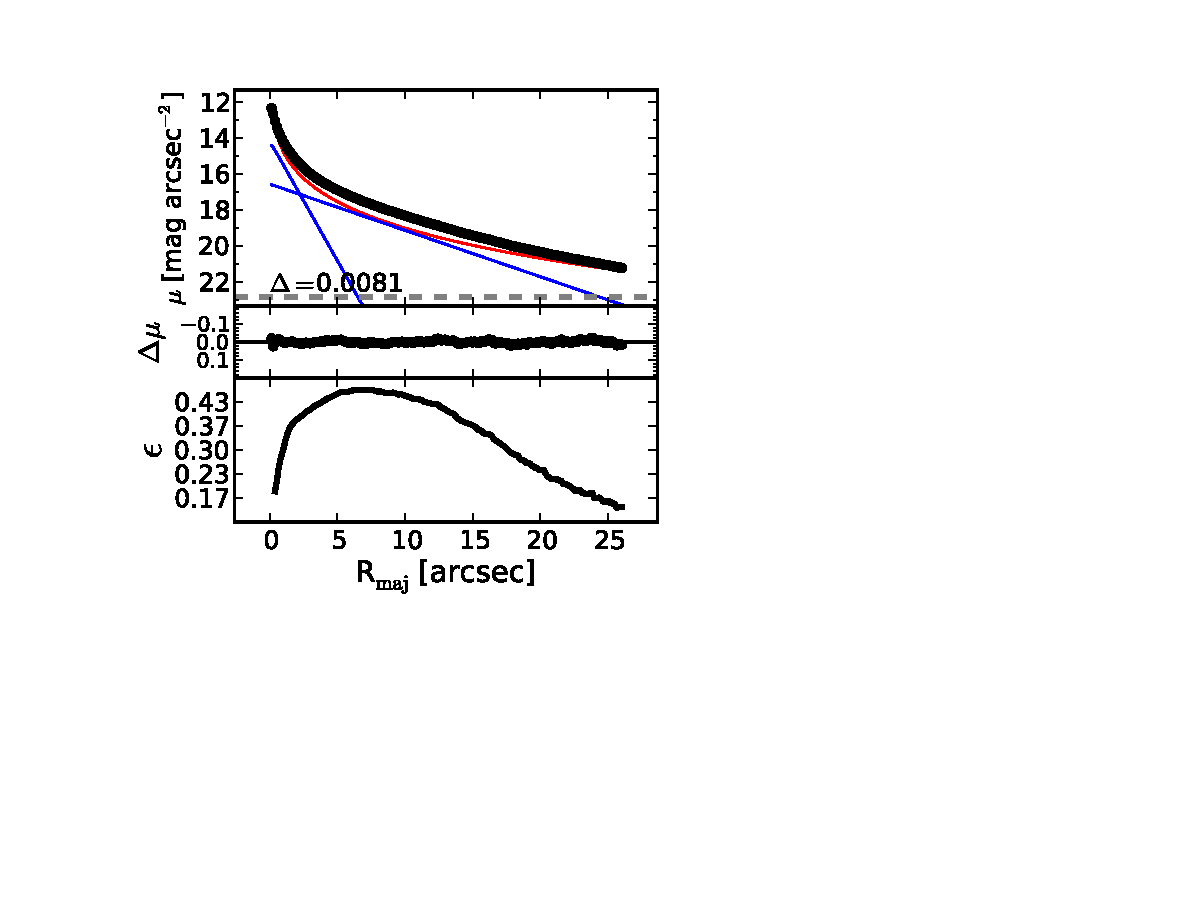
\includegraphics[width=1.05\columnwidth]{mrk1216_decomposition.pdf}
\caption{Mrk 1216. 
Similar to Figure \ref{fig:n3115}. 
The top panels are the \emph{HST}/WFC3 \emph{F160W} image (left) and its unsharp mask (right).
The surface brightness profile extends out to five galaxy half-light radii ($\sim 5 \times 5~\rm arcsec$). 
The color lines represent the individual (PSF-convolved) model components:
{\bf red solid = S\'ersic (spheroid), blue dashed = exponential (nuclear and intermediate-scale disc). }
}
\label{fig:m1216}
\end{center}
\end{figure}



\section{The black hole -- spheroid correlation}
\label{sec:mm}
Inaccurate measurements of the spheroid-to-total ratio of galaxies can impact galaxy scaling relations. 
Recently, a handful of galaxies with intermediate-scale discs have been claimed to host \emph{over-massive} black holes, 
i.e.~the mass of their central supermassive black hole has been reported to be significantly larger 
than what is expected from the galaxy's spheroid luminosity (or stellar mass).
This is the case for the galaxies Mrk 1216 (for which only an upper limit on its black hole mass has been published, 
\citealt{yildirim2015}), NGC 1271 \citep{walsh2015}, 
NGC 1277 \citep{vandenbosch2012,yildirim2015} and NGC 1332 \citep{rusli2011}.
In addition to these, the elliptical galaxy NGC 4291 has also been claimed to be a $\sim$$3.6\sigma$ outlier 
above the (black hole mass)-(spheroid mass) scaling relation \citep{bogdan2012}. 
Obviously, having both the black hole mass and the spheroid mass correct is important 
for placing systems in the (black hole mass)-(spheroid mass) diagram. \\
\emph{At present, for early-type galaxies, the spheroid luminosity and the galaxy luminosity 
can be used to predict the black hole mass with the same level of accuracy\footnote{Note that 
\cite{lasker2014anal} reported that the spheroid luminosity and the galaxy luminosity are equally good tracers of the black hole mass 
irrespective of the galaxy morphological type, but their sample of 35 galaxies contained only 4 spiral galaxies. 
However, using a sample of 45 early-type and 17 spiral galaxies, 
Savorgnan et al.~(2015) shows that, when considering all galaxies irrespective of their morphological type, 
the correlation of the black hole mass with the spheroid luminosity is better than that with the galaxy luminosity.} 
(Savorgnan et al.~2015). 
If a galaxy hosts a black hole that is over-massive compared to expectations from the spheroid luminosity, 
but whose mass is normal compared to expectations from the galaxy luminosity, 
one should wonder whether the spheroid luminosity might have been underestimated 
due to an inaccurate spheroid/disc decomposition. }
Indeed, none of the five galaxies just mentioned (Mrk 1216, NGC 1271, NGC 1277, NGC 1332, and NGC 4291) is a noticeable outlier 
in the (black hole mass)-(galaxy luminosity) diagram. 
In Figure \ref{fig:mm} we show the location of these five galaxies in the updated (black hole mass)-(spheroid stellar mass) diagram 
for early-type galaxies from Savorgnan et al.~(2015). 
Figure \ref{fig:mm} was populated using the galaxy decomposition technique shown here 
and extensively described in Savorgnan \& Graham (2015). 
Briefly, we obtained Spitzer/IRAC $3.6~\rm \mu m$ images for 45 early-type galaxies 
which already had a dynamical detection of their black hole mass. 
We modelled their one-dimensional surface brightness profiles with a combination of analytic functions, 
using one function per galaxy component. 
Spheroid luminosities were converted into stellar masses using individual, 
but almost constant mass-to-light ratios ($\sim$$0.6$, \citealt{meidt2014}). \\
In Figure \ref{fig:mm}, we show the galaxies Mrk 1216, NGC 1271 and NGC 1277, 
which were not a part of the original sample of 45 early-type galaxies.
For the galaxy NGC 1271, we use the black hole mass measurement 
and the stellar mass-to-light ratio obtained by \cite{walsh2015}. 
For the galaxy NGC 1277, we use the black hole mass measurement obtained by \cite{vandenbosch2012} 
and the stellar mass-to-light ratio obtained by \cite{martinnavarro2015}. 
For the galaxy Mrk 1216, we use the upper limit on the black hole mass 
and the stellar mass-to-light ratio obtained by \cite{yildirim2015}. 
For the first time, Figure \ref{fig:mm} reveals that when the four intermediate-scale disc galaxies Mrk 1216, NGC 1271, NGC 1277, NGC 1332, 
and the elliptical galaxy NGC 4291 are properly modelled, 
they no longer appear as extreme outliers above the (black hole mass)-(spheroid stellar mass) correlation for early-type galaxies, 
i.e.~they all reside well within a $3\sigma$ deviation from the correlation.


\section{Origin of compact massive galaxies}
\label{sec:disc}

Acknowledging the correct structure of galaxies with intermediate-scale discs is important to properly understand their origin. 
According to the current paradigm of cosmological structure evolution, 
the genesis of massive early-type galaxies is characterized by two distinct phases: ``in-situ'' and ``ex-situ''. 
The first phase takes place in a young Universe (within its first $4~\rm Gyr$), 
when cold gas inflows produced short and intense bursts of star formation 
that created compact and dense conglomerates of stars with high velocity dispersion (e.g.~\citealt{prieto2013}). 
These naked and compact conglomerates, named ``red nuggets'' \citep{damjanov2009}, 
have been observed at high-redshift with half-light sizes of 1--2 kpc \citep{daddi2005,trujillo2006,vandokkum2008}.
In the second phase (last $10~\rm Gyr$), discs and stellar envelopes 
were accreted around these primordial conglomerates and the external parts of today's galaxies assembled on scales of 2--20 kpc 
(e.g.~\citealt{driver2013}). \\
Today's Universe is populated by an abundance of compact, massive spheroids, 
with the same physical properties -- mass and compactness -- as the high-redshift red nuggets \citep{GDS2015}. 
Some of these local compact massive spheroids are encased within a large-scale disc, 
that is to say they are the bulges of some lenticular and spiral galaxies.  
Over the last $10~\rm Gyr$ their spheroids have evolved by growing a relatively flat disc (e.g.~\citealt{pichon2011,danovich2012,stewart2013})
-- rather than a three-dimensional envelope -- 
which has increased the galaxy size but preserved the bulge compactness. 
{\bf Of course some lenticular/ES galaxies may have been built from mergers (e.g.~\citealt{querejeta2015}, and references therein). }
The other compact massive spheroids of today's Universe belong to some galaxies with intermediate-scale discs. 
Indeed, Mrk 1216, NGC 1271, NGC 1277, NGC 1332, and NGC 3115 are all local compact intermediate-scale disc galaxies 
with purely old ($>10~\rm Gyr$) stellar populations. 
These galaxies have undergone the lowest degree of disc growth. \\
In addition to the observational clues as to the actual physical components in galaxies with intermediate-scale discs, 
one can reason on other grounds as to why these compact galaxies are not comprised of an inner bulge 
plus large-scale disc plus outer envelope. 
If they were such three-component systems, then one would have two possibilities. 
The first possibility is that these galaxies were already fully assembled $10~\rm Gyr$ ago; 
this would explain their old stellar populations, 
but it would also imply that their discs and envelopes had already formed during the first $4~\rm Gyr$ of the Universe, 
in disagreement with the current cosmological picture. 
The second possibility is that only their inner bulges (with sizes of 0.1--0.2 kpc, 
according to past decompositions) originated in the first $4~\rm Gyr$ 
and they subsequently accreted a substantial disc and envelope. 
If this was correct, then we would observe high-redshift, star-like, naked bulges with stellar masses 
within a factor of a few times the currently observed red nuggets but sizes which are $10$ times smaller. 
However, a dramatically different expectation is reached 
if one considers these galaxies today as spheroid-dominated systems with an intermediate-scale disc; 
in this case, both the galaxy size and the spheroid size are compact (1--2 kpc). 
This implies that, among the local descendants of the high-redshift red nuggets, 
the compact intermediate-scale disc galaxies have undergone the lowest degree of disc growth. 
That is, the bulk of a compact intermediate-scale disc galaxy quickly assembled ``in-situ'' in a very young Universe 
and experienced very little evolution over the last $10~\rm Gyr$.

\begin{figure}
\begin{center}
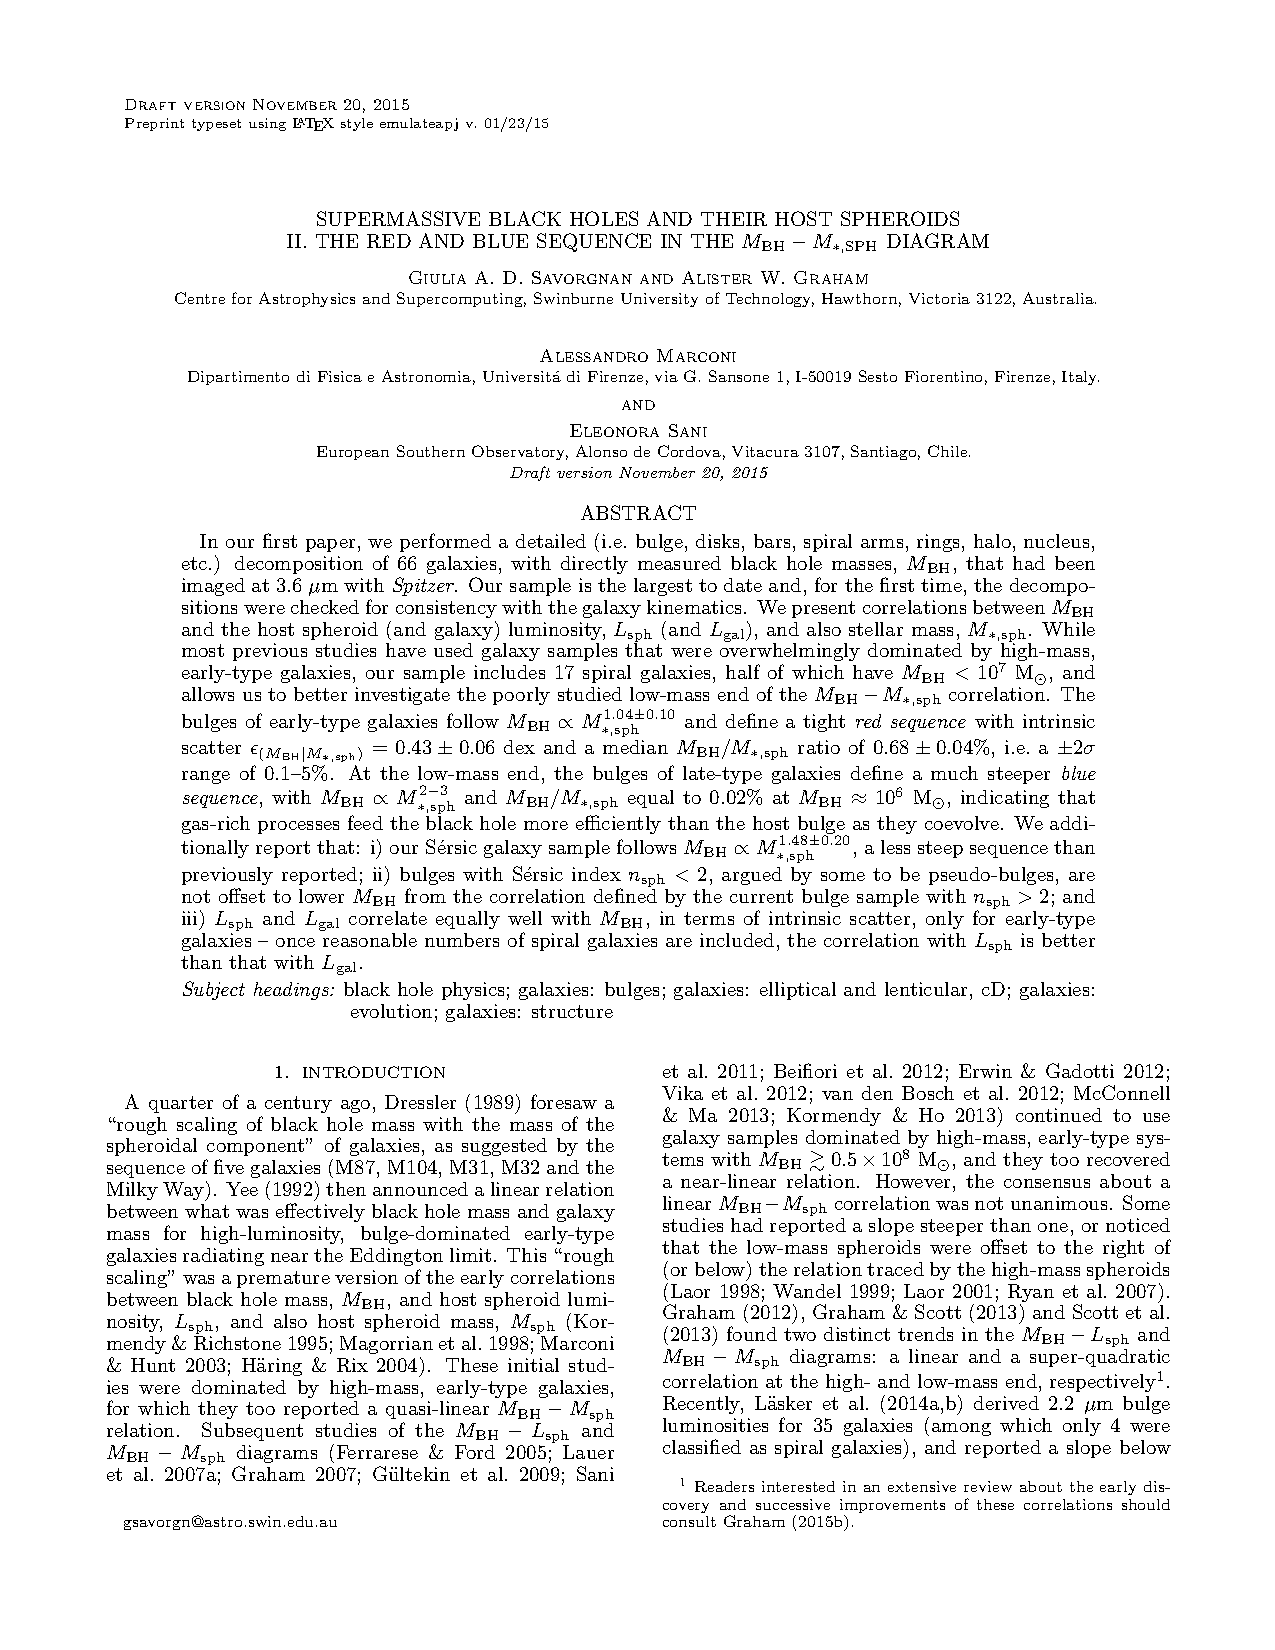
\includegraphics[width=\columnwidth]{mm.pdf}
\caption{Black hole mass plotted against spheroid stellar mass for 45+3 early-type galaxies (from Savorgnan et al.~2015). 
The black solid line is the bisector linear regression for all galaxies except Mrk 1216, NGC 1271 and NGC 1277. 
The dashed lines mark the $1\sigma$ and $3\sigma$ deviations, 
where $\sigma$ ($0.51$ dex) is the total \emph{rms} scatter about the correlation in the black hole mass direction. 
The red symbols mark five galaxies that were claimed to be extreme outliers in this diagram: 
four intermediate-scale disc galaxies (Mrk 1216, NGC 1271, NGC 1277 and NGC 1332) and one elliptical galaxy (NGC 4291). 
All five reside well within a $3\sigma$ deviation from the correlation when using their correct spheroid mass. 
For NGC 1277, we show the previously reported spheroid stellar mass \citep{vandenbosch2012} in gray. 
The green color is used to show the location of four additional intermediate-scale disc galaxies mentioned in Section \ref{sec:gal}.}
\label{fig:mm}
\end{center}
\end{figure}



\section{Summary and conclusions}
{\bf Early-type galaxies display a broad distribution of spheroid-to-total flux ratios (e.g.~\citealt{cappellari2011kmdr}), 
going from disc-less, ``pure'' elliptical galaxies (slow rotators) 
to disc-dominated lenticular galaxies (central fast rotators that continue to be fast rotating also beyond one half-light radius). 
In between these two extremes lie galaxies with intermediate-scale discs 
(spheroid dominated central fast rotators that become slow rotating in their outer regions), 
i.e.~discs of kiloparsec-size that remain ``embedded'' within the spheroidal component of the galaxy 
and do not dominate the galaxy light at large radii as large-scale discs do. }
While this is likely known to some readers, 
the surge of papers presenting galaxy decompositions which are not aware of this reality 
has created a pressing need for this reminder. 
We have shown that the light distribution of galaxies with intermediate-scale discs can be accurately described 
with a simple spheroid + disc (+ optional nuclear component) model, 
without the need for the addition of a bright envelope-component. \\
Our decompositions correctly reproduce both the photometric (surface brightness and ellipticity profiles) 
and kinematic (specific angular momentum profile) properties of nine intermediate-scale disc galaxies. 
Four of these nine galaxies (Mrk 1216, NGC 1271, NGC 1277, NGC 1332) and one additional elliptical galaxy (NGC 4291) 
had previously been claimed to be extreme outliers in the (black hole mass)-(spheroid mass) diagram. 
However, here we have demonstrated that, when correctly modelled, 
these five galaxies all reside well within the scatter of the correlation, 
i.e. they do not host over-massive black holes. 
This serves to strengthen the (black hole mass)-(spheroid mass) relation, 
and rules out the need for exotic formation scenarios. 

\section{Acknowledgments}
This research was supported by Australian Research Council funding through grant FT110100263. 
GS is grateful to Matteo Fossati, Luca Cortese and Giuseppe Gavazzi for useful comments and discussion. 
The publication of this paper would not have been possible without the invaluable support of 
Chris Blake and Duncan Forbes. 
We warmly thank our anynimous referee for their very careful review of our paper, 
and for the comments, corrections and suggestions that ensued. 
This work is based on observations made with the IRAC instrument \citep{fazio2004IRAC} on-board the Spitzer Space Telescope, 
which is operated by the Jet Propulsion Laboratory, California Institute of Technology under a contract with NASA, 
and also on observations made with the NASA/ESA Hubble Space Telescope, 
and obtained from the Hubble Legacy Archive, 
which is a collaboration between the Space Telescope Science Institute (STScI/NASA), 
the Space Telescope European Coordinating Facility (ST-ECF/ESA) and the Canadian Astronomy Data Centre (CADC/NRC/CSA).
This research has made use of the GOLDMine database \citep{goldmine} and the NASA/IPAC Extragalactic Database (NED) 
which is operated by the Jet Propulsion Laboratory, California Institute of Technology, 
under contract with the National Aeronautics and Space Administration. 

%\bibliography{/Users/gsavorgnan/galaxy_vivisection/papers/SMBHbibliography}
\bibliography{SMBHbibliography}


\label{lastpage}

\clearpage


\end{document}


\chapter{Final remarks}
\label{ch:concl}

In this thesis, we explored scaling relations between the supermassive black hole mass 
and various properties of the host spheroid, 
aiming at gaining a more profound understanding of the co-evolution between SMBHs and galaxies. 
A summary of our principal findings and some additional brief considerations about them are presented here. 
The end of this Chapter incorporates some promising future research directions. \\

In Chapter \ref{ch:recov-mn} \citep{savorgnan2013}, we compared the results obtained by four independent studies 
\citep{grahamdriver2007,sani2011,vika2012,beifiori2012}
that attempted photometric decompositions of similar samples of galaxies with a direct measurement 
of the black hole mass. 
In many cases we found a large discrepancy between the S\'ersic index measurements 
obtained by different studies for the spheroidal component of the same galaxy, 
either due to a significantly different choice of model components 
or to other various systematic effects. 
By rejecting the most discrepant S\'ersic index measurements and averaging the remaining ones, 
we were able to recover a strong $M_{\rm BH} - n_{\rm sph}$ correlation, 
which was not found using the individual datasets of three of the four studies. 
From this we concluded that some of the galaxy decompositions were not accurate. 
Chapter \ref{ch:recov-mn} emphasises the importance of a correct, physically motivated selection of model components 
and cautions against the several systematics that can affect galaxy decomposition. \\

Chapter \ref{ch:galviv} was dedicated to the careful multicomponent decomposition of 66 galaxies 
with a direct measurement of the black hole mass. 
We followed the same approach as \citet{laurikainen2005} in selecting the components for each galaxy model.  
\emph{A priori} identification of the galaxy components was done on the basis of several different indicators 
such as the analysis of the isophotal parameters, 
the inspection of unsharp masks, 
complementary information extracted from the literature, 
and -- most importantly -- from the galaxy kinematics. 
A joint photometric-kinematic approach (e.g.~\citealt{krajnovic2013,arnold2014}) 
turned out to play a decisive role for the robustness of our galaxy modelling. 
Upon examining central \citep{atlas3dIII,scott2014} and more extended \citep{arnold2014} velocity maps 
and comparing kinematic and photometric signatures of stellar discs, 
we were able to securely identify the presence and the radial extent of such discs. 
We observed a wide range of spheroid-to-disc ratios in early-type galaxies, 
going from parsec-sized nuclear discs, to kiloparsec-sized intermediate- and large-scale discs, 
in agreement with the findings of \citet{krajnovic2013}. 
Comparison of our results with those obtained by previous studies indicates that 
multicomponent models (as opposed to simple bulge/disc models) are necessary 
to derive reliable structural parameters, confirming previous results 
(e.g.~\citealt{laurikainen2005,laurikainen2007,laurikainen2010,lasker2014data,salo2015}). 
In general, the best-fit parameters obtained with 1D and 2D decomposition techniques for the same galaxy 
are consistent with each other, 
i.e.~no systematic effects were noticed between 1D and 2D modelling. 
However, our practical experience led us to prefer the 1D decomposition technique. 
Advantages associated with the 1D technique are a higher convergence rate for the fits, 
the wealth of information contained in the 1D isophotal analysis, 
and the easier interpretation of the 1D residuals. 
We caution against the dangerous practice of identifying unsubtracted galaxy components 
from the residual image of a 2D fit. 
As an additional warning, 
given the level of detail to which our galaxy decompositions were carried out, 
we do not consider possible for current automatic routines to reproduce our analysis. \\

In Chapter \ref{ch:mm}, we used our dataset to derive and explore 
the $M_{\rm BH} - L_{\rm gal}$ and $M_{\rm BH} - L_{\rm sph}$ (or $M_{\rm BH} - M_{\rm *,sph}$) relations. 
We identified two distinct trends in the $M_{\rm BH} - M_{\rm *,sph}$ diagram, 
that is, a \emph{red sequence} of early-type galaxies (E+S0) 
following $M_{\rm BH} \propto M_{\rm *,sph}^{1.04 \pm 0.10}$ 
and a dramatically steeper \emph{blue sequence} of late-type galaxies (Sp) 
following $M_{\rm BH} \propto M_{\rm *,sph}^{2-3}$.


 


\backmatter
\cleardoublepage
\phantomsection
\addcontentsline{toc}{chapter}{Bibliography}
\bibliography{SMBHbibliography}

\chapter*{List of publications}

In addition to my six lead-author papers that constitute the main body of this thesis, 
as a result of my PhD project, I participated in the following publications: 

\begin{itemize}

\item Shankar, F., Bernardi, M., Sheth, R.~K., Ferrarese, L., Graham, A.~W.,
      {\bf Savorgnan, G.~A.~D.}, Allevato, V., Marconi, A., Laesker, R., Lapi, A. \\
      Selection bias in dynamically-measured super-massive black hole samples: 
      its consequences and the quest for the most fundamental relation \\
      Accepted for publication in \emph{MNRAS}. \\

\item Graham, A.~W., Durr\'e, M., {\bf Savorgnan, G.~A.~D.}, Medling, A.~M., 
      Batcheldor, D., Scott, N., Watson, B., Marconi, A. \\
      A Normal Supermassive Black Hole in NGC 1277 \\
      \emph{ApJ}, 819, 43, 2016. \\

\item Graham, A.~W., Dullo, B., {\bf Savorgnan, G.~A.~D.} \\
      Hiding in Plain Sight: An Abundance of Compact Massive Spheroids in the Local Universe \\
      \emph{ApJ}, 804, 32. 2015. \\ 

\end{itemize}


\end{document}
